\documentclass[12pt,a4paper]{ctexart}
\usepackage[margin=2.5cm]{geometry}
\usepackage{graphicx}
\usepackage{booktabs}
\usepackage{array}
\usepackage{tabularx}
\usepackage{makecell}
\usepackage{amsmath}
\usepackage{amssymb}
\usepackage{xcolor}
\usepackage{float}
\usepackage{caption}
\usepackage{subcaption}
\usepackage{threeparttable}
\usepackage{placeins}
\usepackage{needspace}
\usepackage{longtable}
\usepackage{pdflscape}
\usepackage{adjustbox}
\usepackage{hyperref}

\captionsetup{font=small,labelfont=bf,skip=4pt}
\captionsetup[table]{skip=4pt}
\raggedbottom
\setlength{\textfloatsep}{8pt plus 2pt minus 2pt}
\setlength{\floatsep}{8pt plus 2pt minus 2pt}
\setlength{\intextsep}{8pt plus 2pt minus 2pt}
\hypersetup{colorlinks=true,linkcolor=blue!50!black,citecolor=blue!50!black,urlcolor=blue!50!black}
\graphicspath{{figures/}}
\newcolumntype{Y}{>{\raggedright\arraybackslash}X}
\newcommand{\MarketLSI}{\mathrm{MarketLSI}}
\newcommand{\LSI}{\mathrm{LSI}}
\newcommand{\IndexRet}{\mathrm{IndexRet}}
\newcommand{\IndexRV}{\mathrm{IndexRV}}
\newcommand{\MarketRelAmt}{\mathrm{MarketRelAmt}}
\newcommand{\StressH}{\mathrm{Stress\_H}}
\newcommand{\StressHfive}{\mathrm{Stress\_H5}}
\newcommand{\StressHten}{\mathrm{Stress\_H10}}
\newcommand{\FutureMaxLSI}{\mathrm{FutureMaxLSI}}

\title{A股高频市场状态信息能否预警短时流动性压力？ ——基于时间序列方法与机器学习的证据\\
\large}
\author{童奕然}
\date{\today}

\begin{document}
\maketitle

\begin{abstract}
本文围绕"A 股分钟级市场状态信息能否预警未来 5 分钟和 10 分钟的短时流动性压力"这一问题，构建了从压力指数构造、动态风险刻画、尾部分位传导到样本外机器学习预警的完整实证框架。研究首先基于 1 分钟 OHLCV 与成交额数据，构造个股短时流动性压力指数（LSI）和市场压力指数（MarketLSI），并以训练期历史分布确定标准化参数与压力标签阈值。随后，本文将 RGARCH-CARR-SK 框架迁移至 MarketLSI 压力风险序列，刻画条件压力风险的动态路径及压力冲击的分布非对称性；使用 QVAR 描述市场状态变量之间在不同分位点下的联动和情景响应；最终以剔除未来标签聚合变量后的 SMARTBoost 检验高频历史状态特征对 $\StressHfive$ 与 $\StressHten$ 的样本外预警能力。本文采用严格的时间顺序训练、验证与测试划分，并确保预测特征仅来自当前及历史可观测信息，从而保证样本外预警检验的有效性。

\medskip
\noindent\textbf{关键词：}高频金融；流动性压力；RGARCH-CARR-SK；QVAR；SMARTBoost；样本外预警
\end{abstract}

\tableofcontents
\newpage

% ============================================================
% 1 引言
% ============================================================
\section{引言}

分钟级交易数据的普及，使得对 A 股市场短时状态的连续监测成为可能。在市场压力时段，单个证券的成交承接能力下降、价格振幅扩大和局部波动上升往往同步出现，并在横截面上形成共同压力。这一现象提出了一个具有实践意义的问题：仅依靠 1 分钟 OHLCV 与成交额等常规可得的高频信息，能否对未来 5 分钟和 10 分钟的短时流动性压力形成可验证的样本外预警？

围绕这一核心问题，本文构建了三层递进证据链。首先，基于分钟级 OHLCV 与成交额数据构造短时流动性压力代理指标 LSI 和市场压力指数 MarketLSI，并以训练期历史分布定义可验证的未来压力标签；其次，使用 RGARCH-CARR-SK 和 QVAR 分别刻画动态压力风险路径与尾部分位联动；最后，以 SMARTBoost 在严格样本外设定下检验历史高频特征对未来压力事件的预警能力。三类方法分别对应压力度量、尾部分位联动和样本外预警三个层次，共同构成本文的实证分析框架。

本文的主要贡献体现在三方面。第一，基于分钟级 OHLCV 与成交额构造了面向短时压力事件的 LSI 指标，并严格使用训练期历史分布确定标准化参数与标签阈值，确保特征构造的时间一致性。第二，将 RGARCH-CARR-SK 的已实现测度驱动风险递推结构迁移至 MarketLSI 压力风险序列，形成适合高频压力代理指标的动态风险度量框架。第三，在排除 CrossStress 等未来标签聚合变量后，使用 SMARTBoost 对 $\StressHfive$ 与 $\StressHten$ 进行时间滚动样本外预警，重点报告 PR-AUC、Top 5\% 高风险组命中率与提升倍数等适合稀有事件预警的评价指标。

% ============================================================
% 2 文献综述
% ============================================================
\section{文献综述}

\subsection{高频市场状态、流动性压力与已实现测度}

高频市场微观结构研究表明，价格、成交量和交易活跃度是交易机制、信息到达、订单执行成本和库存约束共同作用下的动态状态。Madhavan \cite{madhavan2000survey} 对价格形成和交易机制的综述表明，交易价格中包含市场制度和信息不对称因素；Andersen 等 \cite{andersen2003realized} 进一步指出，高频收益能够为条件风险预测提供比日频数据更丰富的信息。流动性和交易活跃度本身也具有显著时变性，且会在市场下跌阶段趋于恶化 \cite{chordia2001liquidity}；分钟数据中的微观结构噪声和价格冲击同样具有市场状态含义 \cite{aitsahalia2009noise}。对于 A 股市场，既有综述强调交易制度、监管环境和数据可得性会影响高频研究能够观测到的流动性维度 \cite{peng2024chinamicrostructure}。

本文使用的 OHLCV 与成交额数据只能刻画成交后的市场状态。Goyenko 等 \cite{goyenko2009liquidity} 表明，此类代理型流动性指标可以反映部分交易成本和价格冲击维度；Corwin 和 Schultz \cite{corwin2012spread} 则显示高低价区间含有价差信息，但需要额外的识别假设。因此，本文的 LSI 被界定为短时流动性压力代理指标。

已实现测度文献为利用分钟收益、价格振幅和成交变量构造 LSI 提供了方法论基础。已实现波动率、双幂变差和已实现区间研究表明，高频收益与高低价区间可以提炼局部波动、跳跃和极端价格变动信息 \cite{andersen2003realized,barndorff2004bipower,martens2007range}；CARR 模型进一步将价格区间作为条件风险递推中的核心统计量 \cite{chou2005carr}。Amihud \cite{amihud2002illiquidity} 的非流动性指标则提示，价格变化与成交额之间的相对错配可以反映价格冲击强度。

\subsection{动态风险度量、RGARCH-CARR-SK 与 QVAR 尾部传导}

动态风险度量的核心思想，是将风险视为由历史冲击和历史条件状态递推而来的时变过程。ARCH 和 GARCH 模型奠定了用过去冲击和条件方差描述当前风险水平的基本框架 \cite{engle1982arch,bollerslev1986garch}；Realized GARCH 通过测度方程将已实现测度与潜在条件方差联系起来，使高频信息能够直接进入风险递推 \cite{hansen2012realizedgarch}；CARR 模型则将条件风险建模扩展至价格区间维度 \cite{chou2005carr}。

在这一脉络上，Liu、Zhou 和 Chen \cite{liu2025rgarchcarrsk} 提出的 RGARCH-CARR-SK 在已实现测度驱动的风险递推中引入动态偏度和动态峰度，使风险刻画不再局限于条件方差。本文借鉴这种"由高频已实现测度驱动、允许分布形状诊断"的风险度量思想，将其迁移至 MarketLSI 压力风险序列，用于刻画短时压力风险的阶段性聚集和动态偏度诊断。

与条件均值模型相比，分位数方法更适合描述压力预警中的尾部异质性。Koenker 和 Bassett \cite{koenker1978rq} 的分位数回归为条件分位建模提供了统计基础；White、Kim 和 Manganelli \cite{white2015varforvar} 提出的多变量回归分位系统可理解为分位数意义下的 VAR 扩展。本文据此使用 QVAR 刻画 MarketLSI、IndexRet、IndexRV 与 MarketRelAmt 在不同分位点下的动态联动，其结果主要用于分析尾部分位传导和压力测试情景下的条件联动。

\subsection{机器学习金融预警、SMARTBoost 与本文边际贡献}

金融预警问题通常具有低信噪比、非线性和事件不平衡等特征。危机预警和银行困境预警研究显示，能够处理非线性、变量交互和不同误警—漏警权衡的机器学习方法，在样本外预警中往往优于单一线性框架 \cite{holopainen2016earlywarning,suss2019bankdistress}。本文的任务是识别未来 5 分钟或 10 分钟内是否发生流动性压力事件，本质上属于短期稀有事件预警，因此评价重点应放在 PR-AUC、高风险组命中率、提升倍数和 Brier 分数等样本外预警指标上。

在算法基础上，Friedman \cite{friedman2001gbm} 的梯度提升框架提供了逐步逼近复杂非线性函数的经典方案。Giordani \cite{giordani2025smartboost} 的 SMARTBoost 在提升学习中引入平滑对称树结构，使模型能够在结构化表格数据、噪声较高且底层函数相对平滑的场景下获得更稳定的函数近似。对于分钟级状态变量而言，短时压力往往表现为 LSI、MarketLSI、MarketRelAmt 等变量在局部阈值附近的连续累积，这使 SMARTBoost 的平滑加性树归纳偏好与本文任务在性质上相匹配。

基于上述文献脉络，本文的边际贡献在于将分钟级 OHLCV 与成交额信息、LSI 压力代理指标、RGARCH-CARR-SK 动态风险刻画、QVAR 尾部分位传导和 SMARTBoost 样本外事件预警整合于同一研究设计中。表 \ref{tab:literature-map} 归纳各类文献进入本文研究设计的具体用途。

\begin{center}
\begingroup
\captionsetup{type=table}
\begin{minipage}{\textwidth}
\centering
\captionof{table}{文献脉络、代表文献与本文用途}
\label{tab:literature-map}
\small
\begin{threeparttable}
\begin{tabularx}{\textwidth}{p{0.22\textwidth}Y Y}
\toprule
文献脉络 & 代表文献 & 本文用途 \\
\midrule
高频市场微观结构与流动性测度 & Madhavan \cite{madhavan2000survey}; Chordia 等 \cite{chordia2001liquidity}; Cobandag Guloglu 和 Ekinci \cite{cobandag2022liquidityreview} & 说明分钟级价格、成交和交易活跃度包含市场状态信息，支撑 LSI 的构造思路。 \\
已实现测度与区间风险 & Andersen 等 \cite{andersen2003realized}; Barndorff-Nielsen 和 Shephard \cite{barndorff2004bipower}; Chou \cite{chou2005carr} & 支撑使用收益、振幅和已实现测度思想构造 LSI 与 MarketLSI 风险序列。 \\
动态风险递推 & Engle \cite{engle1982arch}; Bollerslev \cite{bollerslev1986garch}; Hansen 等 \cite{hansen2012realizedgarch}; Liu 等 \cite{liu2025rgarchcarrsk} & 为 RGARCH-CARR-SK 迁移到 MarketLSI 压力风险提供方法依据。 \\
尾部分位系统 & Koenker 和 Bassett \cite{koenker1978rq}; White 等 \cite{white2015varforvar} & 支撑 QVAR 对尾部分位传导和压力测试情景的描述。 \\
机器学习预警 & Holopainen 和 Sarlin \cite{holopainen2016earlywarning}; Suss 和 Treitel \cite{suss2019bankdistress}; Friedman \cite{friedman2001gbm}; Giordani \cite{giordani2025smartboost} & 支撑将任务定义为样本外压力事件预警，并使用 SMARTBoost 处理非线性与事件不平衡。 \\
\bottomrule
\end{tabularx}
\begin{tablenotes}[flushleft]
\footnotesize
\item 注：本表为主要文献脉络汇总，完整文献信息见文末参考文献。
\end{tablenotes}
\end{threeparttable}
\end{minipage}
\endgroup
\end{center}


% ============================================================
% 3 研究设计与方法
% ============================================================
\newpage
\section{研究设计与方法}

本章依次介绍 LSI 指数与压力标签的构造、RGARCH-CARR-SK 动态风险模型、QVAR 尾部分位传导模型、SMARTBoost 样本外预警模型，以及贯穿全文的样本切分、评价指标与时间边界约束。

\Needspace{8\baselineskip}
\subsection{总体研究框架}
\label{subsec:framework}

本文的研究设计围绕"分钟级市场状态信息能否预警未来 5 分钟和 10 分钟短时流动性压力"展开，三类模型在其中承担不同角色，如表 \ref{tab:model-framework} 所示。

\begin{center}
\begingroup
\captionsetup{type=table}
\begin{minipage}{\textwidth}
\centering
\captionof{table}{研究框架、技术实现与解释边界}
\label{tab:model-framework}
\small
\begin{threeparttable}
\begin{tabularx}{\textwidth}{p{0.16\textwidth}p{0.26\textwidth}Y}
\toprule
模块 & 技术实现 & 本文用途与解释边界 \\
\midrule
压力指数构造 & LSI 与 MarketLSI & 将分钟级 OHLCV 与成交额信息综合为短时流动性压力代理指标。 \\
动态风险刻画 & RGARCH-CARR-SK & 刻画 MarketLSI 压力冲击的条件风险路径及高阶矩诊断，用于压力风险度量与分布诊断。 \\
尾部分位传导 & QVAR & 描述市场状态变量在不同分位点下的联动与情景响应，主要用于条件联动分析。 \\
样本外预警 & SMARTBoost & 检验满足时间边界约束的历史特征对未来 H5/H10 压力事件的样本外预警能力。 \\
\bottomrule
\end{tabularx}
\begin{tablenotes}[flushleft]
\footnotesize
\item 注：三类方法分别服务于压力风险刻画、尾部分位联动分析和样本外预警检验，解释目标有所不同。
\end{tablenotes}
\end{threeparttable}
\end{minipage}
\endgroup
\end{center}

RGARCH-CARR-SK 刻画 MarketLSI 的动态风险路径，为理解压力状态的时序聚集特征提供背景；QVAR 描述市场状态变量在不同分位点下的联动结构，揭示压力传导的尾部异质性；SMARTBoost 则检验历史高频特征对未来压力事件的样本外排序能力。上述安排将风险刻画、联动分析与样本外预警统一于同一研究框架中。

\subsection{LSI 指数与未来压力标签}
\label{subsec:lsi}

短时流动性压力并不只体现为价格下跌，也可能表现为同等成交额下更大的价格冲击、更宽的价格振幅、更高的局部波动以及成交承接能力的下降。为全面刻画这一多维压力状态，本文从分钟价格变动出发，逐步构造个股压力指数 LSI 和市场压力指数 MarketLSI，并据此定义可验证的未来压力标签。

对每只股票 $i$ 和分钟 $t$，分钟收益率定义为相邻分钟收盘价的对数差：
\begin{equation}
r_{i,t}=\log C_{i,t}-\log C_{i,t-1},
\end{equation}
其中 $C_{i,t}$ 为股票 $i$ 在分钟 $t$ 的收盘价。跨交易日的第一分钟收益率设为缺失，以避免隔夜信息混入分钟级压力测度。

基于上述收益率，本文在窗口 $k$ 内构造四类基础变量：
\begin{equation}
\mathrm{ILLIQ}^{(k)}_{i,t}, \quad \mathrm{Range}^{(k)}_{i,t}, \quad \mathrm{RV}^{(k)}_{i,t}, \quad \mathrm{RelAmt}^{(k)}_{i,t},
\end{equation}
分别对应价格冲击（单位成交额下的价格变动幅度）、价格区间（窗口内高低价振幅）、局部波动（窗口内收益率方差）和成交承接（当前成交额相对历史基准的强弱）四个维度。这种多维构造避免将压力状态简化为单一收益率或成交量信号。

由于不同股票的价格水平、交易活跃度和日内交易节奏差异显著，本文使用训练期内股票—日内时间片层面的中位数和 MAD 进行稳健标准化：
\begin{equation}
z(x_{i,t})=\frac{x_{i,t}-\operatorname{Median}_{\mathrm{train},\mathrm{slot}}(x_i)}
{\operatorname{MAD}_{\mathrm{train},\mathrm{slot}}(x_i)+\varepsilon}.
\end{equation}
中位数和 MAD 对极端值更稳健；标准化参数由训练期历史分布限定，验证集和测试集保持独立。按日内时间片标准化还能缓解开盘、午后开盘和尾盘天然交易强度差异带来的系统性偏误。

将四类标准化变量按压力上升方向合成，得到个股短时流动性压力指数：
\begin{equation}
\LSI^{(k)}_{i,t}
=z(\mathrm{ILLIQ}^{(k)}_{i,t})
+z(\mathrm{Range}^{(k)}_{i,t})
+z(\mathrm{RV}^{(k)}_{i,t})
-z(\mathrm{RelAmt}^{(k)}_{i,t}).
\end{equation}
RelAmt 前取负号，反映成交承接能力下降时流动性压力升高这一经济逻辑。

个股 LSI 通过横截面简单平均聚合为市场层面的共同压力指标：
\begin{equation}
\MarketLSI_t=\frac{1}{N_t}\sum_{i=1}^{N_t} \LSI^{(5)}_{i,t}.
\end{equation}
MarketLSI 描述样本股票的整体压力状态，仅使用当前及历史分钟信息，不包含任何未来标签。

最后，对预测窗口 $H\in\{5,10\}$，未来压力标签定义为：
\begin{equation}
\StressH_{i,t}
=\mathbb{I}\!\left(\max_{1\leq h\leq H} \LSI^{(5)}_{i,t+h}\geq c^{\mathrm{train}}_H\right),
\quad H\in\{5,10\},
\end{equation}
其中 $c^{\mathrm{train}}_H$ 为训练期历史分布的相应分位阈值。未来窗口仅用于构造预测目标，预测特征限于当前及历史可观测信息。

\subsection{RGARCH-CARR-SK 动态压力风险模型}
\label{subsec:rgarch}

RGARCH-CARR-SK 的作用是刻画 MarketLSI 压力序列的动态风险路径。该框架借鉴 Liu 等 \cite{liu2025rgarchcarrsk} 中已实现测度驱动的风险递推思想，将高频测度引入条件风险更新过程，并允许压力冲击分布具有动态高阶矩特征。

模型将观测到的压力变化 $r_t$ 分解为条件风险尺度 $\lambda_t$ 与标准化压力冲击 $z_t$。这里的 $r_t$ 表示 MarketLSI 在相邻时点之间的新变化，$z_t$ 表示剔除条件风险尺度后的标准化压力冲击：
\begin{equation}
r_t=\rho\lambda_t z_t.
\end{equation}

条件压力风险的动态递推方程为：
\begin{equation}
\log \lambda_t
=\omega
+\beta \log \lambda_{t-1}
+\gamma \log y_{t-1}
+d(z_{t-1}),
\end{equation}
其中 $\beta$ 刻画压力风险的持续性，$\gamma$ 刻画已实现压力测度 $y_{t-1}$ 对风险更新的贡献，$d(z_{t-1})$ 为杠杆函数，允许正负压力冲击以非线性方式影响后续风险。已实现压力测度方程为 $y_t=\lambda_t u_t$，$u_t$ 为扰动项。本文比较 RV、RBV、MedRV 与 RMAD 四类已实现压力测度，以检验条件压力风险路径对测度口径的敏感性。

杠杆函数的具体形式为：
\begin{equation}
d(z_t)=d_1 z_t+d_2(z_t^2-1),
\end{equation}
其中 $d_1$ 反映压力冲击方向的影响，$d_2$ 反映冲击幅度偏离正常水平时的额外风险修正。

在风险水平之外，模型还引入动态偏度和动态峰度对压力冲击分布的形状进行诊断：
\begin{align}
s_t&=\omega_1+\beta_1s_{t-1}+\nu_1 z_{t-1}, \\
k_t&=\omega_2+\beta_2k_{t-1}+\nu_2 |z_{t-1}|.
\end{align}
动态偏度 $s_t$ 刻画压力冲击分布的非对称性；动态峰度 $k_t$ 作为模型诊断信息，用于辅助判断压力冲击分布形状。

\subsection{QVAR 尾部分位传导模型}
\label{subsec:qvar}

RGARCH-CARR-SK 聚焦于单一 MarketLSI 的动态风险路径，而 QVAR 进一步考察 MarketLSI 与市场收益、市场波动、成交承接状态之间的多变量动态联动。系统状态向量定义为：
\begin{equation}
Y_t = (\MarketLSI_t, \IndexRet_t, \IndexRV_t, \MarketRelAmt_t)'.
\end{equation}

QVAR 的一阶滞后分位回归形式为：
\begin{equation}
Q_{\tau}(Y_t \mid \mathcal{F}_{t-1})
=a(\tau)+A_1(\tau)Y_{t-1},
\quad
\tau \in \{0.10,0.50,0.90,0.95\},
\end{equation}
其中 $a(\tau)$ 为截距向量，$A_1(\tau)$ 为一阶滞后系数矩阵。估计采用分位数损失函数：
\begin{equation}
\rho_{\tau}(u)=u\left(\tau-\mathbb{I}(u<0)\right),
\end{equation}
该损失函数对高估和低估给予非对称惩罚，是分位数回归区别于均值回归的核心。本文特别关注 $\tau=0.90$ 和 $\tau=0.95$ 的尾部状态，因为短时流动性压力本身具有尾部事件属性。

本文进一步构造市场急跌、波动放大、成交收缩和复合压力四类标准化情景（详见第 \ref{subsec:qvar-results} 节），用于比较不同市场状态恶化时 MarketLSI 的相对响应路径。

\subsection{SMARTBoost 样本外预警模型}
\label{subsec:smartboost}

SMARTBoost 用于检验历史分钟级状态变量对未来压力事件的样本外预警能力。Giordani \cite{giordani2025smartboost} 的 SMARTBoost 在梯度提升框架中使用平滑对称树作为基学习器，以提升在平滑非线性、低信噪比场景下的函数近似稳定性。模型的集成预测函数为：
\begin{equation}
f(x_i)=\lambda\sum_{b=1}^{B}B_b(x_i;\theta_b),
\end{equation}
其中 $B_b(\cdot)$ 为第 $b$ 棵平滑对称树，$\lambda$ 为学习率，迭代轮数 $B$ 由验证集早停确定。

对于压力事件预警任务，模型输出未来压力概率的估计值：
\begin{equation}
\hat{p}_{H,t}=P(\StressH=1\mid X_t)=\Lambda(F_H(X_t)),\quad H\in\{5,10\},
\end{equation}
其中 $X_t$ 仅包含 $t$ 时点及以前可观测的历史特征，$\Lambda(\cdot)$ 为 Logistic 概率映射函数。预测特征矩阵排除 $\StressHfive$、$\StressHten$、$\FutureMaxLSI$ 和 CrossStress，训练、验证和测试样本严格按时间顺序切分。

\subsection{样本切分、评价指标与时间边界约束}
\label{subsec:eval}

本文采用时间顺序切分：较早时期为训练集，中间时期为验证集，最后时期为测试集。训练集用于估计标准化参数、压力标签阈值和模型参数；验证集用于模型选择、早停和超参数调整；测试集保持独立，仅用于最终样本外评价。

由于压力事件具有明显不平衡性（测试集事件率约为 5\%--6\%），本文不以总体准确率作为主要评价指标，而重点报告以下指标。

Top-$K$ 命中率定义为预测概率最高的前 $K\%$ 样本中真实压力事件的发生率：
\begin{equation}
\mathrm{HitRate}_{\mathrm{TopK}}
=\frac{1}{|G_K|}\sum_{t\in G_K} \mathrm{Stress}_{H,t},
\end{equation}
其中 $G_K$ 为预测概率排名前 $K\%$ 的样本集合。提升倍数衡量高风险组相对于基准事件率的集中度提升：
\begin{equation}
\mathrm{Lift}_{\mathrm{TopK}}
=\frac{\mathrm{HitRate}_{\mathrm{TopK}}}{\bar{\mathrm{Stress}}_H},
\end{equation}
其中 $\bar{\mathrm{Stress}}_H$ 为对应样本区间的基准事件率。PR-AUC 适合评价稀有事件预警中的高风险排序能力，ROC-AUC 作为辅助指标报告，Brier 分数用于检验概率输出的整体误差。


% ============================================================
% 4 数据来源、变量构造与描述性事实
% ============================================================
\section{数据来源、变量构造与描述性事实}

\subsection{数据来源与样本边界}

本文使用 A 股样本证券的 1 分钟 OHLCV 与成交额数据，连续竞价时段保留为 09:30--11:30 与 13:00--15:00。对每个股票—日期组合计算有效分钟数，并以 236 分钟作为基准阈值：低于该阈值的交易日从分析样本中剔除，以避免因停牌或数据缺口引入系统性偏误。跨交易日的第一分钟收益率设为缺失，避免隔夜信息混入分钟级压力测度。

本文的样本股票池并非直接取自某一官方指数的成分股清单，而是在规模较大、流动性较好、行业覆盖较广且分钟数据连续可得的原则下构造的股票池。候选证券以 A 股市场中交易活跃、成交额较高、具有较强行业代表性的个股为主体，覆盖银行、非银金融、食品饮料、医药生物、电子、新能源、资源品、基建及公用事业等主要板块；同时结合 2023—2026 年分钟级 OHLCV 与成交额数据的实际可得性，剔除有效分钟覆盖不足或存在明显时段缺口的证券—日期观测，以保证 LSI 与 MarketLSI 在横截面和时间维度上的可比性。

根据最终数据，本文共整理出 84 个行情代码，其中 80 个为 A 股个股，另有沪深 300（000300.SH）、中证 500（000905.SH）、中证 1000（000852.SH）和上证 50（000016.SH）四个宽基指数代码。四个指数代码主要用于刻画市场整体收益状态和波动水平，作为 IndexRet 与 IndexRV 的计算基础，并不参与个股 LSI 的构造。

表 \ref{tab:sample-cleaning} 汇总了样本处理的核心环节与结果。

\begin{center}
\begingroup
\captionsetup{type=table}
\begin{minipage}{\textwidth}
\centering
\captionof{table}{样本结构与数据清洗结果}
\label{tab:sample-cleaning}
\small
\begin{threeparttable}
\begin{tabularx}{\textwidth}{p{0.24\textwidth}>{\raggedleft\arraybackslash}p{0.18\textwidth}Y}
\toprule
处理环节 & 规模或阈值 & 说明 \\
\midrule
原始分钟面板 & 14,546,275 & 经连续竞价时段过滤前的面板规模。 \\
连续竞价过滤 & 14,546,275 & 保留 09:30--11:30 与 13:00--15:00 的 A 股连续交易时段。 \\
有效分钟阈值 & 236 & 按股票—日期计算有效分钟数，剔除低覆盖交易日。 \\
最终分析样本 & 14,536,695 / 84 只证券 & 剔除低覆盖日后，用于 LSI、MarketLSI 与模型变量构造的样本。 \\
交易日覆盖 & 725 日 & 满足有效分钟阈值后的最大日期覆盖，用于时间顺序样本划分。 \\
\makecell[l]{训练/验证/测试\\切分点} & 2025-02-28 / 2025-09-26 & 按日期顺序切分，保持时间先后关系。 \\
\bottomrule
\end{tabularx}
\begin{tablenotes}[flushleft]
\footnotesize
\item 注：标准化参数、标签阈值和模型参数估计均基于训练期历史分布。
\end{tablenotes}
\end{threeparttable}
\end{minipage}
\endgroup
\end{center}

表 \ref{tab:sample-cleaning} 显示，低覆盖交易日剔除后，样本仍覆盖 84 只证券和 725 个交易日，能够支撑后续的横截面聚合与时间序列分析。为说明样本外评价的时间边界，图 \ref{fig:timeline} 展示训练、验证与测试样本的划分。

\begin{center}
\begingroup
\captionsetup{type=figure}
    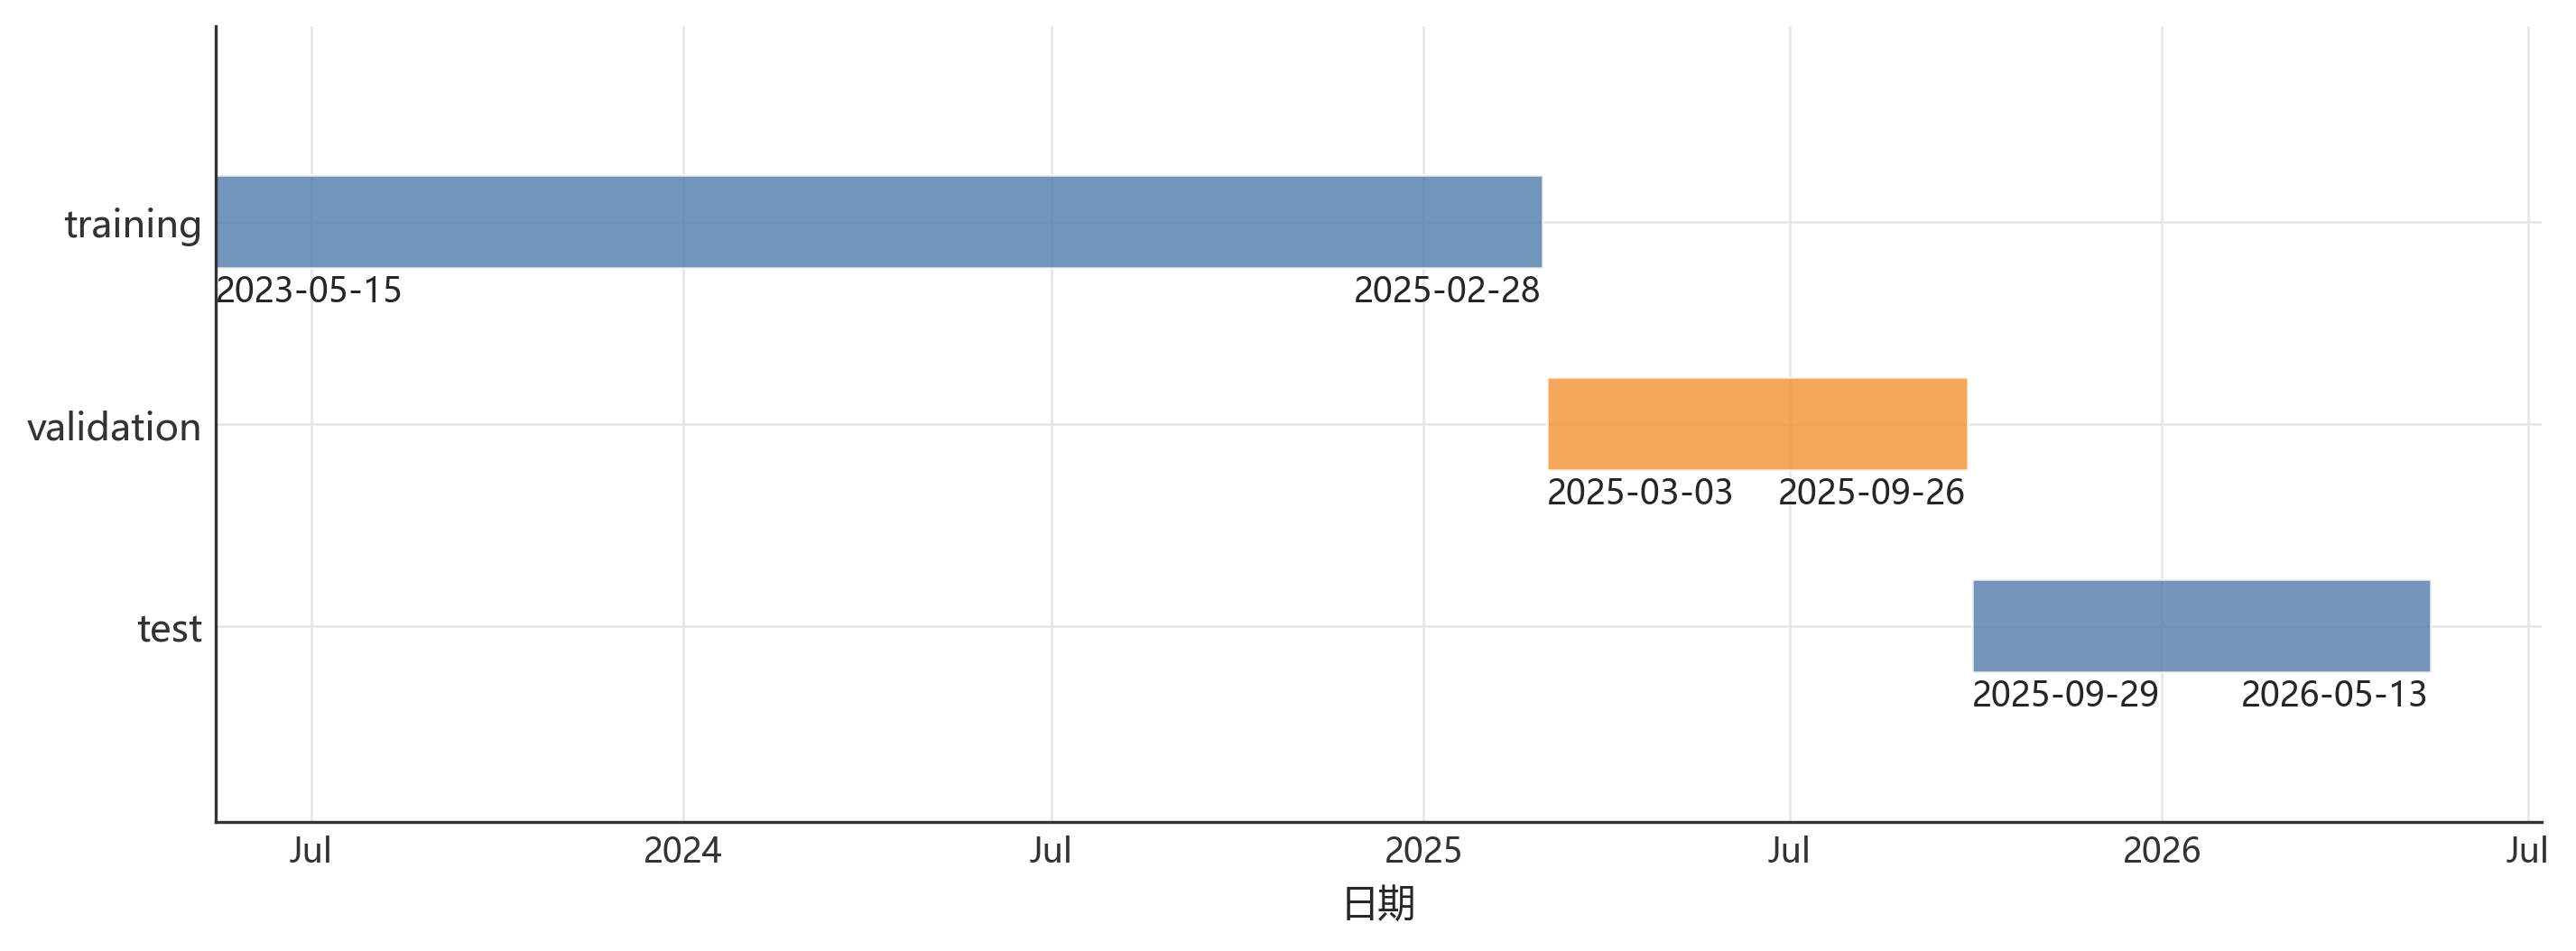
\includegraphics[width=0.72\textwidth]{figures/fig_timeline.png}
    \captionof{figure}{训练、验证与测试样本划分}
    \label{fig:timeline}
\endgroup
\end{center}

图 \ref{fig:timeline} 明确显示训练、验证与测试区间按时间顺序展开，标准化参数、标签阈值和模型选择均在测试期之前完成。


\subsection{核心变量定义}

表 \ref{tab:variables} 汇总了后续章节使用的主要变量。CrossStress 由未来压力标签横截面聚合得到，用于 QVAR 的截面状态描述；SMARTBoost 预测特征矩阵保留当前及历史可观测状态变量。

\begin{center}
\begingroup
\captionsetup{type=table}
\begin{minipage}{\textwidth}
\centering
\captionof{table}{核心变量、压力标签与时间边界}
\label{tab:variables}
\small
\begin{threeparttable}
\begin{tabularx}{\textwidth}{p{0.18\textwidth}p{0.22\textwidth}Y}
\toprule
变量 & 含义 & 构造与解释边界 \\
\midrule
LSI\(^{(k)}\) & 个股短时压力指数 & 由 ILLIQ、Range、RV 与 RelAmt 经训练期股票—日内时间片稳健标准化后合成；属于压力代理指标。 \\
MarketLSI & 市场压力指数 & 个股 LSI 的横截面简单平均；仅使用当前及历史分钟信息。 \\
Stress\_H5 & 未来 5 分钟压力标签 & 未来窗口内 LSI 峰值是否超过训练期阈值；仅作为预测目标变量。 \\
Stress\_H10 & 未来 10 分钟压力标签 & 未来窗口内 LSI 峰值是否超过训练期阈值；仅作为预测目标变量。 \\
IndexRet & 市场收益状态 & 分钟收益率的横截面平均，用于 QVAR 和预警特征。 \\
IndexRV & 市场波动状态 & 分钟收益率平方的横截面平均，用于 QVAR 和预警特征。 \\
MarketRelAmt & 市场成交承接力 & 成交额相对历史基准的横截面平均；数值越低表示成交承接越弱。 \\
\bottomrule
\end{tabularx}
\begin{tablenotes}[flushleft]
\footnotesize
\item 注：CrossStress 在 QVAR 中作为截面压力状态变量，SMARTBoost 特征矩阵保留当前及历史可观测状态变量。
\end{tablenotes}
\end{threeparttable}
\end{minipage}
\endgroup
\end{center}

表 \ref{tab:variables} 将预测目标变量、当前市场状态变量和横截面压力状态变量加以区分，为后续 QVAR 描述和 SMARTBoost 样本外预警提供变量边界。


\Needspace{8\baselineskip}
\subsection{样本覆盖与数据质量}

在进入模型估计前，需确认分钟面板在证券和时间维度上具有足够稳定的覆盖。图 \ref{fig:coverage} 按股票和月份汇总有效分钟覆盖率，以热力图形式检查样本是否存在系统性缺口。

\begin{center}
\begingroup
\captionsetup{type=figure}
    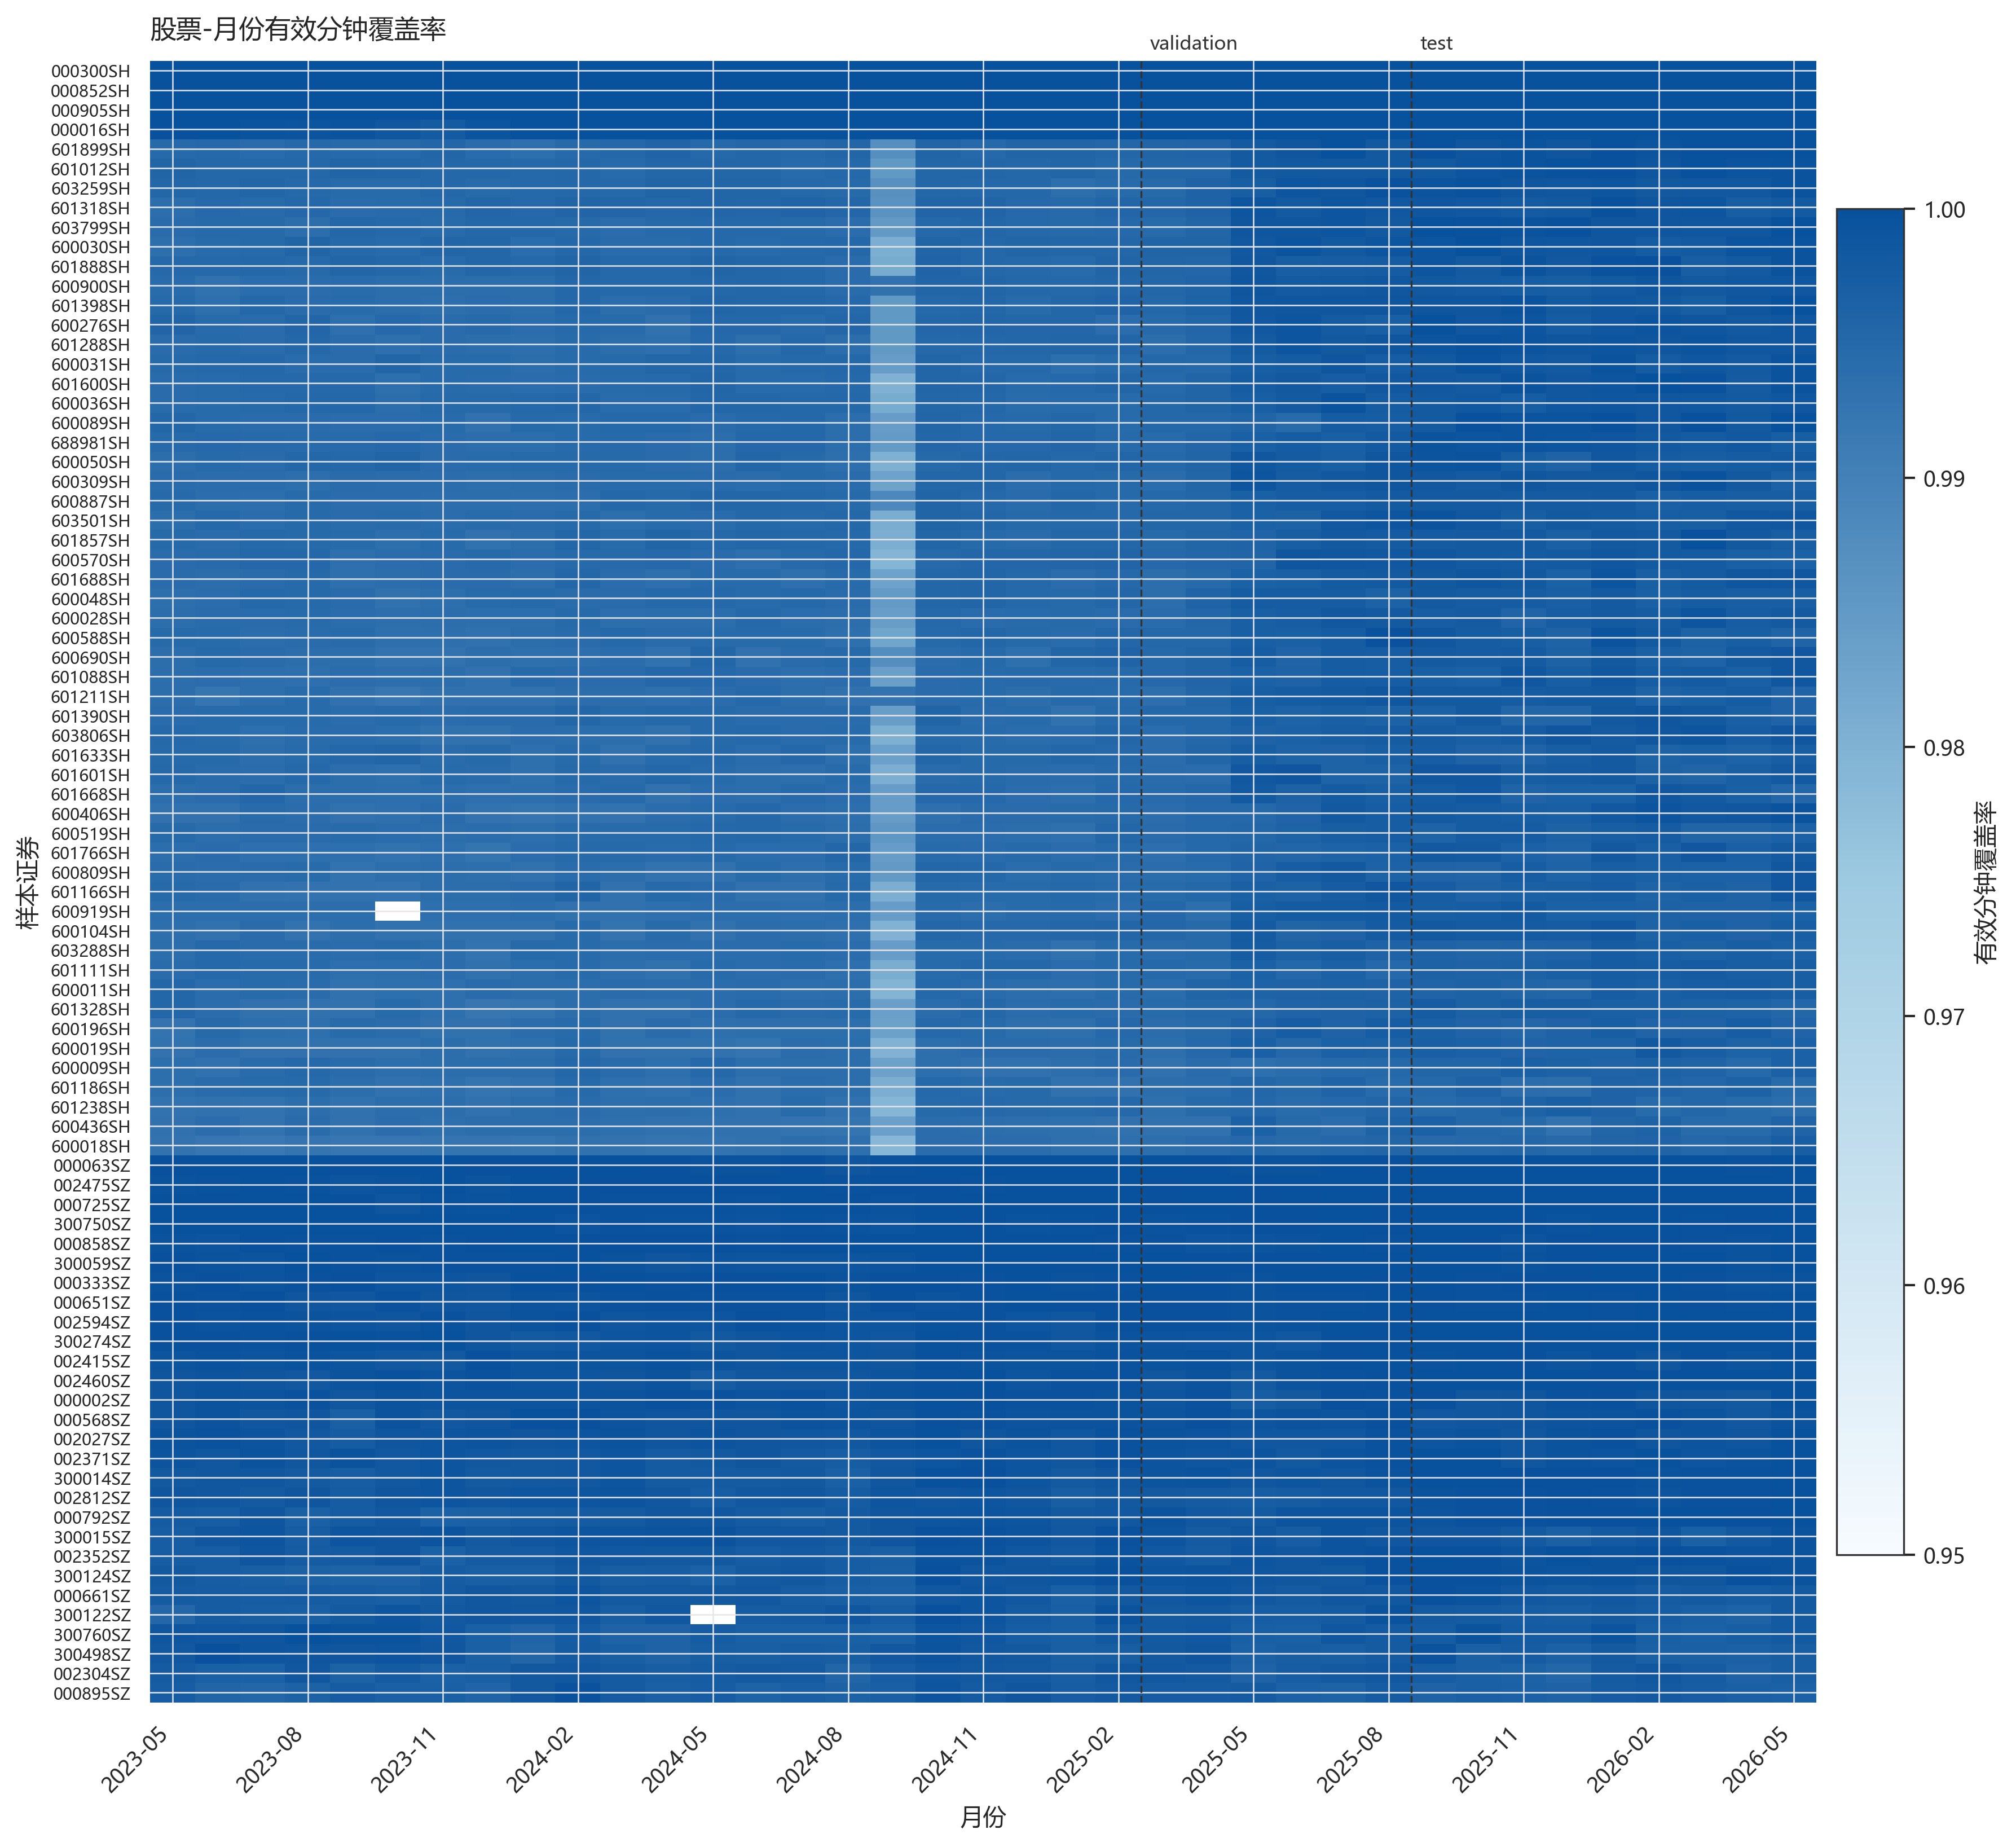
\includegraphics[width=0.78\textwidth]{figures/fig_coverage.png}
    \captionof{figure}{股票—月份有效分钟覆盖率热力图}
    \label{fig:coverage}
\endgroup
\end{center}

图 \ref{fig:coverage} 表明，样本在多数股票和月份上具有较稳定的有效分钟覆盖，未呈现集中于单一时期或单一证券的系统性缺口，后续分析可以建立在相对完整的高频面板之上。图中个别浅色区域对应特定证券在局部月份的有效分钟覆盖下降，主要源于阶段性停牌或数据报送差异，属于局部现象，不构成跨时期的系统性样本偏误。训练、验证与测试三个区间的整体覆盖水平较为接近，有助于排除样本外检验结论由测试期数据缺失所导致的可能性。

\Needspace{8\baselineskip}
\subsection{LSI 日内模式}

高频压力指标具有明显的日内结构特征。图 \ref{fig:intraday} 展示了 $\LSI_{5}$ 在不同日内时间片上的均值、中位数和分位带。

\begin{center}
\begingroup
\captionsetup{type=figure}
    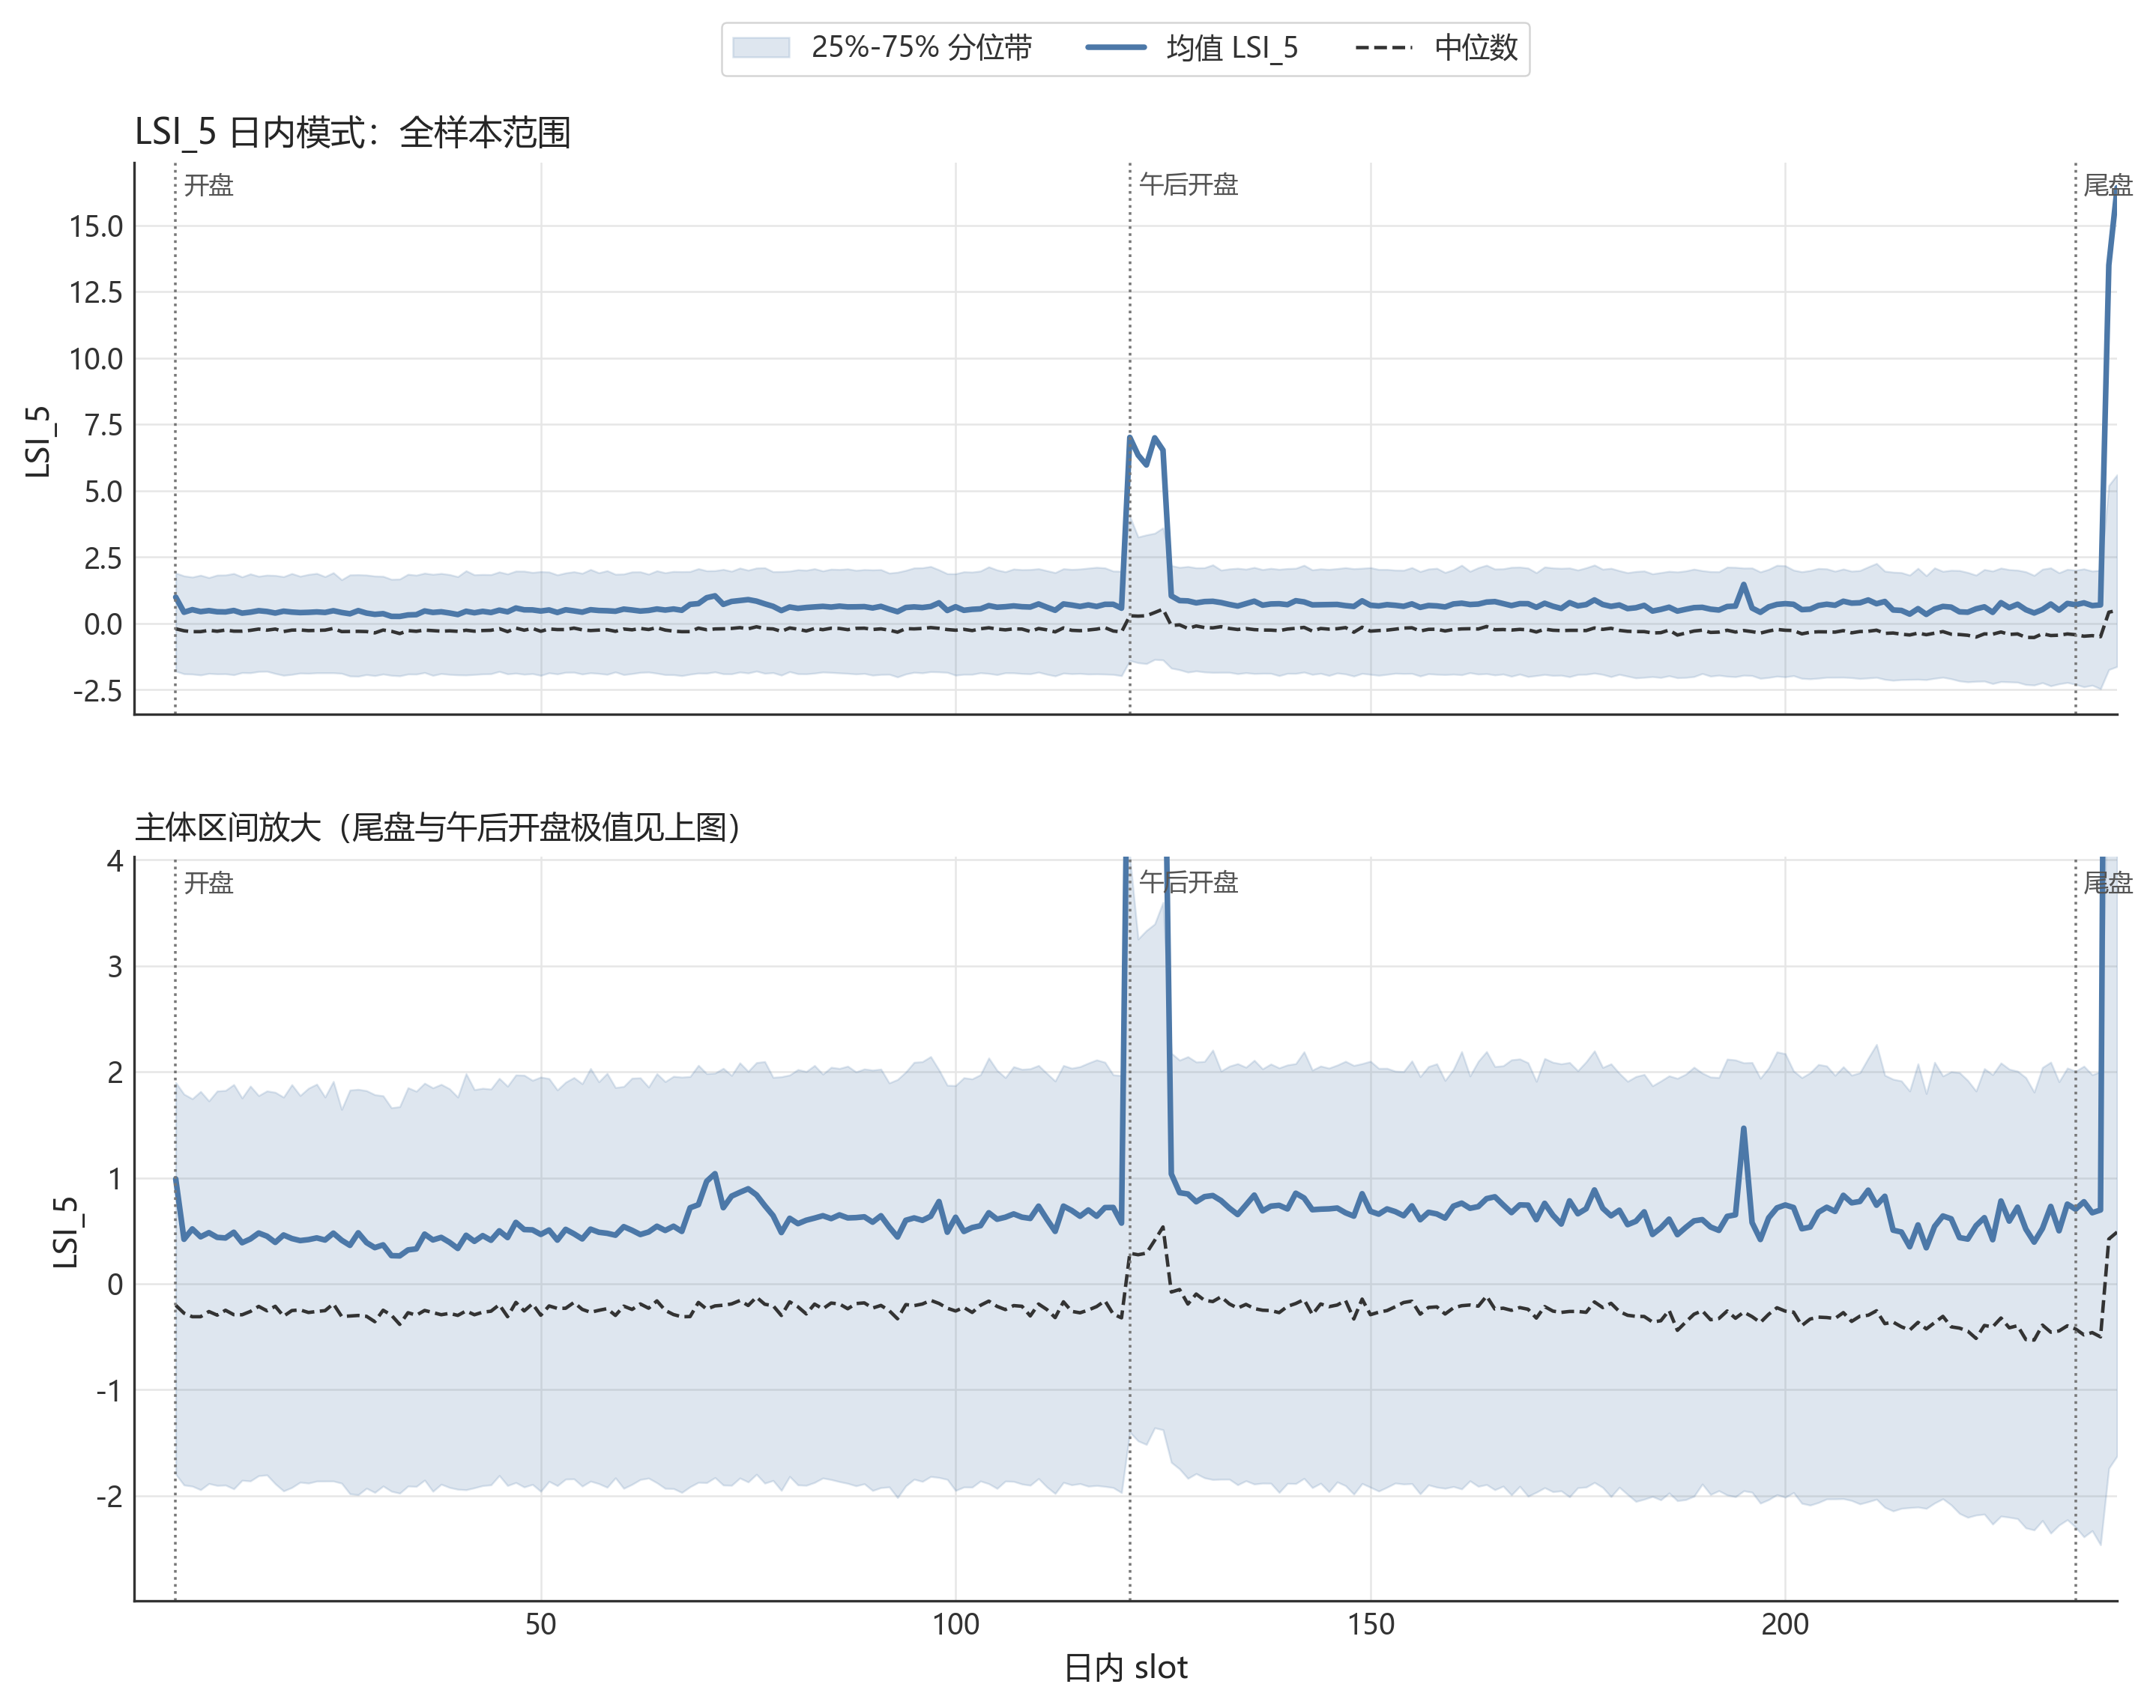
\includegraphics[width=0.86\textwidth,height=0.50\textheight,keepaspectratio]{figures/fig_intraday.png}
    \captionof{figure}{LSI\_5 日内模式}
    \label{fig:intraday}
\endgroup
\end{center}

LSI 在开盘、午后开盘和尾盘附近更容易出现局部抬升，说明短时压力具有与交易节奏相关的系统性日内结构。高频流动性压力的日内节奏意味着，若不加以控制地跨时间片比较样本，可能将开盘或尾盘附近的正常交易节律误判为异常压力抬升。本文在股票—日内时间片层面使用训练期历史分布确定标准化参数，目的是使后续特征和标签尽量反映相对于正常节律的偏离程度，而不是吸收时间片本身的固定效应。

\subsection{MarketLSI 与压力事件率}

图 \ref{fig:marketlsi} 将 MarketLSI 按日聚合，并叠加滚动趋势线与样本区间背景。

\begin{center}
\begingroup
\captionsetup{type=figure}
    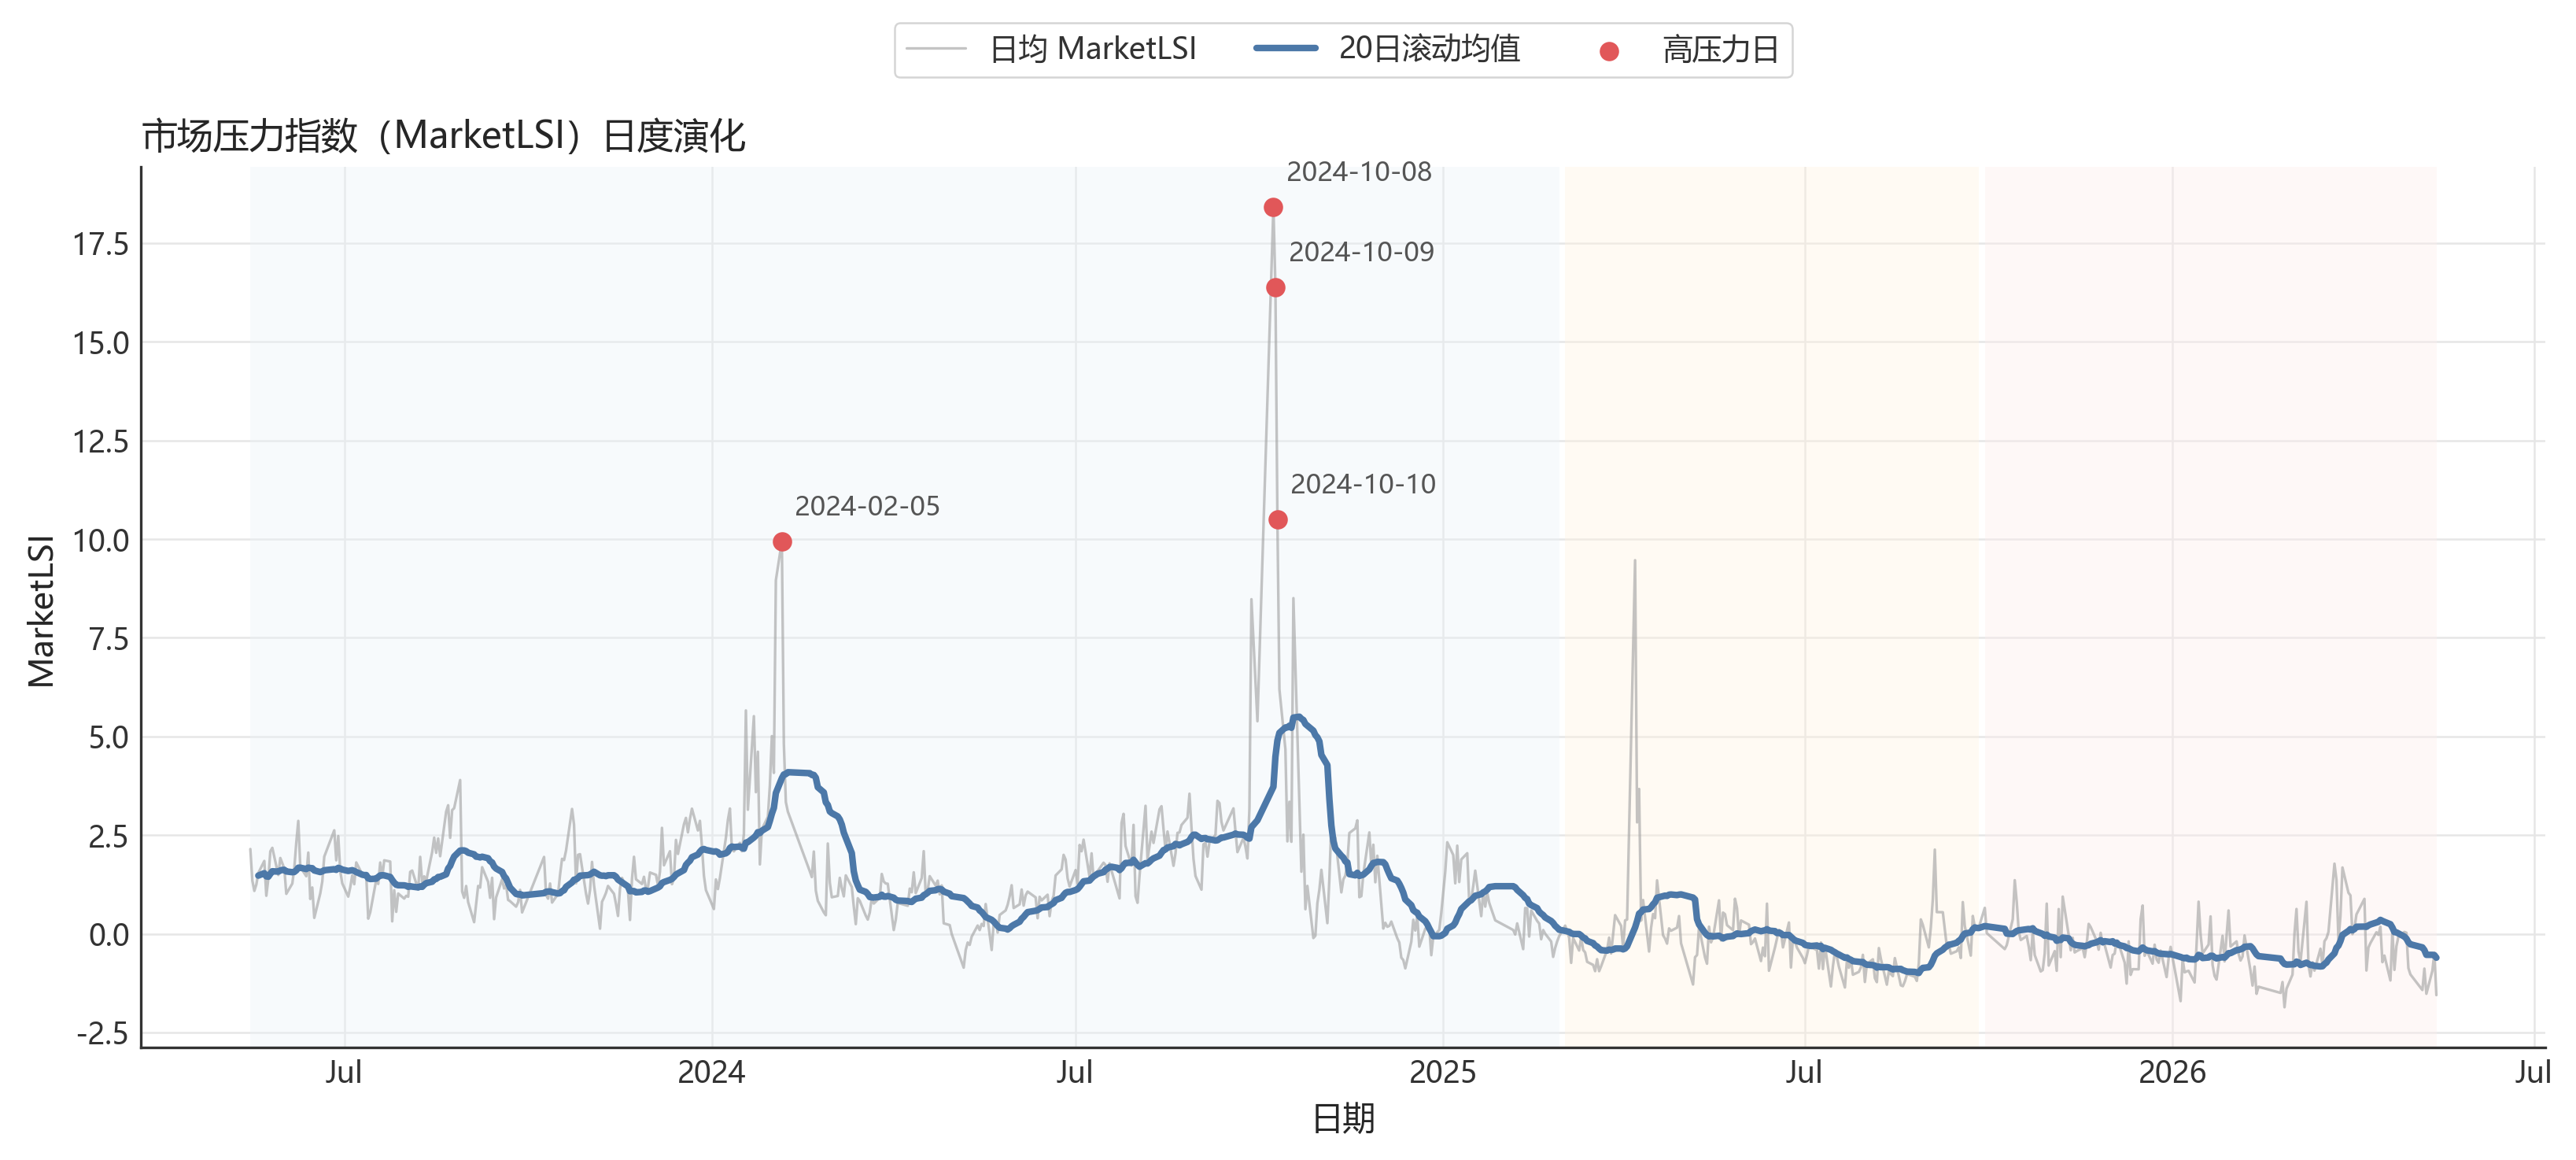
\includegraphics[width=0.82\textwidth]{figures/fig_marketlsi.png}
    \captionof{figure}{MarketLSI 日度时间序列}
    \label{fig:marketlsi}
\endgroup
\end{center}

MarketLSI 在样本期内呈现出明显的阶段性抬升和局部峰值，高压力阶段往往与特定市场事件时段相吻合。上述三个峰值时段的形成机制各有不同，但均具有明确的市场事件对应性。2024 年 2 月初，A 股在经历小微盘持续下跌和市场信心快速收缩后，于 2 月 5 日盘中出现大范围个股下跌与跌停现象，监管层随后就异常波动和恶意做空问题作出稳定市场表态。图中 2024 年 2 月附近的 MarketLSI 峰值，反映出极端下跌阶段下成交承接能力下降、价格振幅扩大与短时波动上升的共同作用，是典型的流动性踩踏驱动型压力事件。2024 年 10 月，市场在政策预期推动下先经历极端放量上涨，国庆节后随即转入高位分歧与大幅回调；10 月 8 日至 10 日附近的连续峰值，对应的是交易拥挤、获利了结与预期再定价交织下的短时市场压力，其峰值绝对水平为样本期最高，反映出极度乐观情绪骤然逆转时的流动性耗竭特征。2025 年 4 月 7 日前后，中美关税冲突升级引发全球风险资产同步调整，A 股三大指数大幅低开下行，图中亦可观察到 MarketLSI 的局部抬升；相较于前两次峰值，此次抬升幅度相对温和，在一定程度上反映了彼时市场整体仓位水平偏低以及稳市机制的快速介入。
综合来看，MarketLSI 的峰值并非孤立的统计异常，而是在重大市场冲击、交易拥挤和流动性承接弱化阶段具有较强的事件对应性。三次峰值在驱动因素上覆盖了杠杆产品集中平仓、情绪过热后的预期落差以及外部宏观冲击三类典型情景，表明 MarketLSI 能够跨越不同冲击类型，较为稳健地捕捉分钟级市场状态中蕴含的短时流动性压力信息。

表 \ref{tab:label-distribution} 给出未来压力标签在各样本区间的事件率分布。训练期事件率接近 10\%，而验证期和测试期降至约 5\%--6\%，反映出样本外预警任务的高度不平衡性。这也是本文在 SMARTBoost 评价中优先使用 PR-AUC、Top 5\% 命中率和提升倍数的原因。

\begin{center}
\begingroup
\captionsetup{type=table}
\begin{minipage}{\textwidth}
\centering
\captionof{table}{未来压力标签的样本区间分布}
\label{tab:label-distribution}
\small
\begin{threeparttable}
\begin{tabular}{lcc}
\toprule
样本区间 & Stress\_H5 事件率 & Stress\_H10 事件率 \\
\midrule
train & 10.05\% & 10.06\% \\
验证集 & 5.05\% & 5.27\% \\
测试集 & 5.44\% & 5.80\% \\
\bottomrule
\end{tabular}
\begin{tablenotes}[flushleft]
\footnotesize
\item 注：标签阈值由训练期历史分布唯一确定。
\end{tablenotes}
\end{threeparttable}
\end{minipage}
\endgroup
\end{center}

表 \ref{tab:label-distribution} 进一步说明，样本外阶段事件率较训练期更低，预警模型需要在较低基准率下保持高风险排序能力。


% ============================================================
% 5 实证结果分析
% ============================================================
\section{实证结果分析}

本章按照三层递进证据链的逻辑依次报告实证结果。第 5.1 节通过 RGARCH-CARR-SK 描述 MarketLSI 压力风险的动态聚集特征及其对已实现压力测度的敏感性；第 5.2 节通过 QVAR 考察市场状态变量在尾部分位下的条件联动与情景响应；第 5.3 节通过 SMARTBoost 直接检验历史高频特征对未来压力事件的样本外预警能力。第 5.4 节对三类证据进行综合解释。

\subsection{RGARCH-CARR-SK 动态压力风险结果}
\label{subsec:rgarch-results}

条件压力风险路径用于检验 MarketLSI 中是否存在持续的高压力状态。若 $\lambda_t$ 在 MarketLSI 局部高值附近同步上行，说明该代理指标包含可递推的风险状态信息。图 \ref{fig:rgarch-risk} 报告 RGARCH-CARR-SK 估计得到的条件压力风险 $\lambda_t$ 路径。

\begin{center}
\begingroup
\captionsetup{type=figure}
    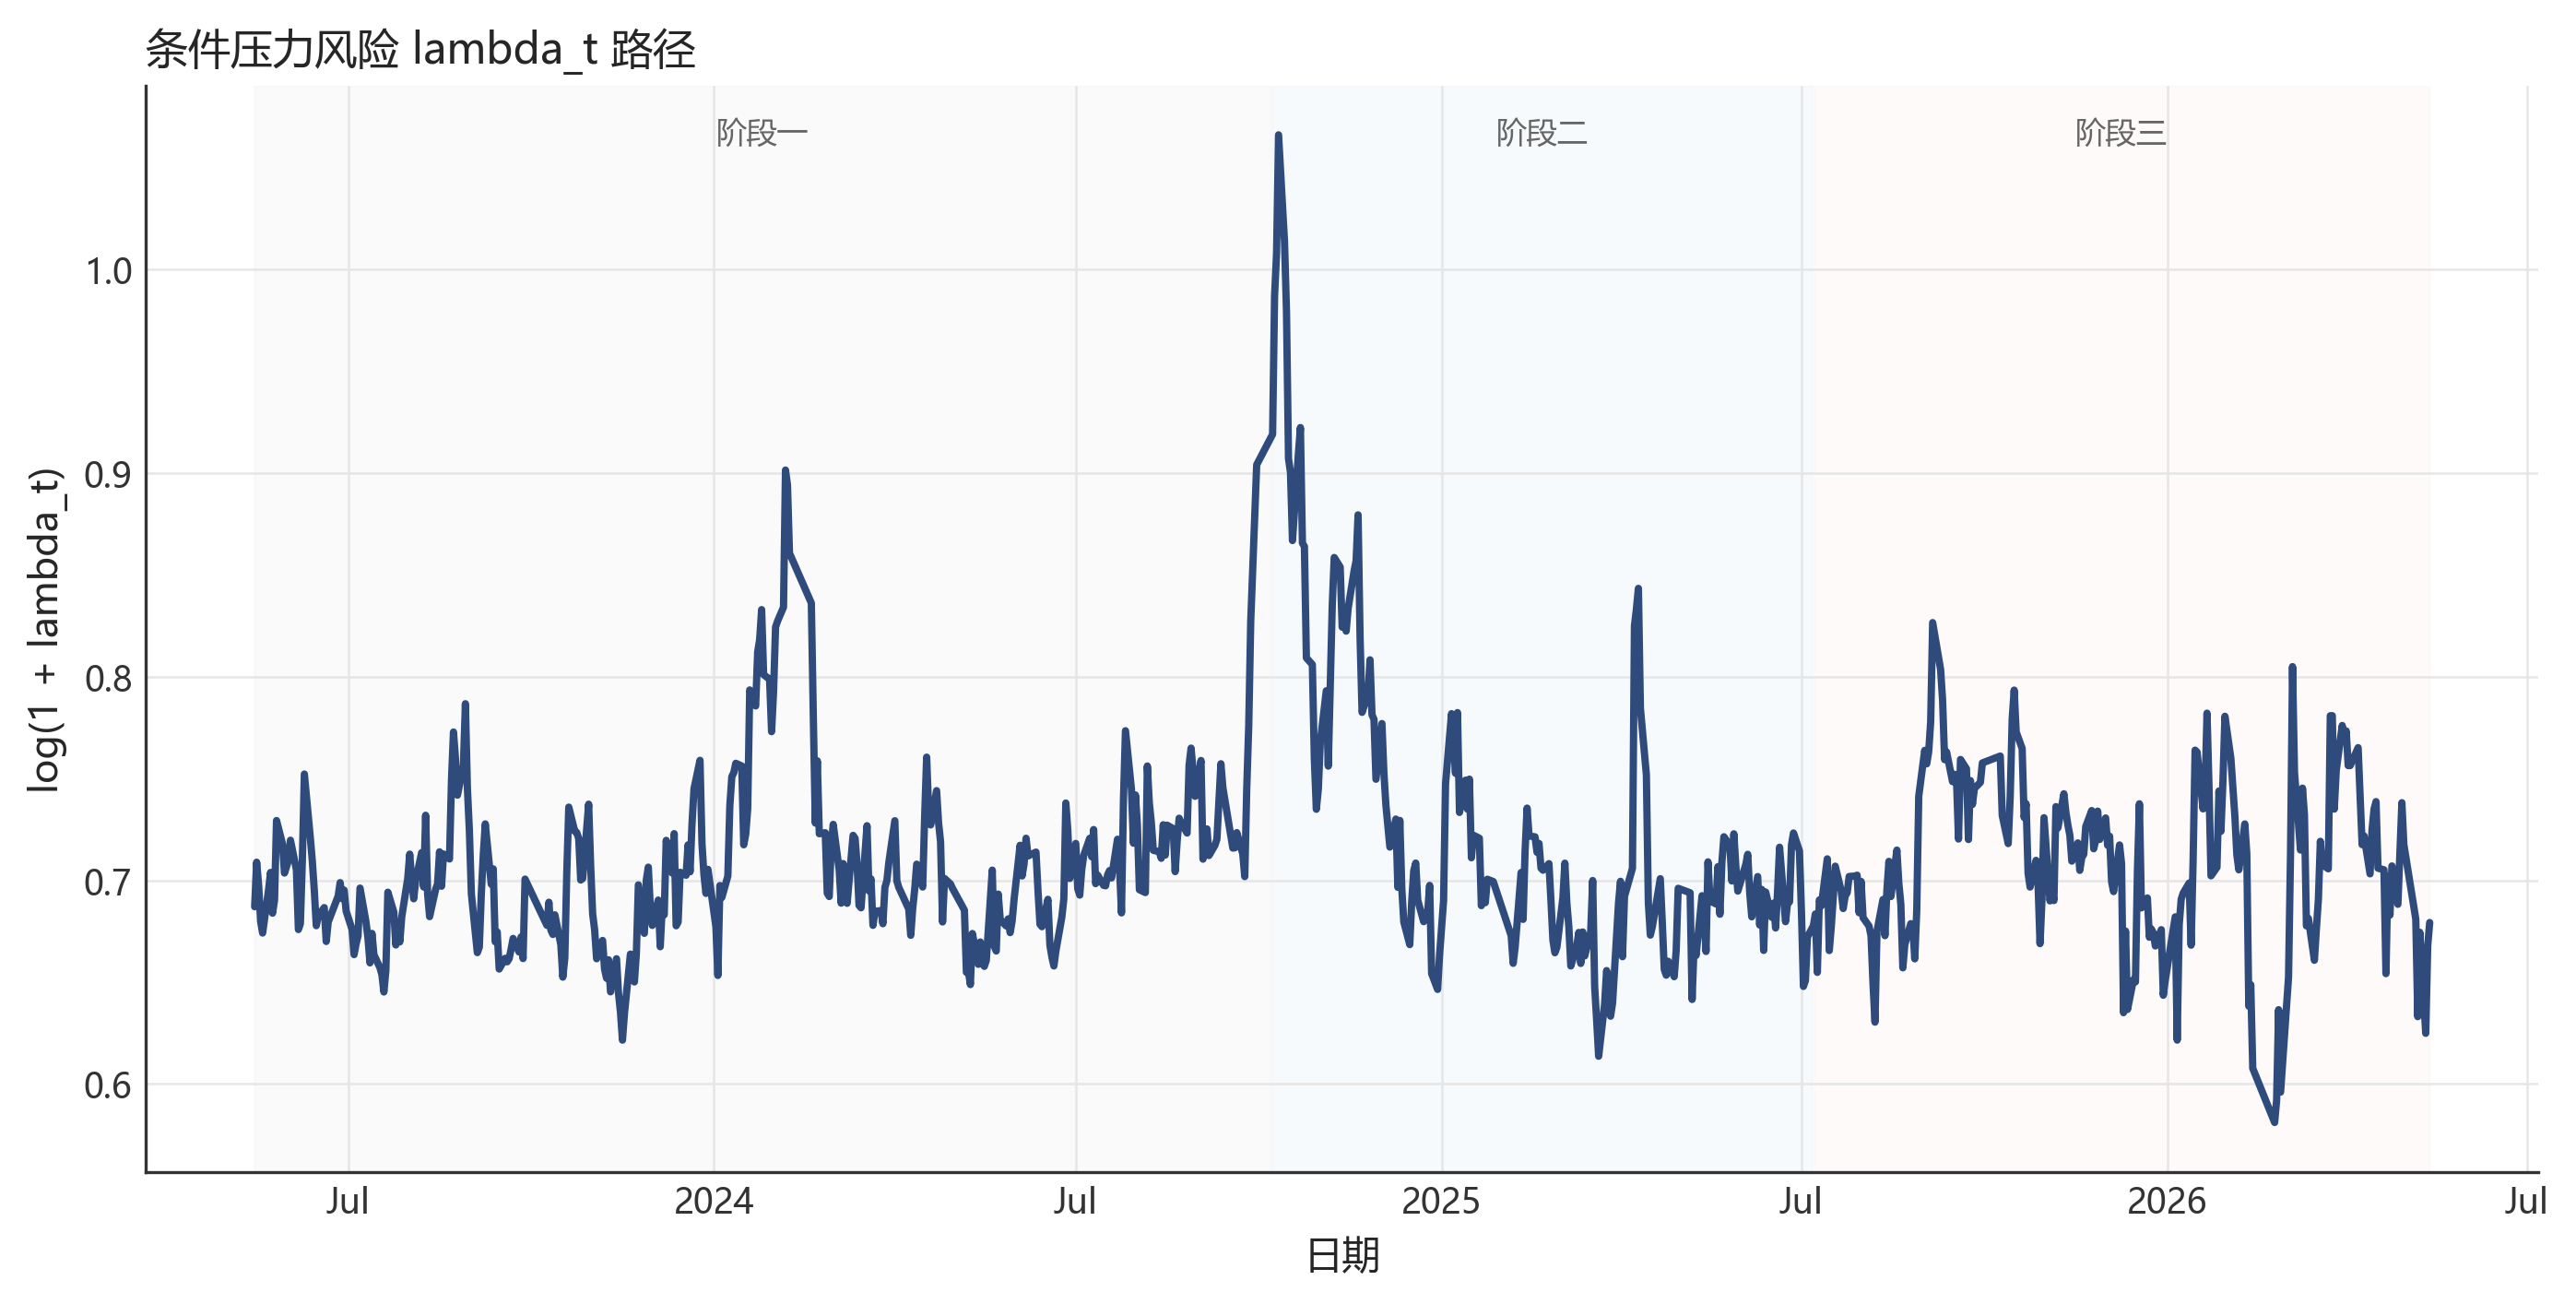
\includegraphics[width=0.78\linewidth,height=0.31\textheight,keepaspectratio]{figures/fig_rgarch_risk.png}
    \captionof{figure}{RGARCH-CARR-SK 条件压力风险路径}
    \label{fig:rgarch-risk}
\endgroup
\end{center}

图 \ref{fig:rgarch-risk} 显示，条件压力风险 $\lambda_t$ 在若干阶段出现明显抬升，且与 MarketLSI 局部峰值时段大体对应。这表明已实现压力测度能够为风险递推提供有效信息，MarketLSI 具有一定的时间聚集特征。

从 $\lambda_t$ 的经济意义看，条件压力风险水平的持续抬升表明 MarketLSI 的压力状态具有跨分钟的时间聚集性，而不表现为逐分钟独立的随机波动。递推结构将已实现压力测度的历史信息延续至当前风险估计，使得高压力阶段的 $\lambda_t$ 不会因单个低压力分钟而骤然消散。

RGARCH-CARR-SK 框架还允许通过动态高阶矩刻画压力冲击分布的形状变化。动态高阶矩主要作为压力冲击分布非对称性的诊断信息，图 \ref{fig:rgarch_dynamic_skewness} 报告动态偏度 $s_t$ 的时间路径。

\begin{center}
\begingroup
\captionsetup{type=figure}
    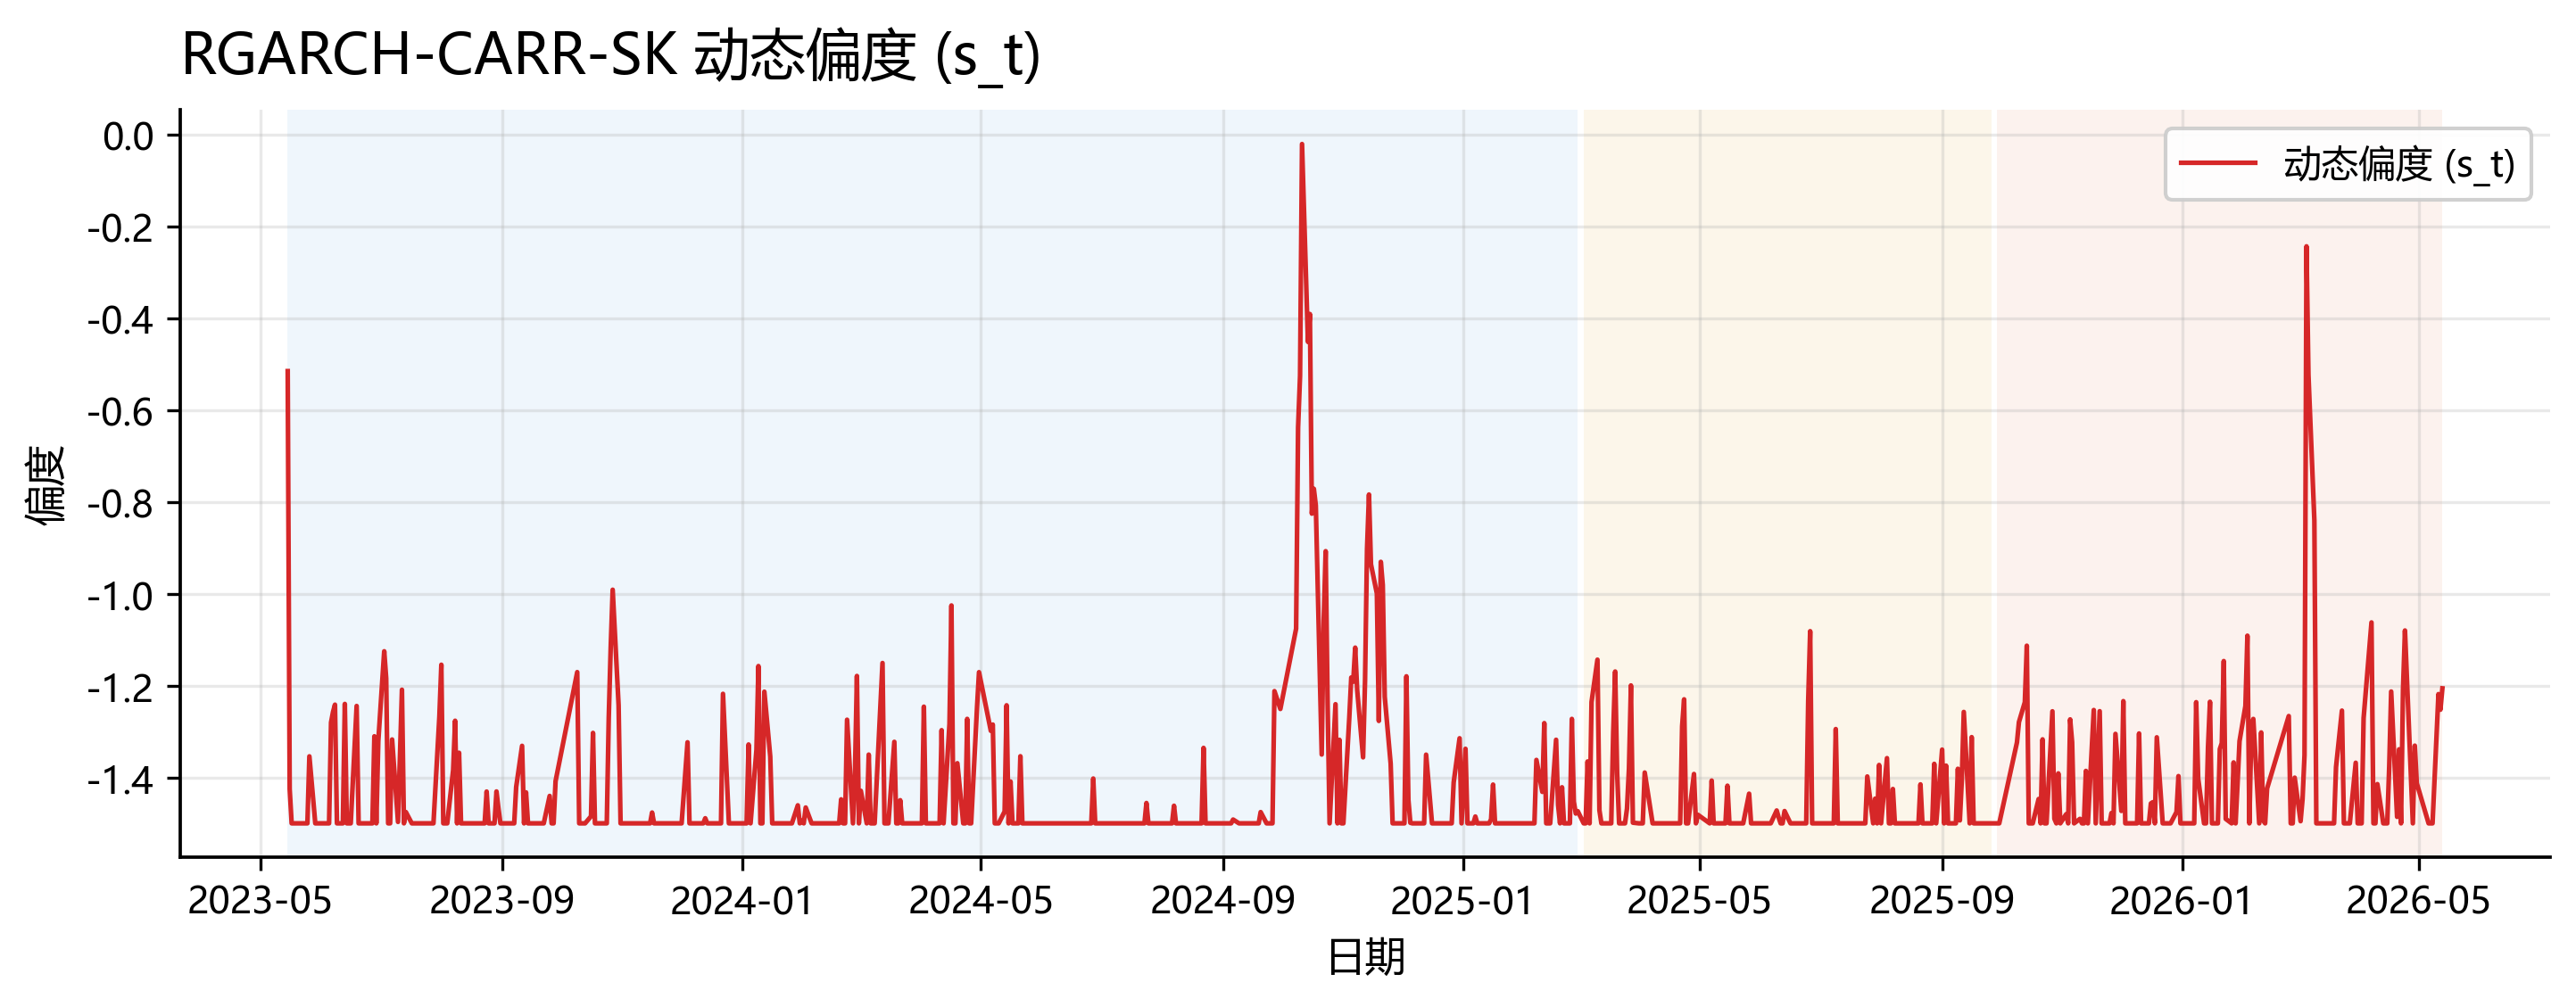
\includegraphics[width=0.78\linewidth,height=0.31\textheight,keepaspectratio]{figures/fig_rgarch_dynamic_skewness_refined.png}
    \captionof{figure}{RGARCH-CARR-SK 动态偏度 $s_t$ 路径}
    \label{fig:rgarch_dynamic_skewness}
\endgroup
\end{center}

动态偏度 $s_t$ 在大部分时期位于负值区间，并在若干局部压力阶段出现向零附近的快速抬升，表明 MarketLSI 压力冲击不仅体现为条件风险水平的上升，也伴随着冲击分布非对称性的阶段性变化。

为进一步检验上述风险路径是否依赖已实现压力测度的具体口径，表 \ref{tab:rgarch-fit} 先比较四类测度下的样本内拟合准则。

\begin{center}
\begingroup
\captionsetup{type=table}
\begin{minipage}{\textwidth}
\centering
\captionof{table}{RGARCH-CARR-SK 拟合准则}
\label{tab:rgarch-fit}
\small
\begin{threeparttable}
\begin{tabular}{lrrr}
\toprule
已实现测度 & LLK & AIC & BIC \\
\midrule
RV & -169.822 & 365.64 & 418.62 \\
RBV & -198.783 & 423.57 & 476.54 \\
MedRV & -203.959 & 433.92 & 486.90 \\
RMAD & -553.492 & 1,133 & 1,186 \\
\bottomrule
\end{tabular}
\begin{tablenotes}[flushleft]
\footnotesize
\item 注：LLK、AIC 和 BIC 用于比较不同已实现压力测度下的样本内拟合表现。
\end{tablenotes}
\end{threeparttable}
\end{minipage}
\endgroup
\end{center}

表 \ref{tab:rgarch-fit} 显示，不同已实现压力测度对样本内拟合准则有明显影响。接下来，表 \ref{tab:rgarch-loss} 从样本外损失角度检验这种口径差异是否延续到验证集和测试集。

\begin{center}
\begingroup
\captionsetup{type=table}
\begin{minipage}{\textwidth}
\centering
\captionof{table}{RGARCH-CARR-SK 样本外损失}
\label{tab:rgarch-loss}
\small
\begin{threeparttable}
\begin{tabular}{lrrr}
\toprule
已实现测度 & R2LOG（验证集） & R2LOG（测试集） & MAE（测试集） \\
\midrule
RV & 15.605 & 15.396 & 53.392 \\
RBV & 15.578 & 15.266 & 53.420 \\
MedRV & 16.855 & 16.693 & 53.378 \\
RMAD & 0.020 & 0.030 & 0.131 \\
\bottomrule
\end{tabular}
\begin{tablenotes}[flushleft]
\footnotesize
\item 注：R2LOG 为损失指标，数值越低越好。RMAD 的 R2LOG 明显低于其他测度，该差异与测度尺度及压力序列构造方式有关，需要结合尺度差异审慎解释。
\end{tablenotes}
\end{threeparttable}
\end{minipage}
\endgroup
\end{center}

不同已实现压力测度会改变模型的拟合表现和样本外损失，说明条件压力风险路径对测度口径具有敏感性。RMAD 在 R2LOG 上表现较低，但该差异主要来源于测度尺度的差异。这一结果提示，压力风险路径的解释需要结合已实现压力测度的统计属性展开。RV、RBV、MedRV 与 RMAD 在刻画分布中心和尾部信息时的统计属性各异，进而使条件压力风险估计对测度口径较为敏感；这与高频波动文献中不同已实现测度对微观结构噪声具有不同稳健性的观点一致，也提示测度敏感性本身应被视为需要报告的建模设定信息。

综上，RGARCH-CARR-SK 提供了本文的第一层证据：MarketLSI 压力风险具有可度量的阶段性聚集特征，且风险路径对已实现压力测度的选择较为敏感。这为后续 QVAR 和 SMARTBoost 分析提供了动态风险背景。


\Needspace{8\baselineskip}
\subsection{QVAR 尾部分位传导与压力测试}
\label{subsec:qvar-results}

QVAR 进一步考察 MarketLSI 与市场收益、市场波动、成交承接状态之间的多变量条件分位联动。表 \ref{tab:qvar-pinball} 首先报告 MarketLSI 方程在不同分位点下的样本外分位损失。

\begin{center}
\begingroup
\captionsetup{type=table}
\begin{minipage}{\textwidth}
\centering
\captionof{table}{QVAR MarketLSI 方程样本外分位损失}
\label{tab:qvar-pinball}
\small
\begin{tabular}{lrrr}
\toprule
样本区间 & 分位点 & MarketLSI 分位损失 & 观测数 \\
\midrule
验证集 & 0.10 & 0.0279 & 33,350 \\
验证集 & 0.50 & 0.0490 & 33,350 \\
验证集 & 0.90 & 0.0307 & 33,350 \\
验证集 & 0.95 & 0.0224 & 33,350 \\
测试集 & 0.10 & 0.0270 & 33,350 \\
测试集 & 0.50 & 0.0447 & 33,350 \\
测试集 & 0.90 & 0.0303 & 33,350 \\
测试集 & 0.95 & 0.0231 & 33,350 \\
\bottomrule
\end{tabular}
\end{minipage}
\endgroup
\end{center}

$q=0.95$ 在样本外分位损失上表现较好，表明尾部分位模型能够有效捕捉 MarketLSI 的高压力状态；而中位数与尾部分位点的差异则说明，单纯的均值关系不足以概括尾部压力状态，采用 QVAR 有助于刻画这种分位异质性。

图 \ref{fig:qvar-response} 进一步比较不同分位点下 MarketLSI 的条件响应路径，横轴为预测步长。

\begin{center}
\begingroup
\captionsetup{type=figure}
    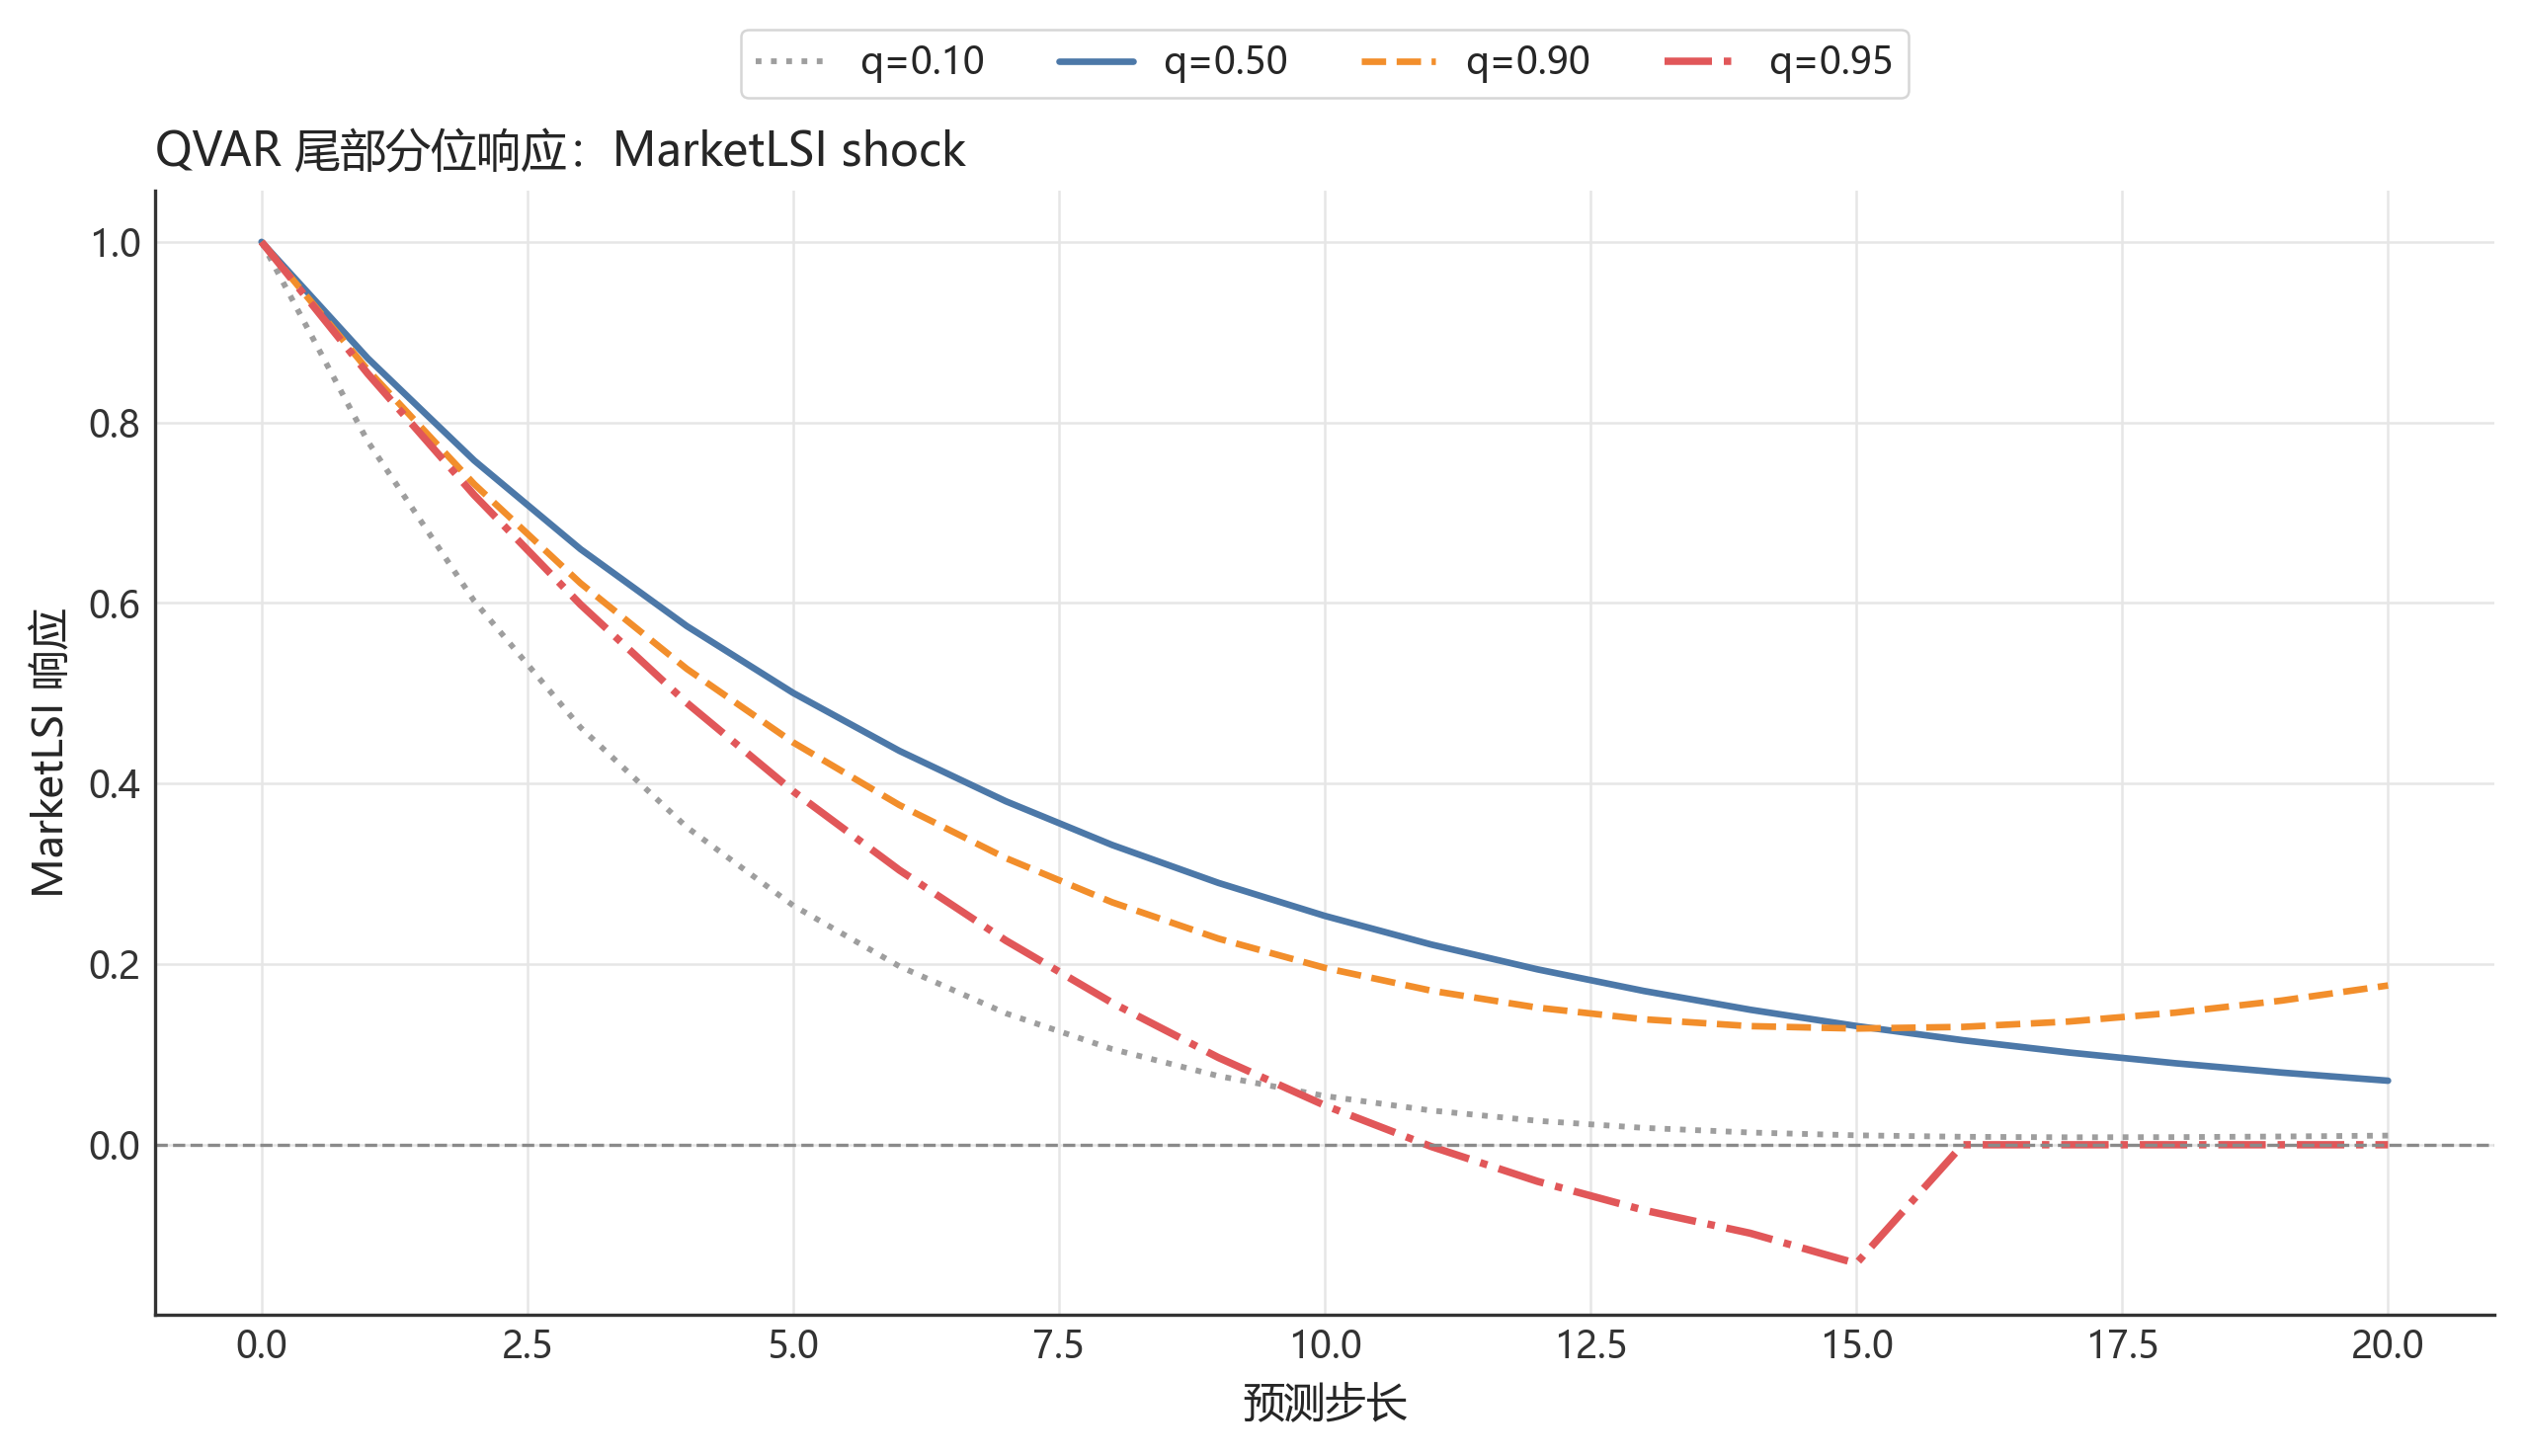
\includegraphics[width=0.78\linewidth,height=0.34\textheight,keepaspectratio]{figures/fig_qvar_response.png}
    \captionof{figure}{QVAR 尾部分位响应}
    \label{fig:qvar-response}
\endgroup
\end{center}

不同分位点下的响应路径存在明显差异。中位数状态下的响应较为平滑，而尾部分位下的路径更容易出现非对称变化，说明短时压力状态具有尾部异质性——在高分位状态下，市场状态变量的条件联动比平均水平更为显著和持久。这种尾部异质性还意味着，仅依赖中位数分位模型所提取的联动关系，会低估极端压力状态下市场变量之间的响应强度，从而使压力联动的实际程度被系统性低估。

为使尾部分位响应具有更明确的经济解释，本文构造四类标准化情景，如表 \ref{tab:qvar-scenarios} 所示。

\begin{center}
\begingroup
\captionsetup{type=table}
\begin{minipage}{\textwidth}
\centering
\captionof{table}{QVAR 压力测试情景设定}
\label{tab:qvar-scenarios}
\small
\begin{threeparttable}
\begin{tabularx}{\textwidth}{p{0.18\textwidth}p{0.34\textwidth}Y}
\toprule
情景 & 标准化冲击 & 经济含义 \\
\midrule
市场急跌 & IndexRet = -2.0 & 模拟市场收益显著下行。 \\
波动放大 & IndexRV = +2.0 & 模拟指数波动显著上升。 \\
成交收缩 & MarketRelAmt = -2.0 & 模拟成交承接能力明显下降。 \\
复合压力 & IndexRet = -2.0, IndexRV = +2.0, MarketRelAmt = -2.0 & 模拟价格、波动与成交承接同时恶化。 \\
\bottomrule
\end{tabularx}
\begin{tablenotes}[flushleft]
\footnotesize
\item 注：冲击为标准化情景模拟，用于比较不同状态设定下的相对响应。
\end{tablenotes}
\end{threeparttable}
\end{minipage}
\endgroup
\end{center}

这些情景均为标准化变量设定，用于比较不同市场状态恶化时 MarketLSI 的相对响应路径。图 \ref{fig:qvar-stress} 展示四类情景下 MarketLSI 的响应路径，用于比较不同市场状态恶化时的相对响应。

\begin{center}
\begingroup
\captionsetup{type=figure}
    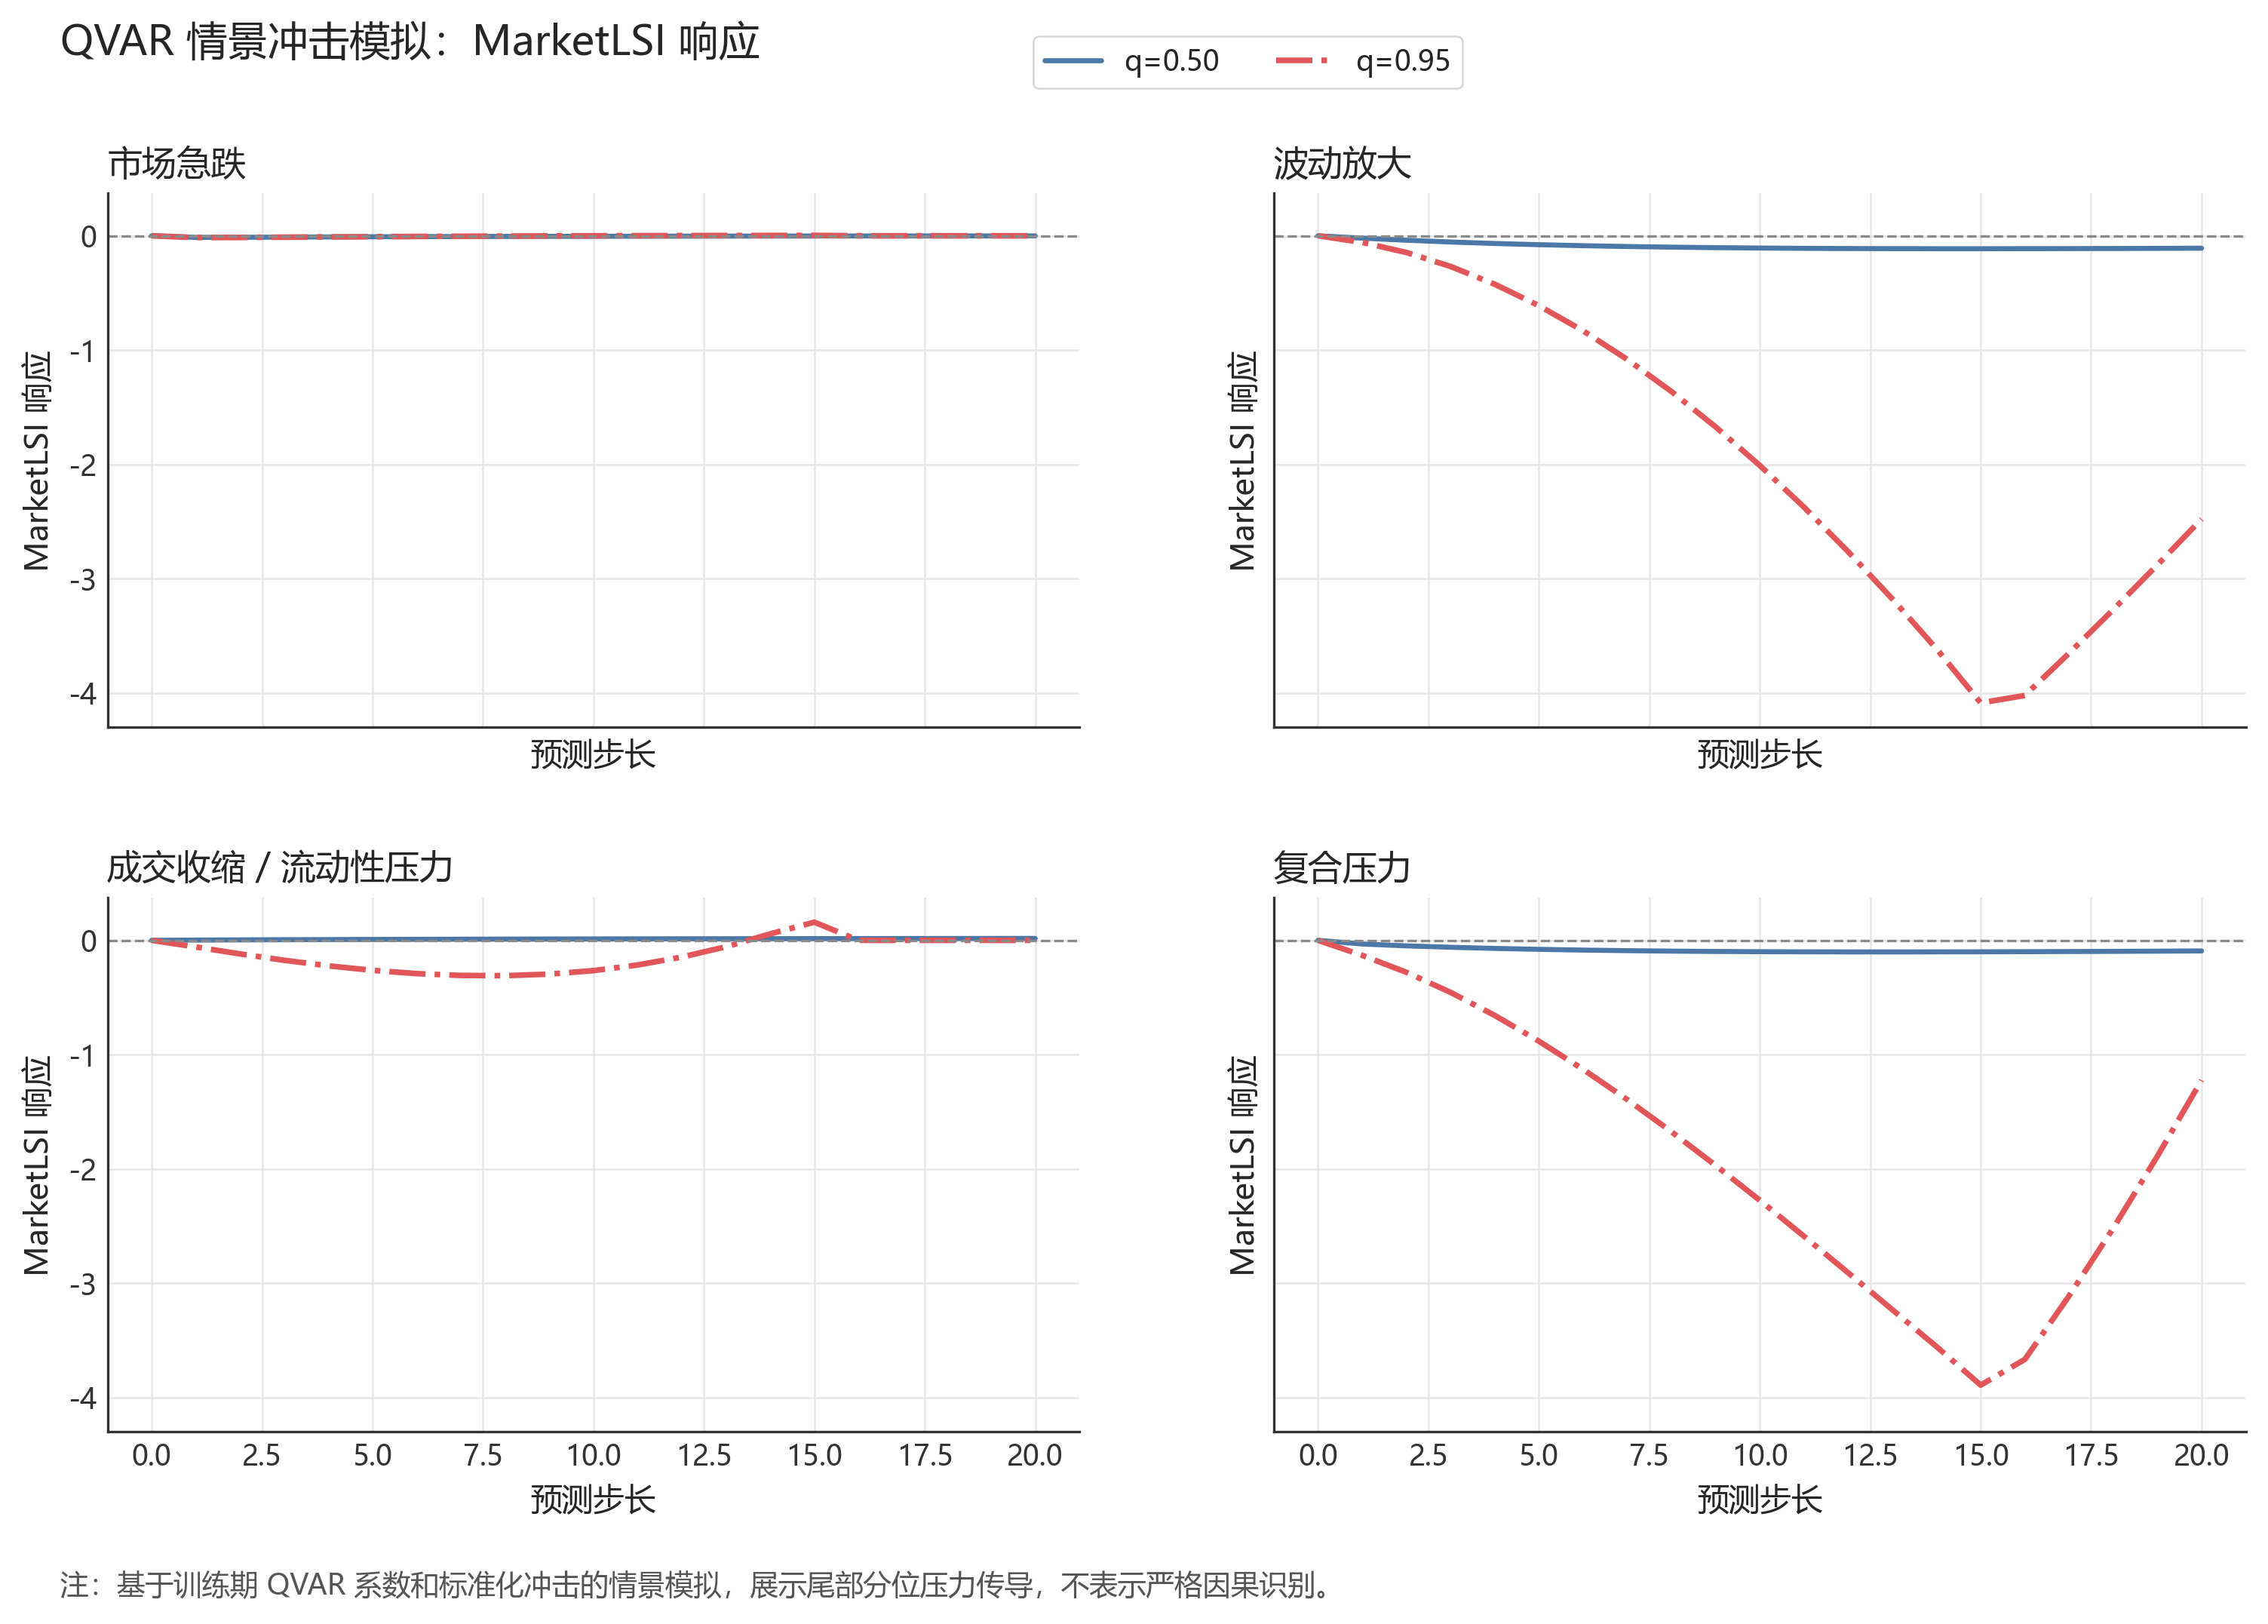
\includegraphics[width=0.82\linewidth,height=0.36\textheight,keepaspectratio]{figures/fig_qvar_stress.png}
    \captionof{figure}{QVAR 四类压力测试情景响应路径}
    \label{fig:qvar-stress}
\endgroup
\end{center}

波动放大和复合压力情景下 MarketLSI 的响应最为显著，说明短时流动性压力的形成不只来自市场收益下跌，还与波动状态和成交承接能力的变化密切相关。相比之下，单独市场急跌情景下的响应相对较弱，提示分钟级压力预警应同时纳入波动和成交承接两个维度。复合情景下响应明显强于单一情景，进一步表明多维市场状态的协同恶化会放大压力联动；这一发现为后续 SMARTBoost 将 MarketLSI、IndexRV 和 MarketRelAmt 等历史状态特征纳入预测特征提供了实证依据。

因此，QVAR 提供了本文的第二层证据：MarketLSI 与市场状态变量之间存在尾部分位联动，且压力响应在高分位状态下更为显著和非对称。


\subsection{SMARTBoost 样本外预警结果}
\label{subsec:smartboost-results}

SMARTBoost 直接检验历史分钟级状态变量能否预警未来 H5/H10 压力事件。表 \ref{tab:smartboost-metrics} 报告验证集和测试集上的主要预警指标。

\begin{center}
\begingroup
\captionsetup{type=table}
\begin{minipage}{\textwidth}
\centering
\captionof{table}{SMARTBoost 验证集/测试集样本外预警指标}
\label{tab:smartboost-metrics}
\scriptsize
\setlength{\tabcolsep}{3.8pt}
\begin{threeparttable}
\begin{tabular}{llrrrrrr}
\toprule
目标 & 区间 & 事件率 & PR-AUC & ROC-AUC & Top 5\% 命中率 & Top 5\% 召回率 & Brier \\
\midrule
H10 & 测试集 & 5.80\% & 0.545 & 0.909 & 56.42\% & 48.60\% & 0.0435 \\
H10 & 验证集 & 5.28\% & 0.528 & 0.901 & 52.02\% & 49.30\% & 0.0434 \\
H5 & 测试集 & 5.44\% & 0.603 & 0.930 & 59.30\% & 54.49\% & 0.0381 \\
H5 & 验证集 & 5.06\% & 0.589 & 0.930 & 55.63\% & 55.01\% & 0.0403 \\
\bottomrule
\end{tabular}
\begin{tablenotes}[flushleft]
\footnotesize
\item 注：Top 5\% 命中率为预测概率最高 5\% 样本中的真实压力发生率；ROC-AUC 仅作辅助参考。
\end{tablenotes}
\end{threeparttable}
\end{minipage}
\endgroup
\end{center}

测试集 H5 的 PR-AUC 为 0.603，H10 的 PR-AUC 为 0.545，均明显高于对应事件率（约 5\%--6\%）。H5 的各项指标整体高于 H10，与预期一致：更短的预测窗口内，当前压力状态与未来压力的延续性更强，历史特征的信息含量也更高。在高度不平衡的稀有事件预警任务中，PR-AUC 较 ROC-AUC 更难被多数类样本主导，因而是衡量排序能力的更敏感指标；上述结果表明模型具有超越随机排序的稀有压力事件识别能力。

由于压力事件具有明显的不平衡性，图 \ref{fig:sb-pr} 进一步展示 PR 曲线以更直接地刻画模型在高风险排序区间的表现。

\begin{center}
\begingroup
\captionsetup{type=figure}
    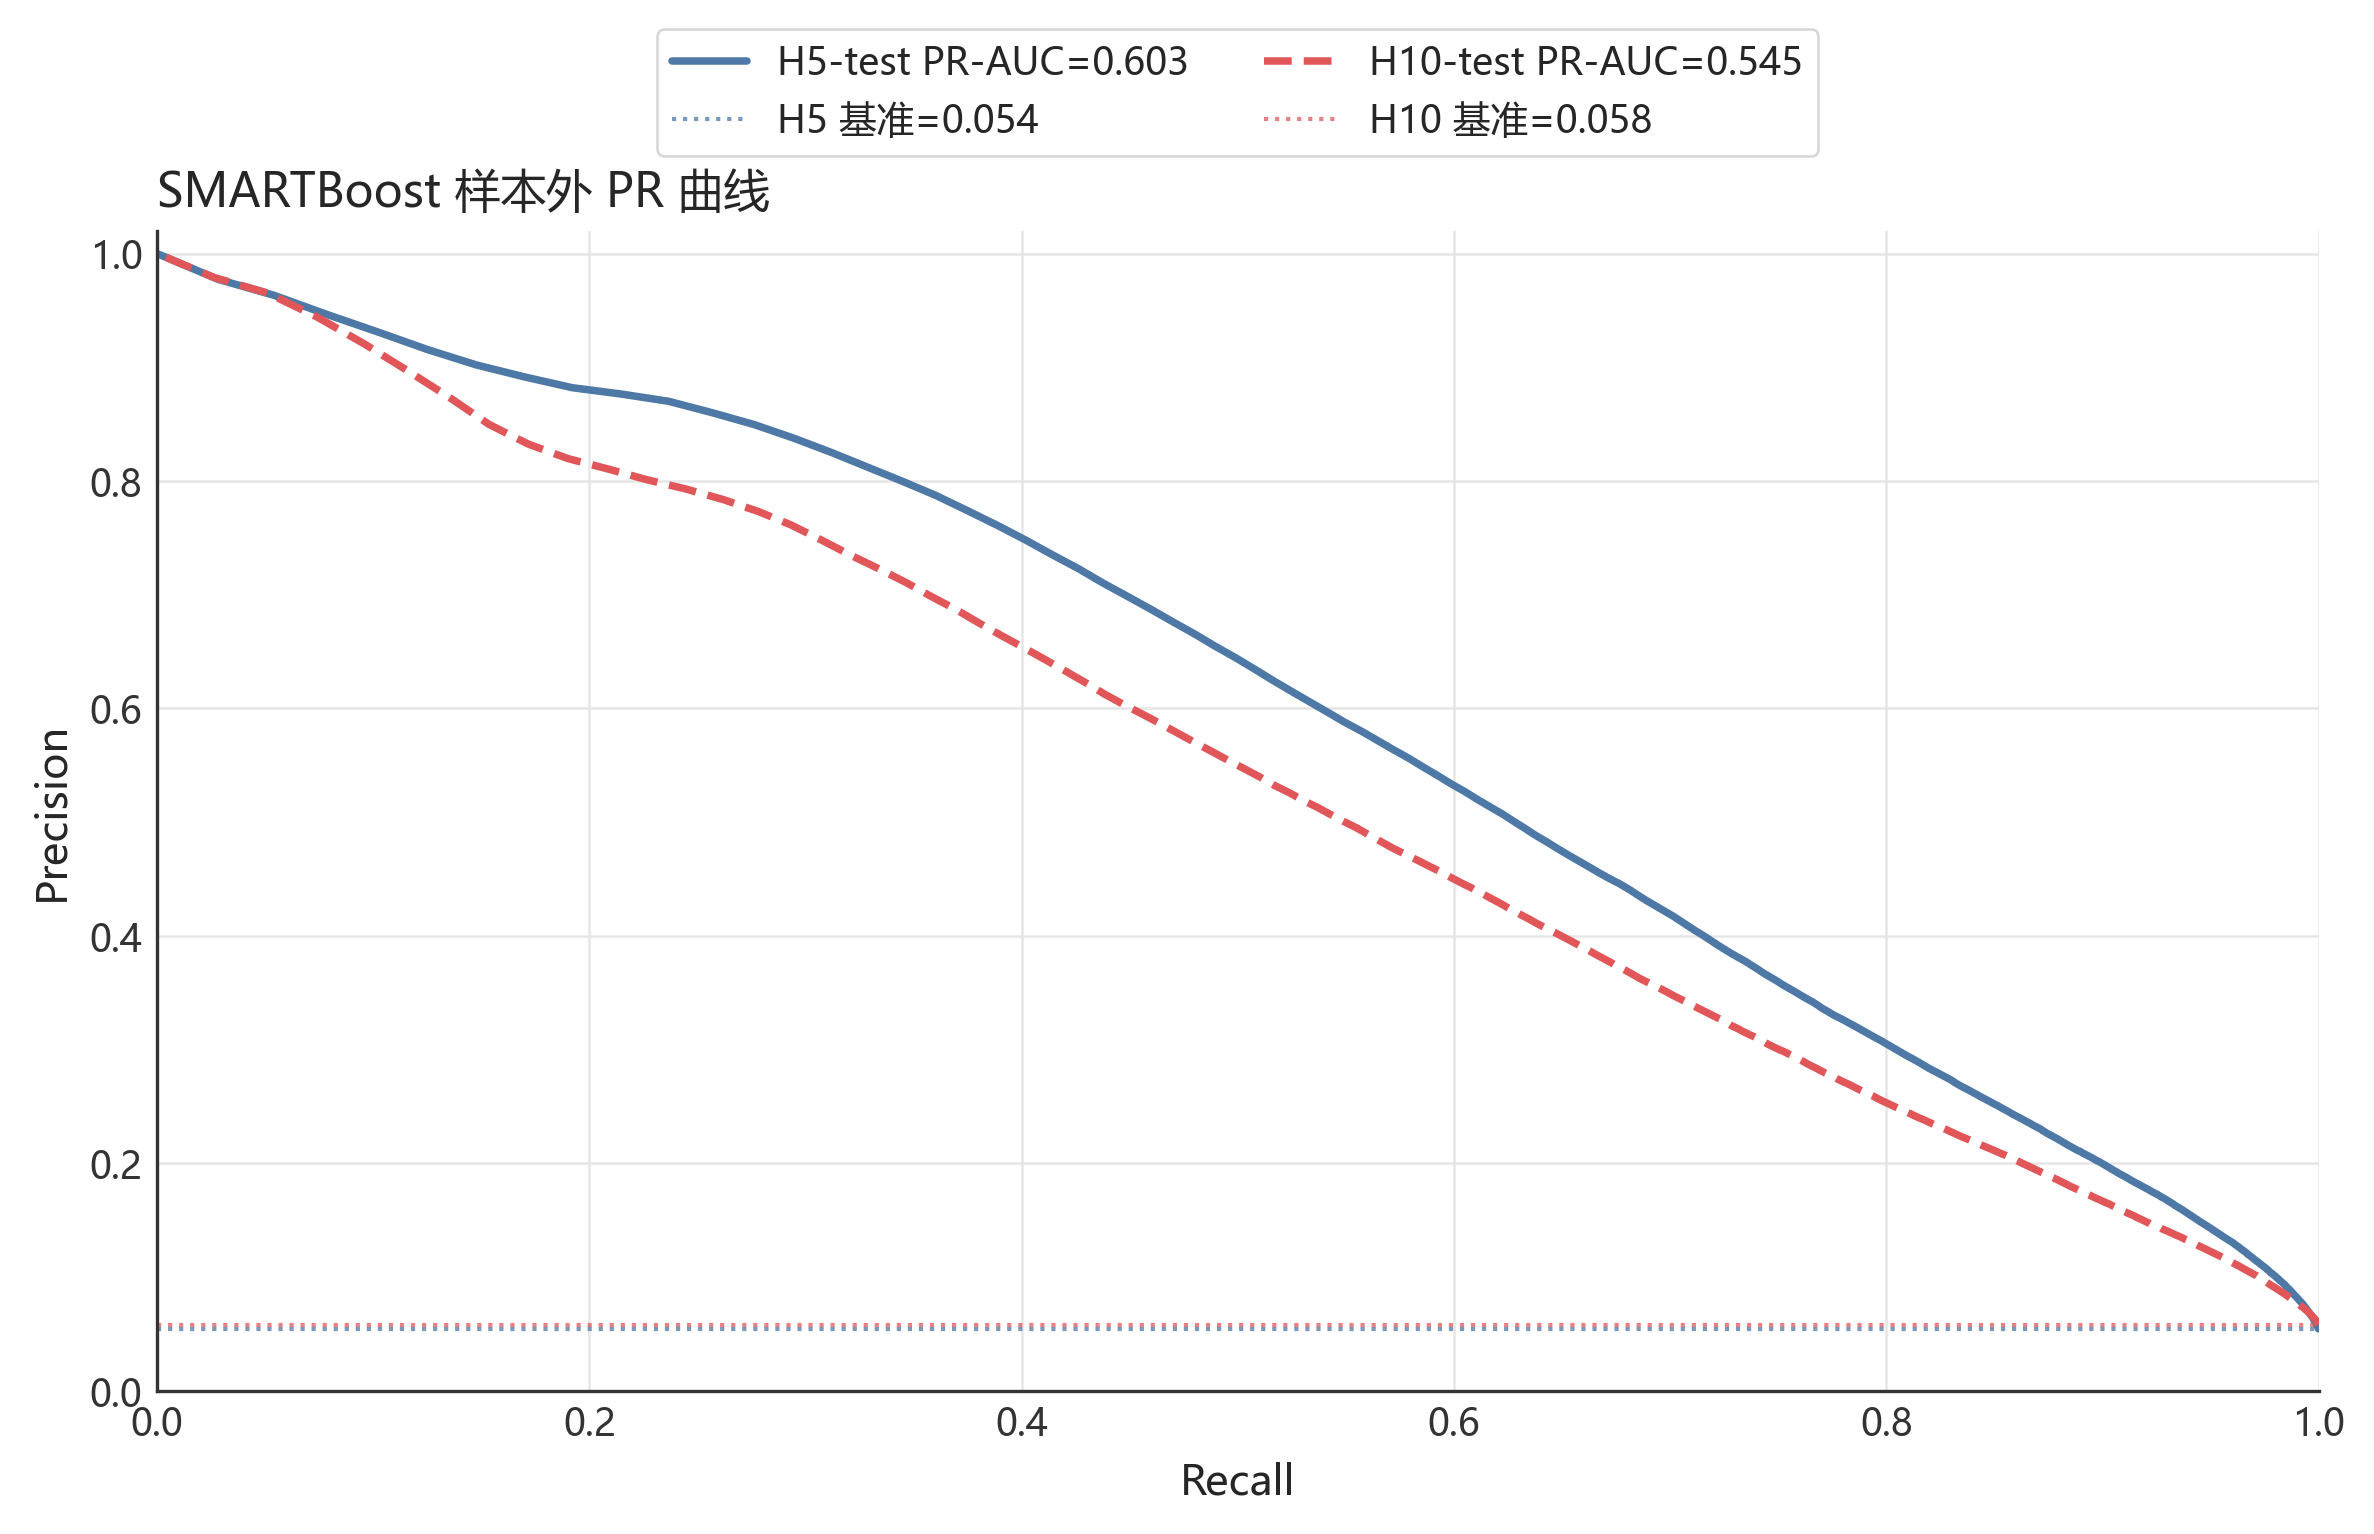
\includegraphics[width=0.78\linewidth,height=0.35\textheight,keepaspectratio]{figures/fig_sb_pr.png}
    \captionof{figure}{SMARTBoost 样本外 PR 曲线}
    \label{fig:sb-pr}
\endgroup
\end{center}

图中的水平基准线为对应样本的事件发生率。PR 曲线在整个精确率—召回率空间中均高于事件基准线，H5 曲线整体优于 H10，与表 \ref{tab:smartboost-metrics} 的结论一致。PR 曲线在较宽的召回率区间内持续高于水平基准线，表明模型不仅仅在极少数极端高风险样本上表现出色，并且可以在多个精确率—召回率权衡水平下保持一定排序优势。图 \ref{fig:sb-top5} 进一步考察预测概率最高的 Top 5\% 样本中真实压力事件的发生率，以更直观的形式展示模型的高风险排序能力。

\begin{center}
\begingroup
\captionsetup{type=figure}
    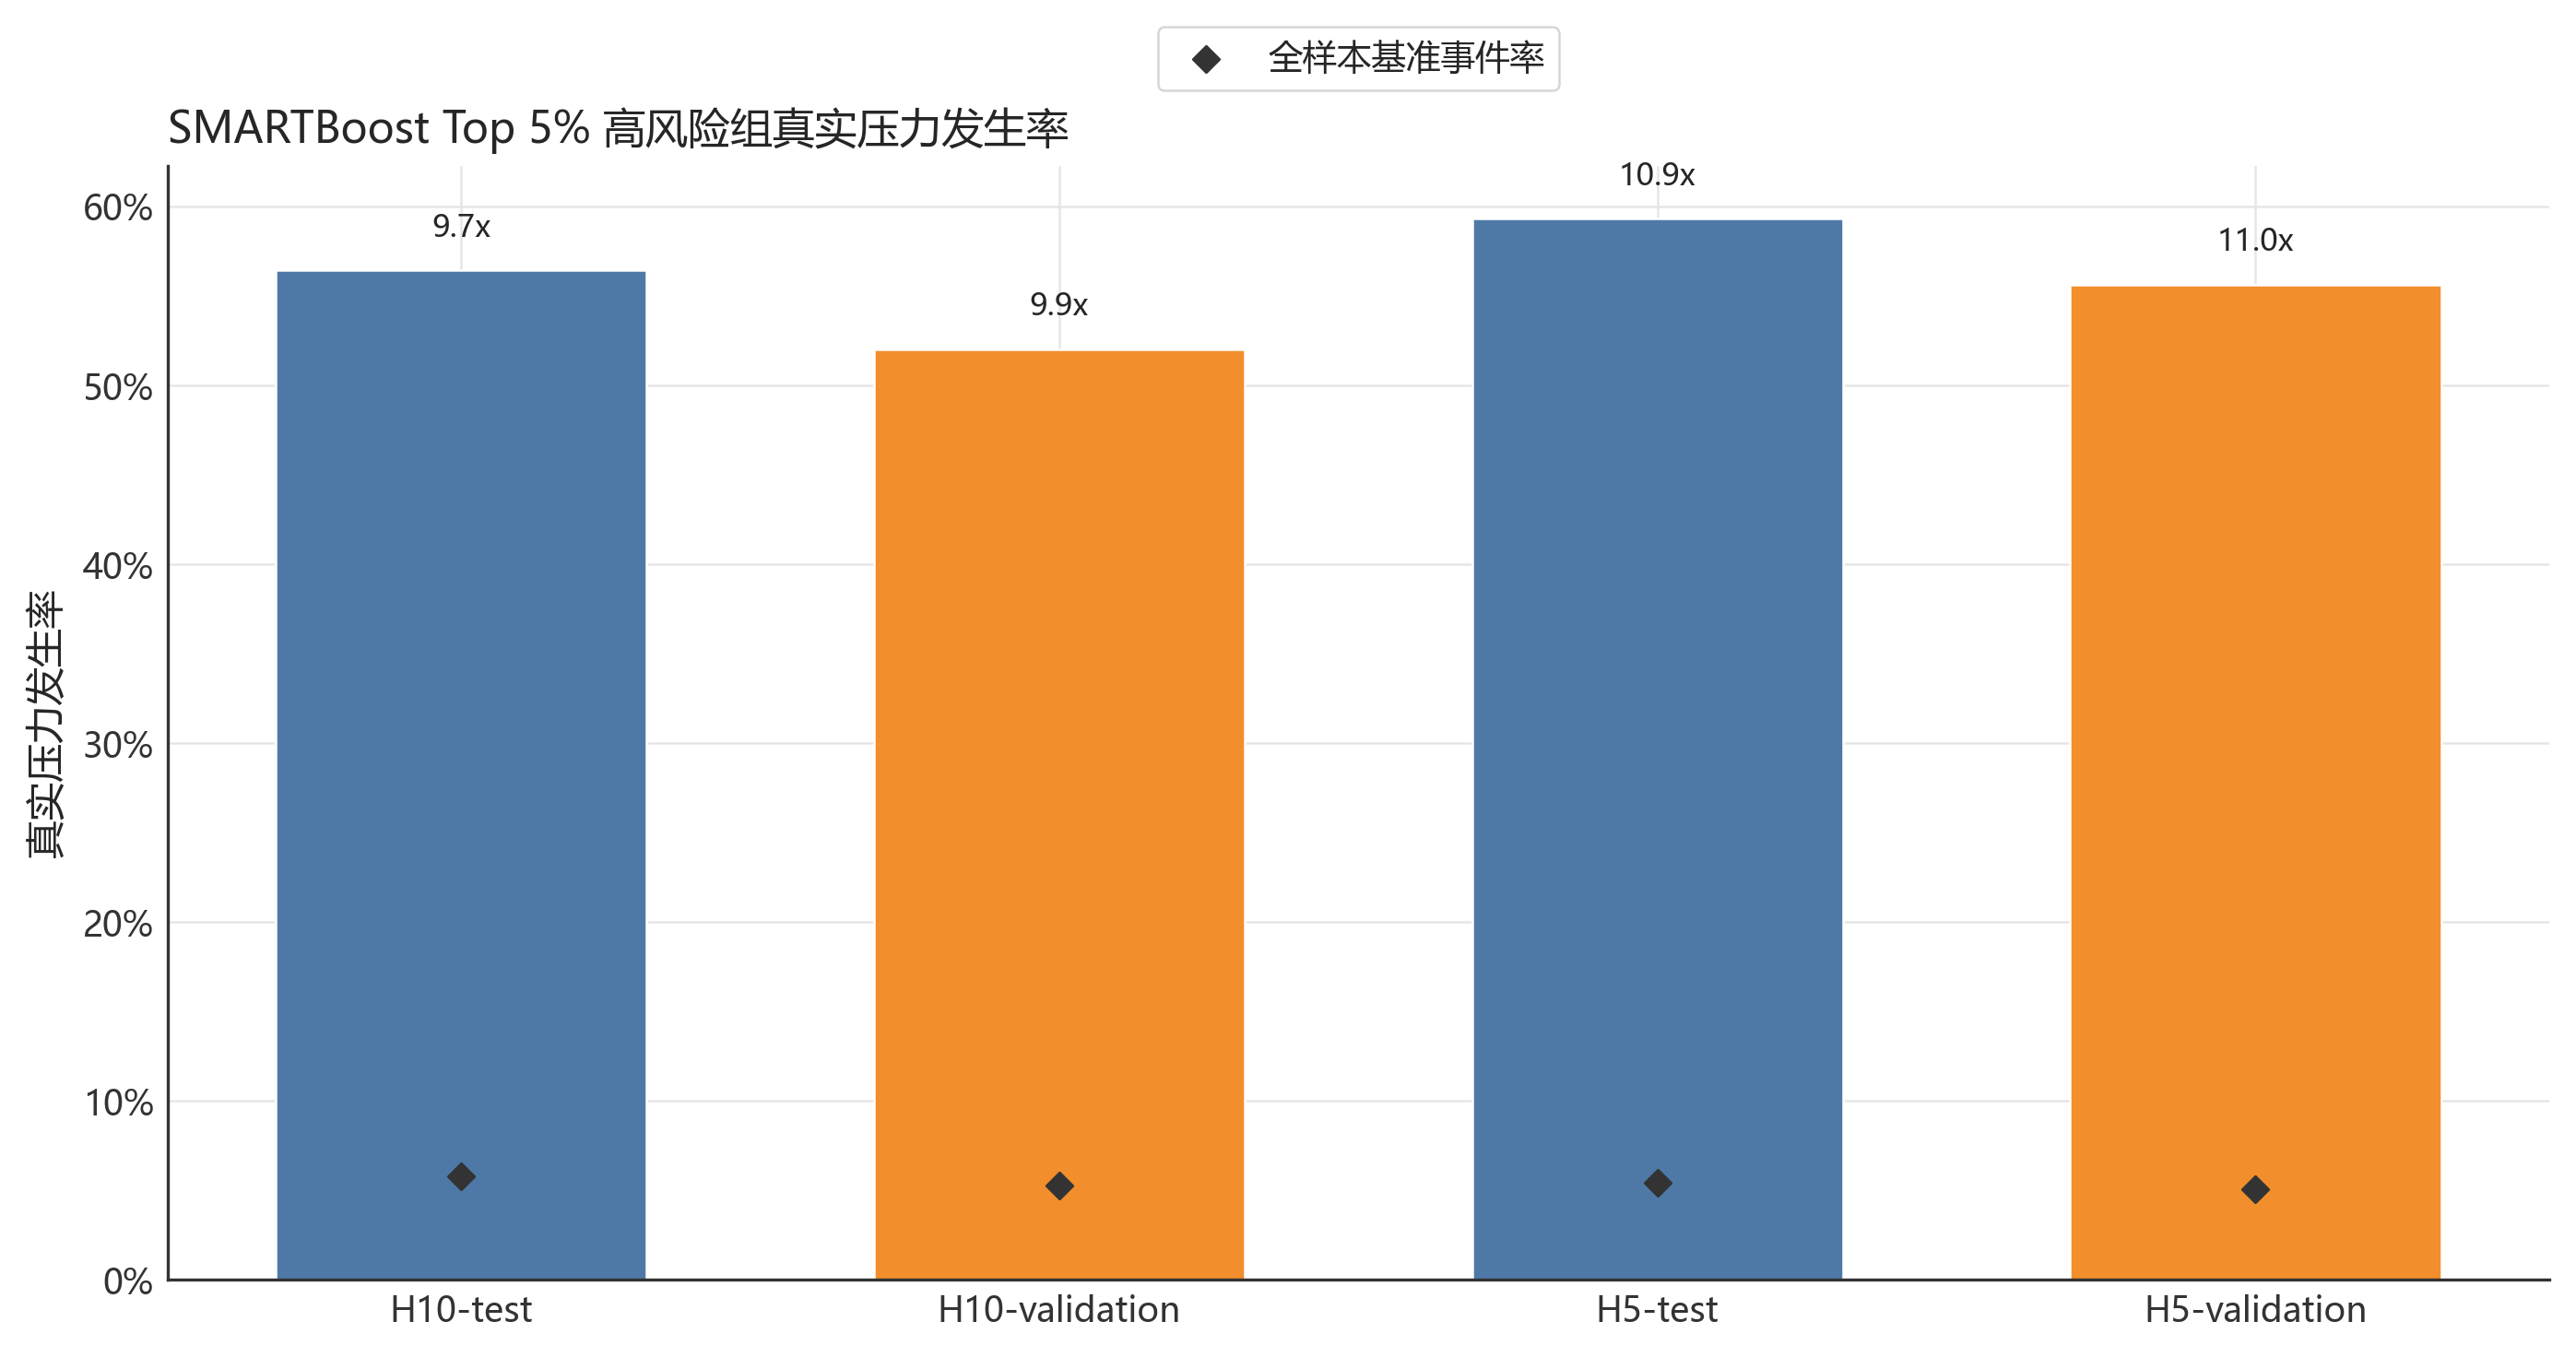
\includegraphics[width=0.78\linewidth,height=0.32\textheight,keepaspectratio]{figures/fig_sb_top5.png}
    \captionof{figure}{SMARTBoost Top 5\% 高风险组真实压力发生率}
    \label{fig:sb-top5}
\endgroup
\end{center}

图中柱状图对应验证集/测试集与 H5/H10 组合下的 Top 5\% 命中率，菱形标记为样本整体事件率。Top 5\% 高风险组中的真实压力发生率约为样本整体事件率的 10 倍，提升倍数约为 10。这是本文最直观的预警能力证据：模型能够将有限的预警资源集中到最可能发生压力的少数样本上。

为检验上述结论是否只依赖 Top 5\% 这一单一阈值，表 \ref{tab:smartboost-topk} 进一步报告测试集中从 Top 1\% 到 Top 20\% 各高风险分组的命中率与提升倍数。

\begin{center}
\begingroup
\captionsetup{type=table}
\begin{minipage}{\textwidth}
\centering
\captionof{table}{SMARTBoost 测试集高风险组真实压力发生率与提升倍数}
\label{tab:smartboost-topk}
\small
\begin{threeparttable}
\begin{tabular}{lrrr}
\toprule
目标 & 高风险组 & 真实压力发生率 & 提升倍数（lift） \\
\midrule
H10 & 1\% & 85.71\% & 14.77 \\
H10 & 5\% & 56.42\% & 9.72 \\
H10 & 10\% & 38.54\% & 6.64 \\
H10 & 20\% & 23.74\% & 4.09 \\
H5 & 1\% & 89.41\% & 16.43 \\
H5 & 5\% & 59.30\% & 10.90 \\
H5 & 10\% & 39.26\% & 7.21 \\
H5 & 20\% & 23.56\% & 4.33 \\
\bottomrule
\end{tabular}
\begin{tablenotes}[flushleft]
\footnotesize
\item 注：Top-$K$ 分组按预测风险从高到低排序得到；提升倍数为相对于测试集整体事件率的倍数。
\end{tablenotes}
\end{threeparttable}
\end{minipage}
\endgroup
\end{center}

从 Top 1\% 到 Top 20\% 的各高风险组均明显高于整体事件率；随覆盖比例扩大，提升倍数递减符合风险排序任务的一般规律。在实践层面，高风险分组的价值在于面对有限监测资源时，能够将重点预警集中于最可能发生压力的少数时间点；因此，提升度较总体分类准确率更能反映模型的实际预警价值。最后，图 \ref{fig:sb-partial} 展示核心变量的局部效应，用于解释主要特征如何影响预测概率。

\begin{center}
\begingroup
\captionsetup{type=figure}
    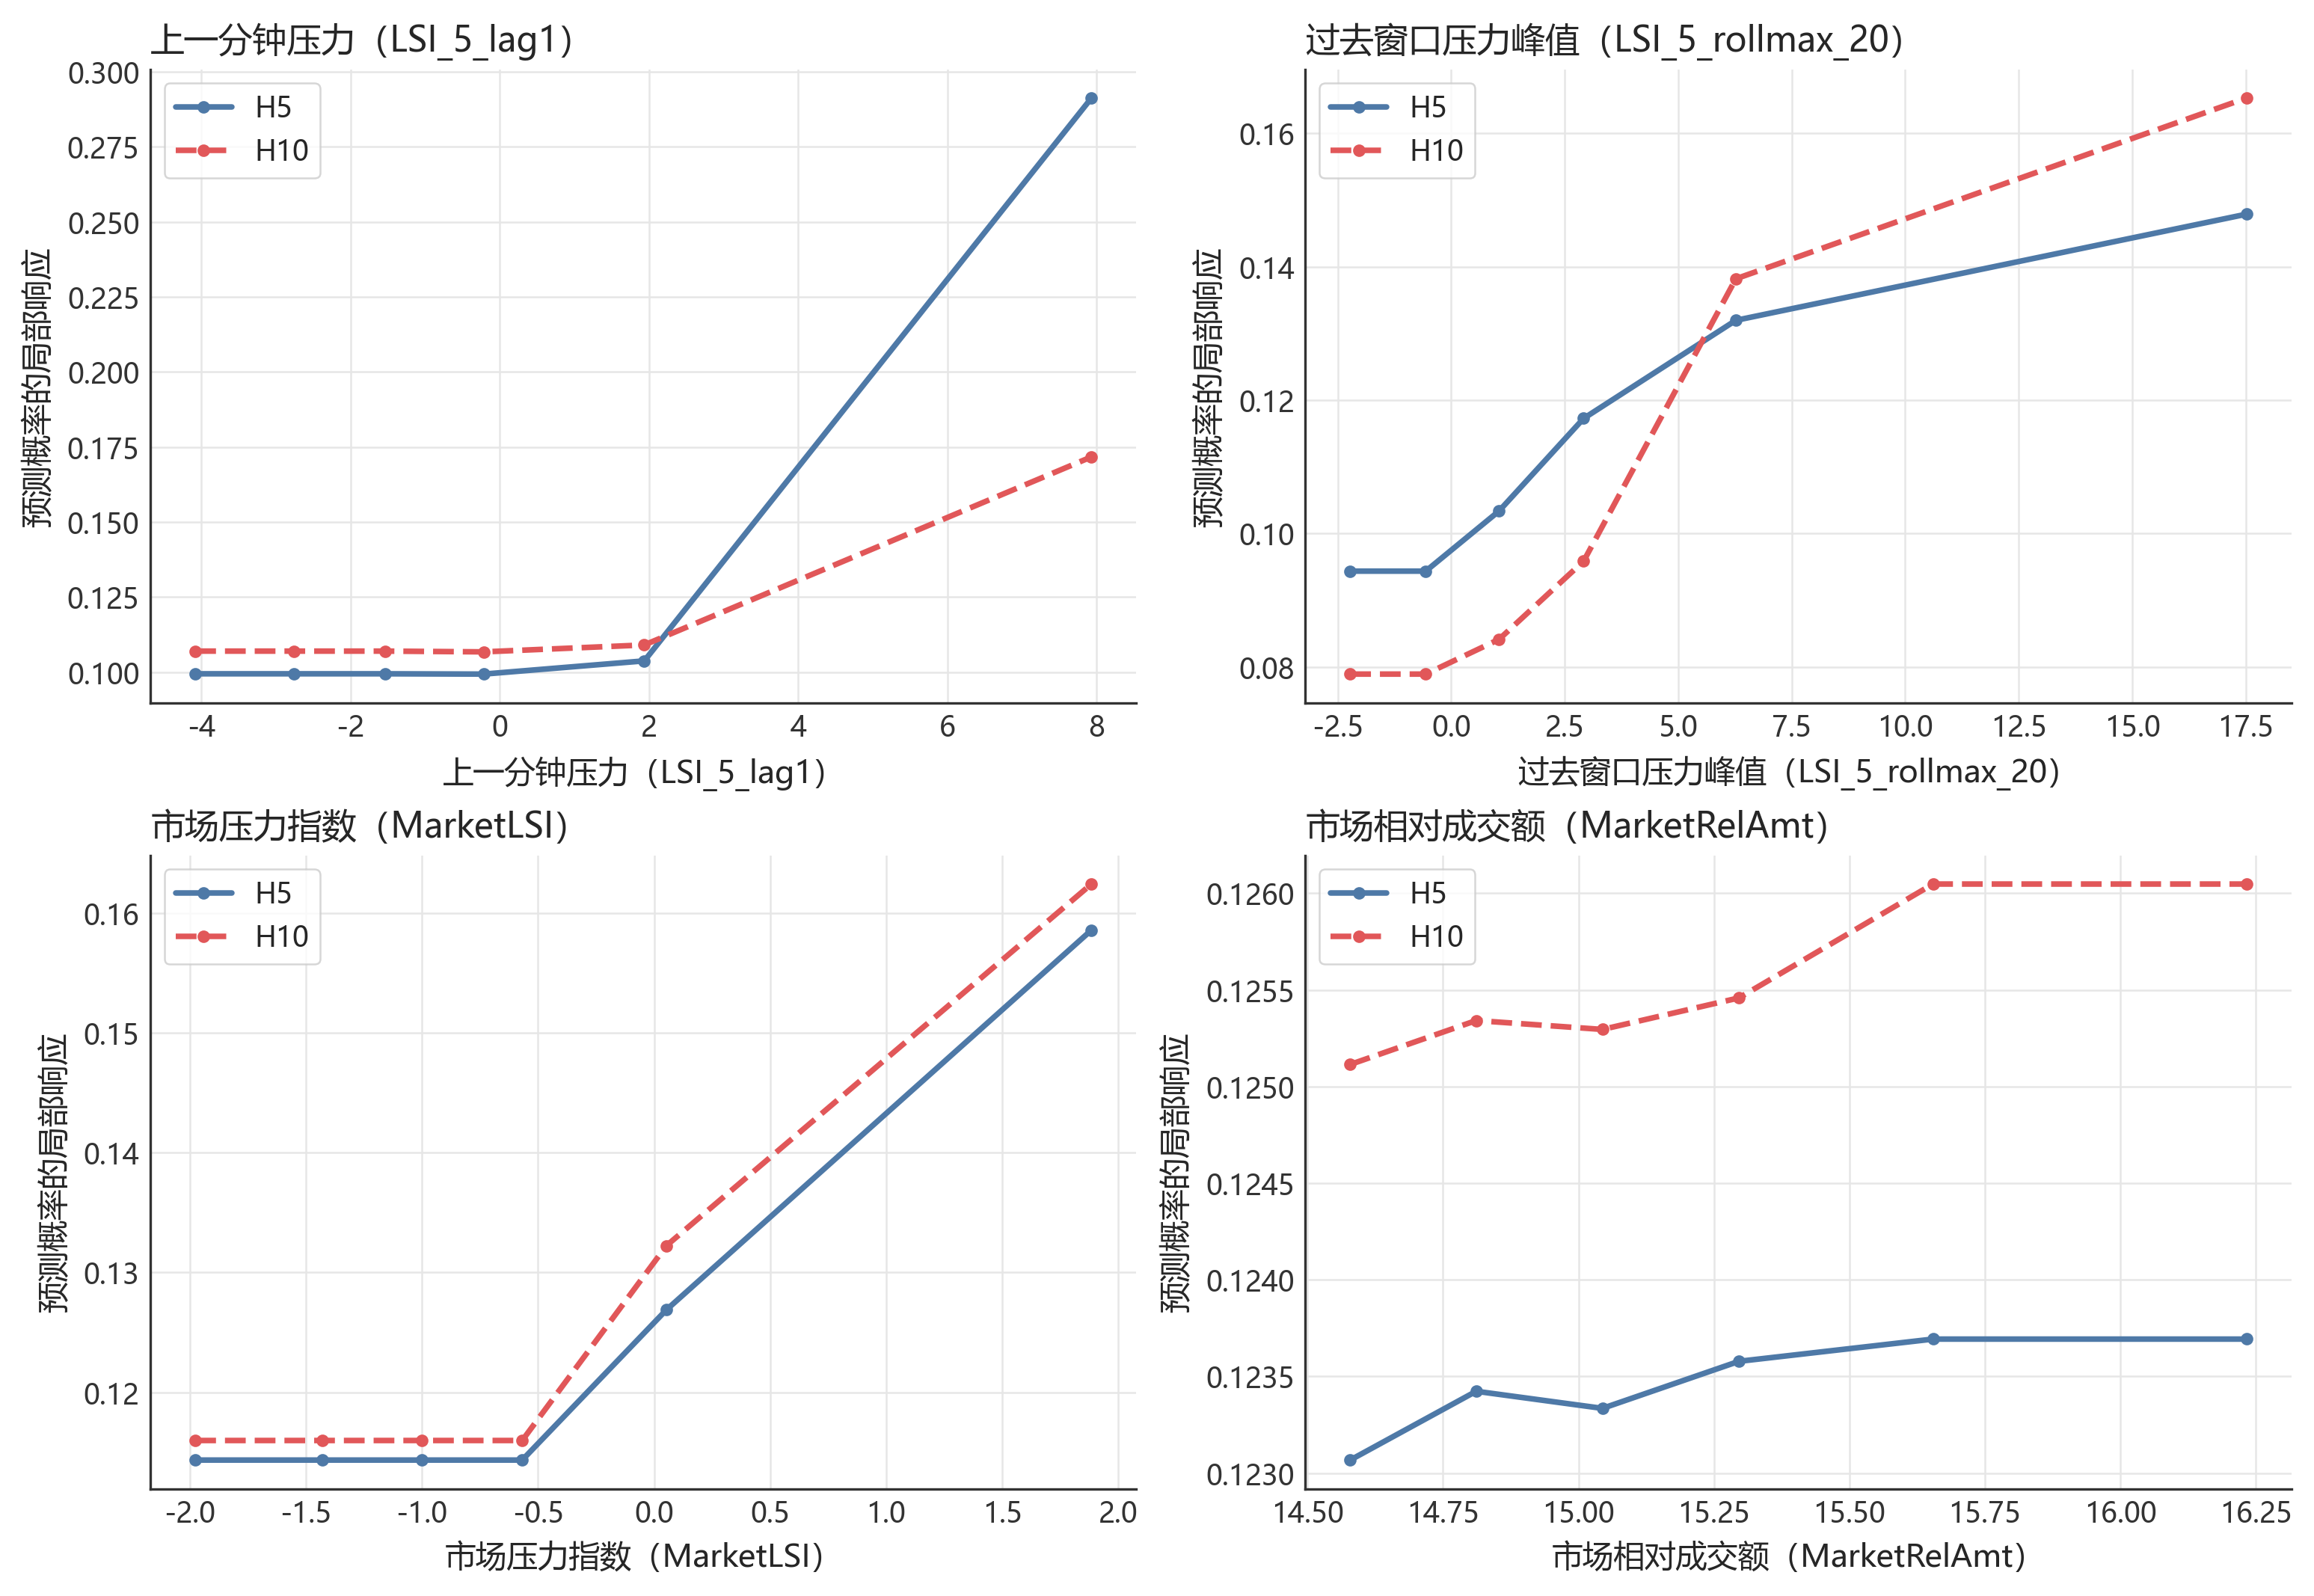
\includegraphics[width=0.82\linewidth,height=0.38\textheight,keepaspectratio]{figures/fig_sb_partial.png}
    \captionof{figure}{SMARTBoost 核心变量 Partial Effects}
    \label{fig:sb-partial}
\endgroup
\end{center}

图中横轴为特征取值，纵轴为预测概率的局部响应。局部效应显示，当前分钟压力、过去窗口压力峰值和市场压力指数升高时，预测压力概率整体增加；市场成交承接力降低时也对应更高的预警概率。这些方向与 LSI 构造中的经济直觉相一致，强化了变量经济含义与样本外预警结果之间的联系。局部效应与 LSI 指标的构造逻辑相吻合，增强了机器学习预警结果的经济解释性。

\begin{sloppypar}
为保证样本外预警检验的有效性，本文在预测特征矩阵中排除了 Stress\_H5、Stress\_H10、FutureMaxLSI、CrossStress 等由未来窗口或未来标签聚合得到的变量；滚动特征仅使用 $t$ 时点及以前的信息，训练、验证与测试样本按时间顺序划分。因此，SMARTBoost 的样本外表现可以解释为历史高频状态变量的预警能力，在此设定下，SMARTBoost 提供了第三层也是最直接的证据：分钟级历史状态变量能够对未来 H5/H10 压力事件形成有效的样本外高风险排序。
\end{sloppypar}


\subsection{三类证据链的综合解释}
\label{subsec:synthesis}

上述结果表明，RGARCH-CARR-SK、QVAR 与 SMARTBoost 分别从动态风险、尾部分位联动和样本外预测三个角度提供互补证据。RGARCH-CARR-SK 说明 MarketLSI 压力风险具有阶段性聚集结构，且风险路径对已实现压力测度的选择较为敏感；QVAR 进一步说明这种压力状态与市场收益、波动和成交承接变量之间存在尾部分位联动，且联动在高分位状态下更为显著；SMARTBoost 则在严格的样本外设定下验证，这些历史状态变量确实能够对未来压力事件形成有效的风险排序。

本文的最终回答是肯定的：A 股分钟级市场状态信息能够对未来 5 分钟和 10 分钟的短时流动性压力形成可验证的样本外预警。这一结论的解释范围包括三个方面：LSI 是基于成交后数据构造的代理型压力指标；QVAR 反映条件分位联动；SMARTBoost 用于未来压力事件排序预警。


% ============================================================
% 6 稳健性检验
% ============================================================
\section{稳健性检验}

为评估上述实证结论对研究设计选择的敏感性，本章从四个维度实施稳健性检验：标签阈值设定、RGARCH 已实现压力测度口径、QVAR 分位点与情景设定，以及 SMARTBoost 的 Top-$K$ 分组宽度。

\subsection{标签阈值稳健性}

基准设定以训练期第 90 百分位数作为压力标签阈值。阈值降低会提高事件发生率，阈值提高会使压力事件更稀有；若模型的预警能力高度依赖这一特定阈值，则在 85\% 和 95\% 分位阈值下，PR-AUC、Top 5\% 命中率和提升倍数应出现明显波动。图 \ref{fig:robust-label} 分别报告训练期 85\%、90\% 和 95\% 分位阈值下的 PR-AUC 与 Top 5\% 提升倍数，用于检验样本外预警结论是否依赖单一标签阈值。

\begin{center}
\begingroup
\captionsetup{type=figure}
    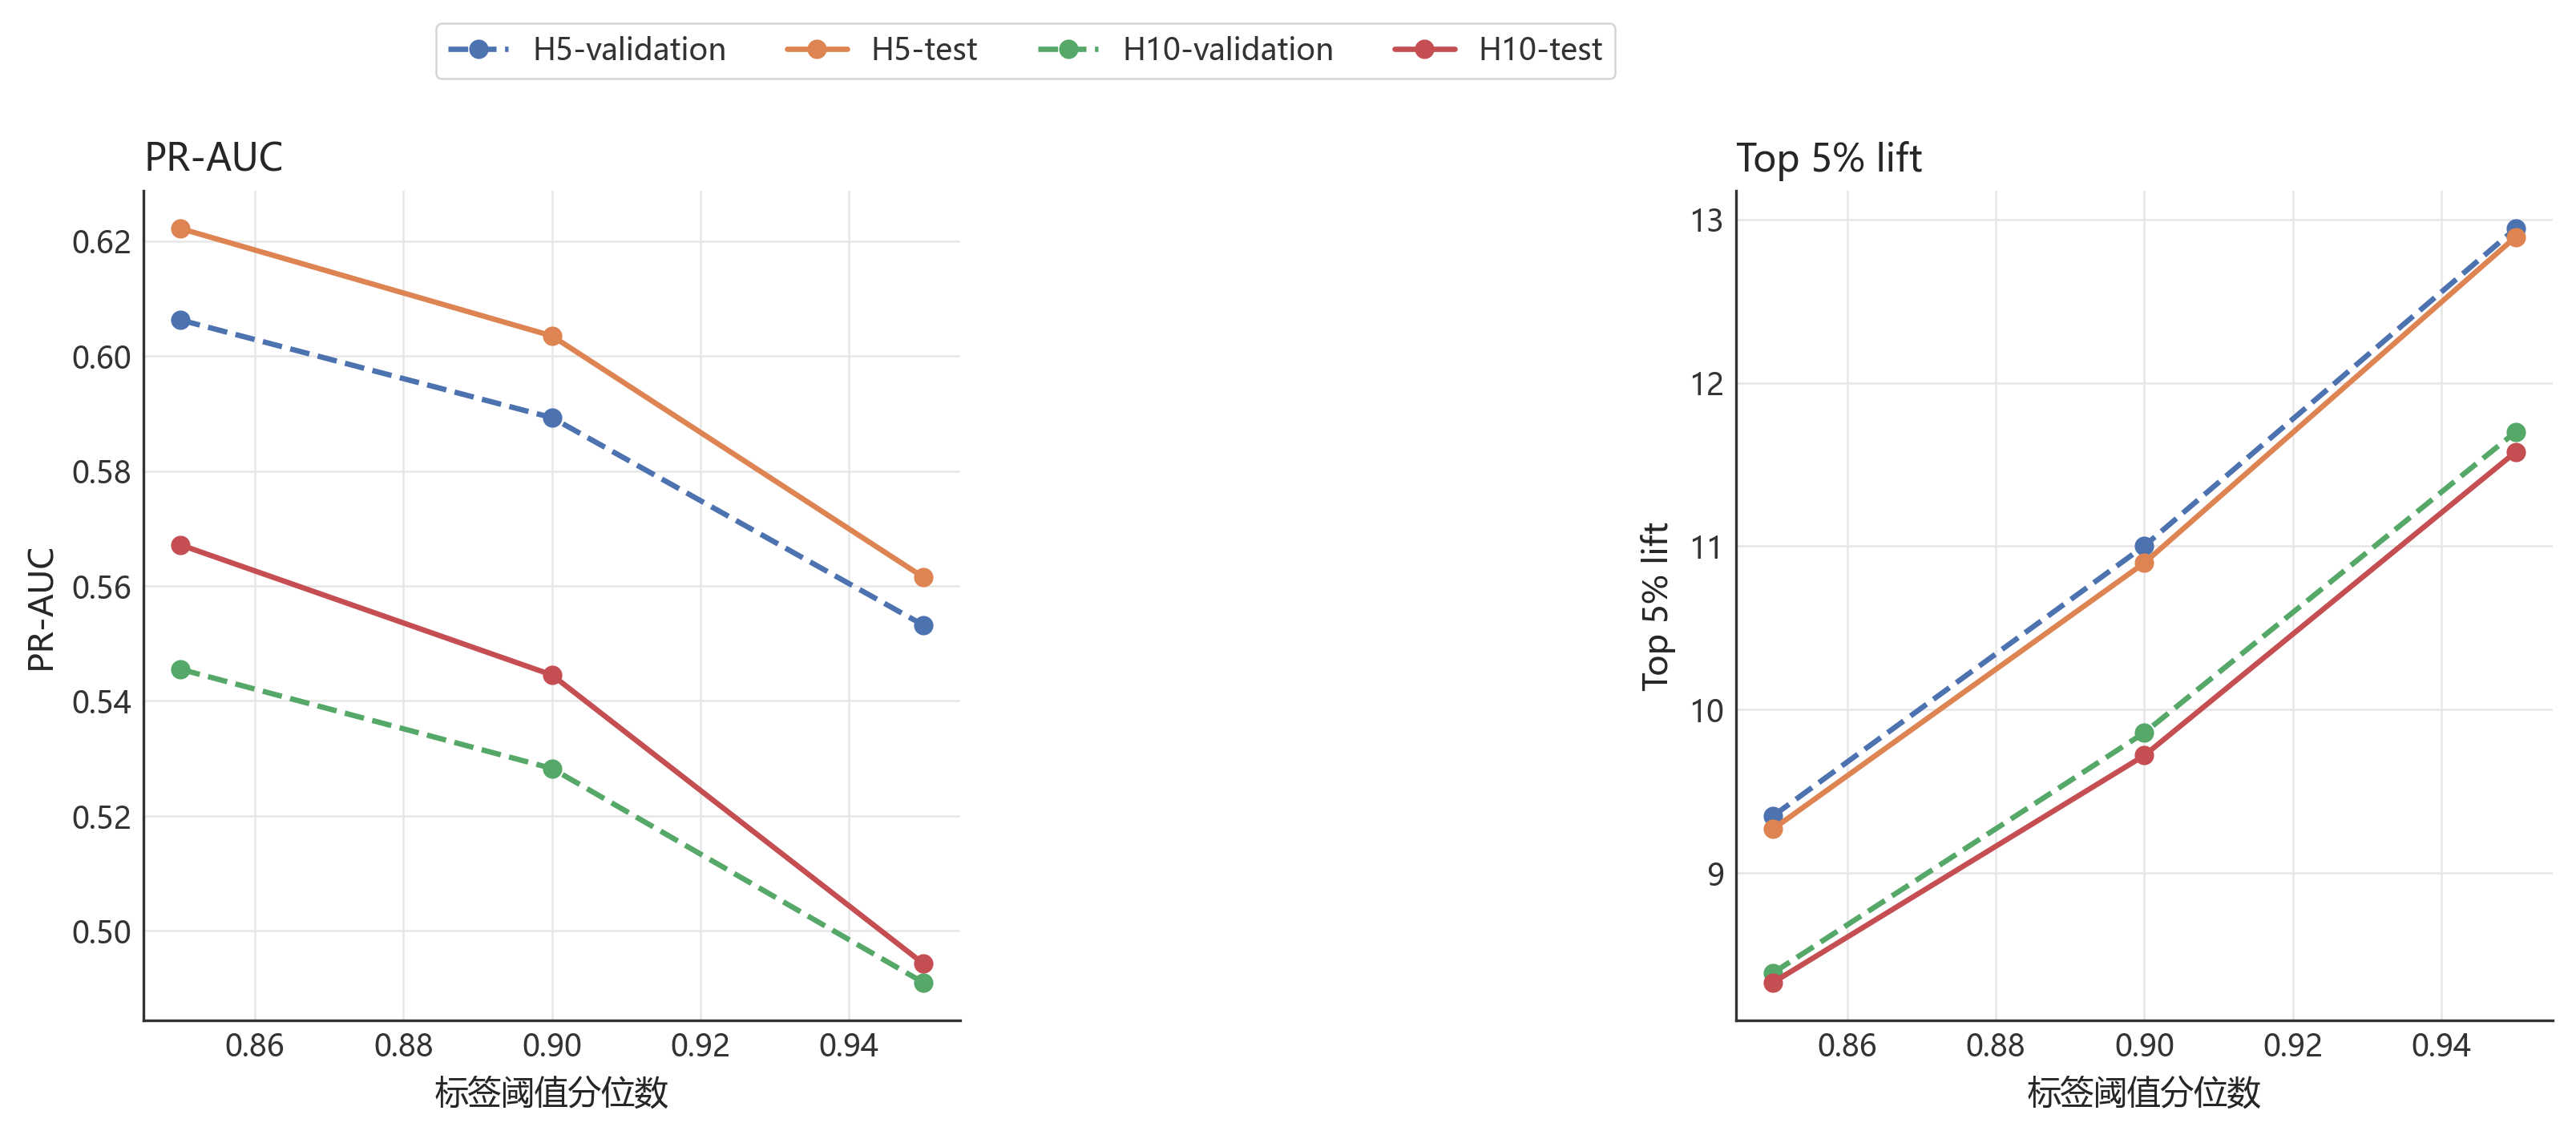
\includegraphics[width=0.82\textwidth]{figures/fig_robust_label_threshold.png}
    \captionof{figure}{标签阈值变化下的 SMARTBoost 样本外预警表现}
    \label{fig:robust-label}
\endgroup
\end{center}

虽然不同阈值下事件基准率和 PR-AUC 的绝对水平存在差异，但高风险组相对于基准事件率的提升倍数变化方向保持一致，说明模型的核心高风险排序结论具有跨阈值稳健性。

\Needspace{8\baselineskip}
\subsection{RGARCH 已实现压力测度稳健性}

正文表 \ref{tab:rgarch-loss} 已比较 RV、RBV、MedRV 与 RMAD 四类测度的样本外损失；图 \ref{fig:rgarch-realized-dist} 进一步展示四类测度的标准化分布形态差异，以理解损失差异背后的统计机制。

\begin{center}
\begingroup
\captionsetup{type=figure}
    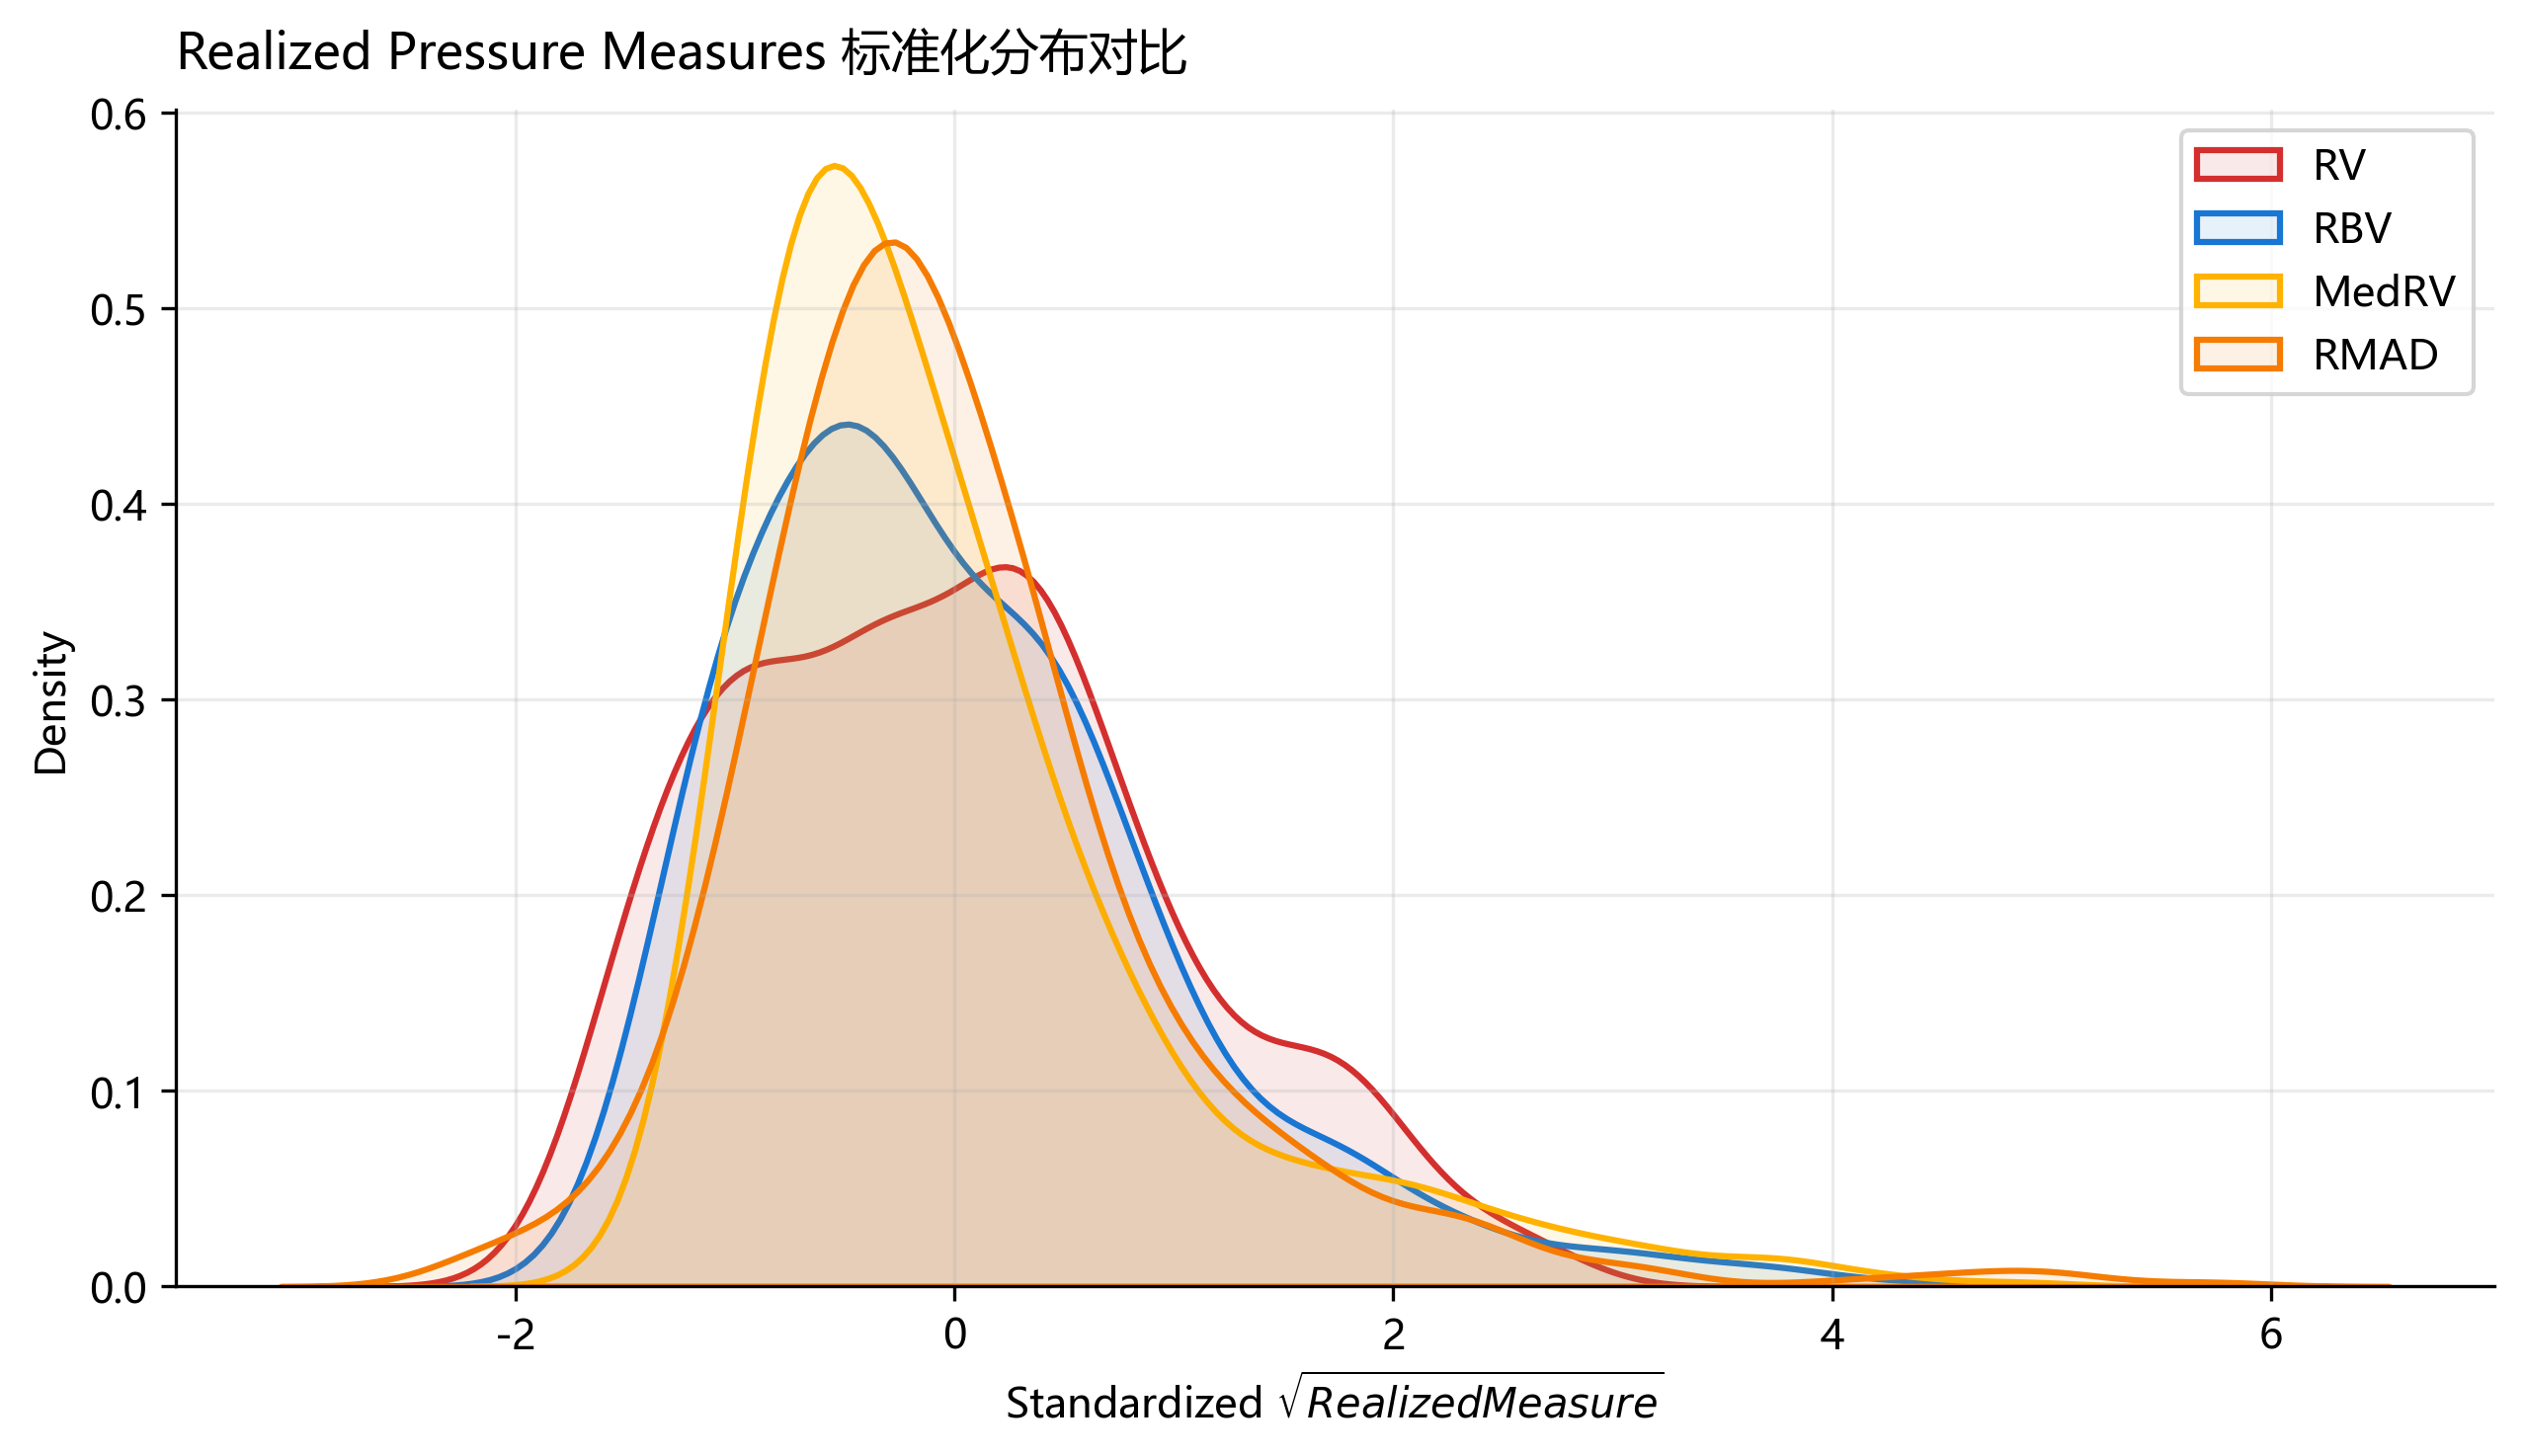
\includegraphics[width=0.78\linewidth,height=0.35\textheight,keepaspectratio]{figures/fig_rgarch_realized_measure_distribution_refined.png}
    \captionof{figure}{Realized pressure measures 标准化分布对比}
    \label{fig:rgarch-realized-dist}
\endgroup
\end{center}

不同已实现压力测度在刻画分布中心或尾部信息时具有不同统计属性，导致条件压力风险路径的估计误差出现差异。这一结果与高频波动文献中"不同已实现测度对微观结构噪声具有不同稳健性"的观点一致 \cite{andersen2003realized,barndorff2004bipower}。

\Needspace{8\baselineskip}
\subsection{QVAR 分位点与情景设定稳健性}

为避免单一预测步长或带符号响应方向造成解释偏误，本文进一步比较不同分位点下各情景的累计绝对响应强度。结果显示，$q=0.90$ 和 $q=0.95$ 尾部分位下，波动放大、成交收缩/流动性压力与复合压力情景的累计响应强度明显高于 $q=0.50$ 中位数状态，说明 MarketLSI 与市场状态变量之间的联动在尾部状态下更为敏感，支持 QVAR 的尾部分位异质性解释。

\begin{center}
\begingroup
\captionsetup{type=figure}
    
\includegraphics[width=0.78\linewidth,height=0.35\textheight,keepaspectratio]{../../05_outputs/figures/07_robustness/qvar_scenario_sensitivity/qvar_sensitivity_quantile_cum_abs_shock2.png}
    \captionof{figure}{不同分位点下 QVAR 情景响应累计强度比较}
    \label{fig:qvar-tail-summary}
\endgroup
\end{center}

\Needspace{8\baselineskip}
\subsection{SMARTBoost 特征组与 Top-K 稳健性}

图 \ref{fig:robust-topk} 展示从 Top 1\% 到 Top 20\% 不同宽度高风险分组下的真实压力发生率与提升倍数，以检验高风险排序结论对分组阈值选取的依赖程度。

\begin{center}
\begingroup
\captionsetup{type=figure}
    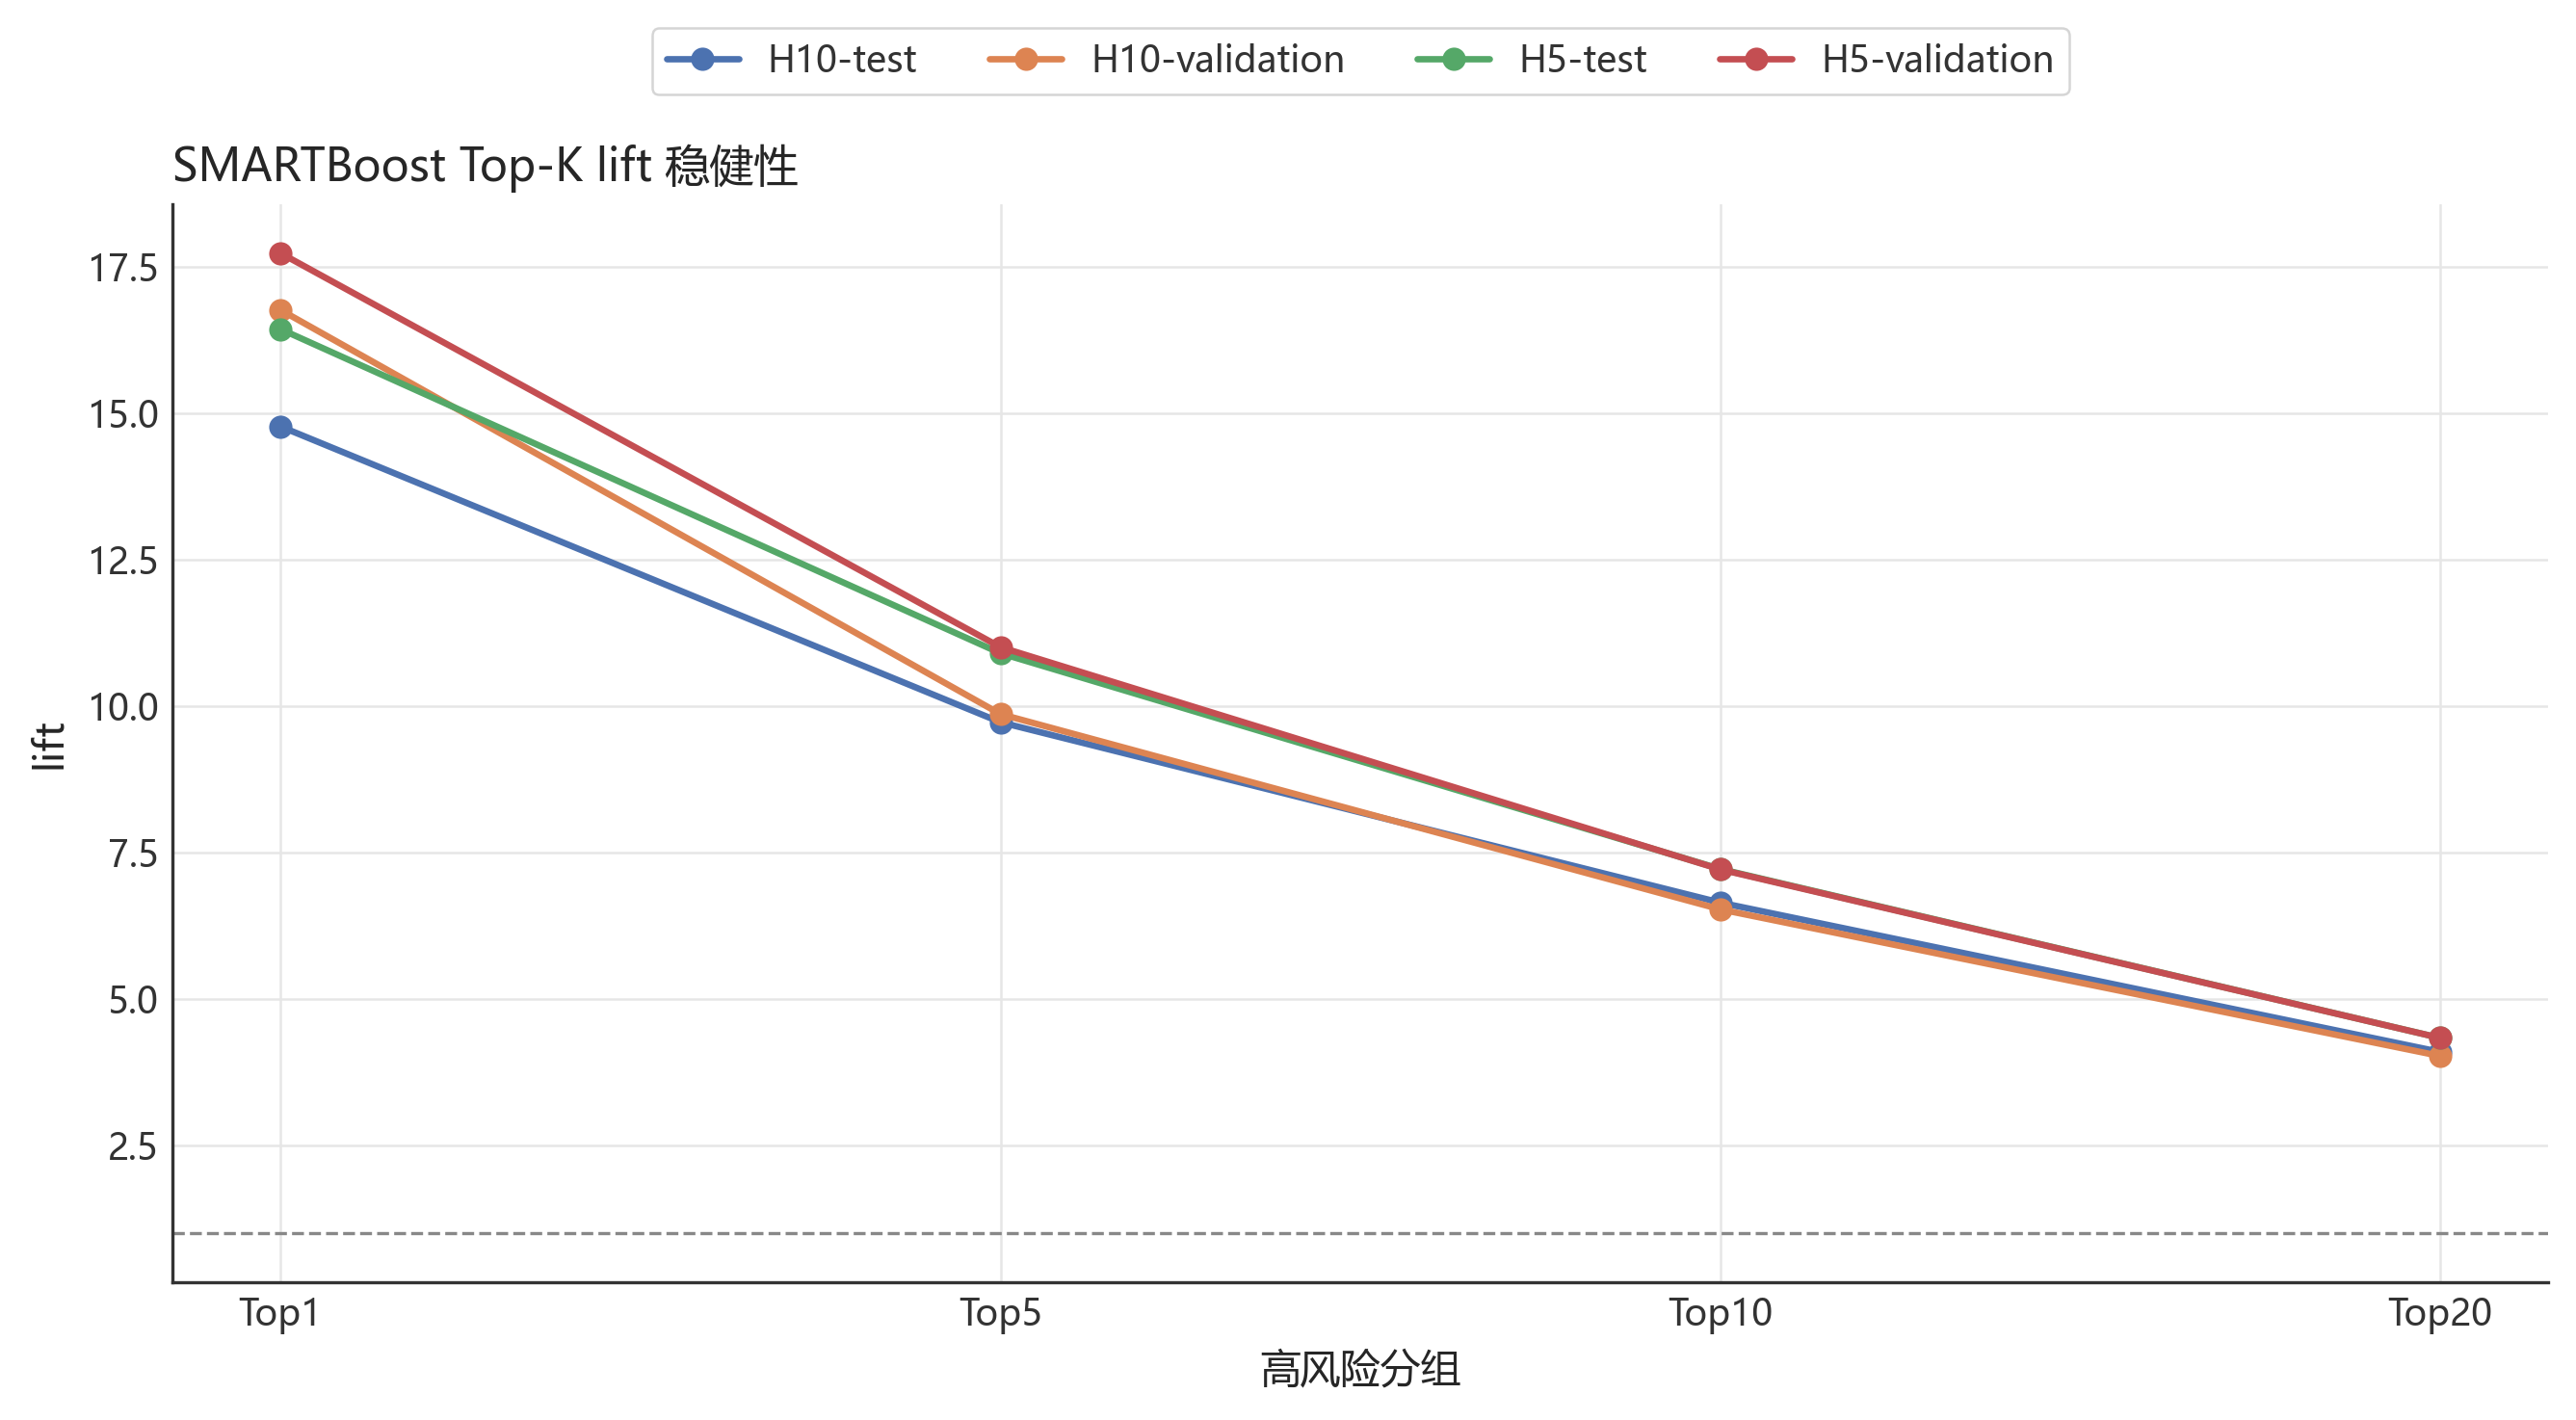
\includegraphics[width=0.78\linewidth,height=0.34\textheight,keepaspectratio]{figures/fig_robust_sb_topk.png}
    \captionof{figure}{不同高风险分组宽度下的真实压力发生率与 lift}
    \label{fig:robust-topk}
\endgroup
\end{center}

随着高风险分组从 Top 1\% 扩展至 Top 20\%，真实压力发生率和提升倍数逐步下降，但始终保持在整体事件基准率以上。这一结果说明 SMARTBoost 的高风险排序结论在不同分组宽度下均成立，并具有跨 Top-$K$ 阈值的一致性。Top-K 扩大时提升度自然下降，但只要各分组的真实压力发生率仍高于样本整体事件率，即说明模型的排序能力不只是单一阈值下的偶然结果，而具有跨分组的稳健性。




% ============================================================
% 7 结论与局限性
% ============================================================
\section{结论与局限性}

本文围绕"A 股分钟级市场状态信息能否预警未来 5 分钟和 10 分钟短时流动性压力"这一核心问题，构建了从高频压力指标构造、动态风险刻画、尾部分位传导到样本外机器学习预警的三层递进实证框架。在严格时间边界约束的样本外设定下，仅依靠 1 分钟 OHLCV 与成交额数据，即可对未来短时流动性压力事件形成具有统计意义的风险排序能力，本文对此给出肯定性回答。

具体而言，RGARCH-CARR-SK 结果表明 MarketLSI 压力风险具有阶段性聚集特征，同时揭示了风险路径对已实现压力测度口径的敏感性；动态峰度在本样本中基本稳定在正态基准附近，主要作为模型诊断信息。QVAR 结果显示，在尾部条件下市场压力、市场波动和成交承接变量之间的响应路径有别于中位数状态，且波动放大和复合压力情景的响应强度明显高于单独市场急跌情景，为后续特征选择提供了实证依据。SMARTBoost 结果进一步表明，在排除所有未来信息变量后，历史高频状态特征能够对测试集中的 H5 和 H10 压力事件形成有效的样本外高风险排序，Top 5\% 高风险组的提升倍数约达 10 倍，Top 1\% 组命中率超过 85\%。

本文存在以下局限。其一，LSI 和 MarketLSI 基于分钟 OHLCV 与成交额构造，是成交后市场状态的压力代理指标，若能进一步获取逐笔或盘口数据，压力测度的精度有望提升。其二，QVAR 压力测试是标准化情景模拟，主要用于比较条件响应路径，情景响应的强度和方向受估计误差及模型设定影响。其三，SMARTBoost 的样本外表现基于特定样本窗口（2023—2026 年），结论能否推广到更长历史时段、不同市场状态或其他 A 股子样本，仍有待进一步检验。其四，本文将 84 只证券聚合为市场层面指标，证券选取方式可能影响 MarketLSI 的代表性，在更广泛的全市场样本上复现结论是未来研究的自然延伸方向。

尽管如此，本文形成了从高频压力代理指标到动态风险刻画、尾部分位传导和样本外智能预警的完整实证链条，为基于常规可得高频数据的短时压力监测提供了一种具备可验证样本外能力的框架。

\FloatBarrier
\clearpage
\appendix

% ============================================================
% 附录图表
% ============================================================
\section{附录图表}

\subsection{描述性诊断补充图}

图 \ref{fig:app-event-rate} 补充报告压力事件率的月度时间变化，直观展示验证期和测试期事件率低于训练期的时间结构，支持正文关于样本外事件不平衡性的讨论。

\begin{figure}[!htbp]
    \centering
    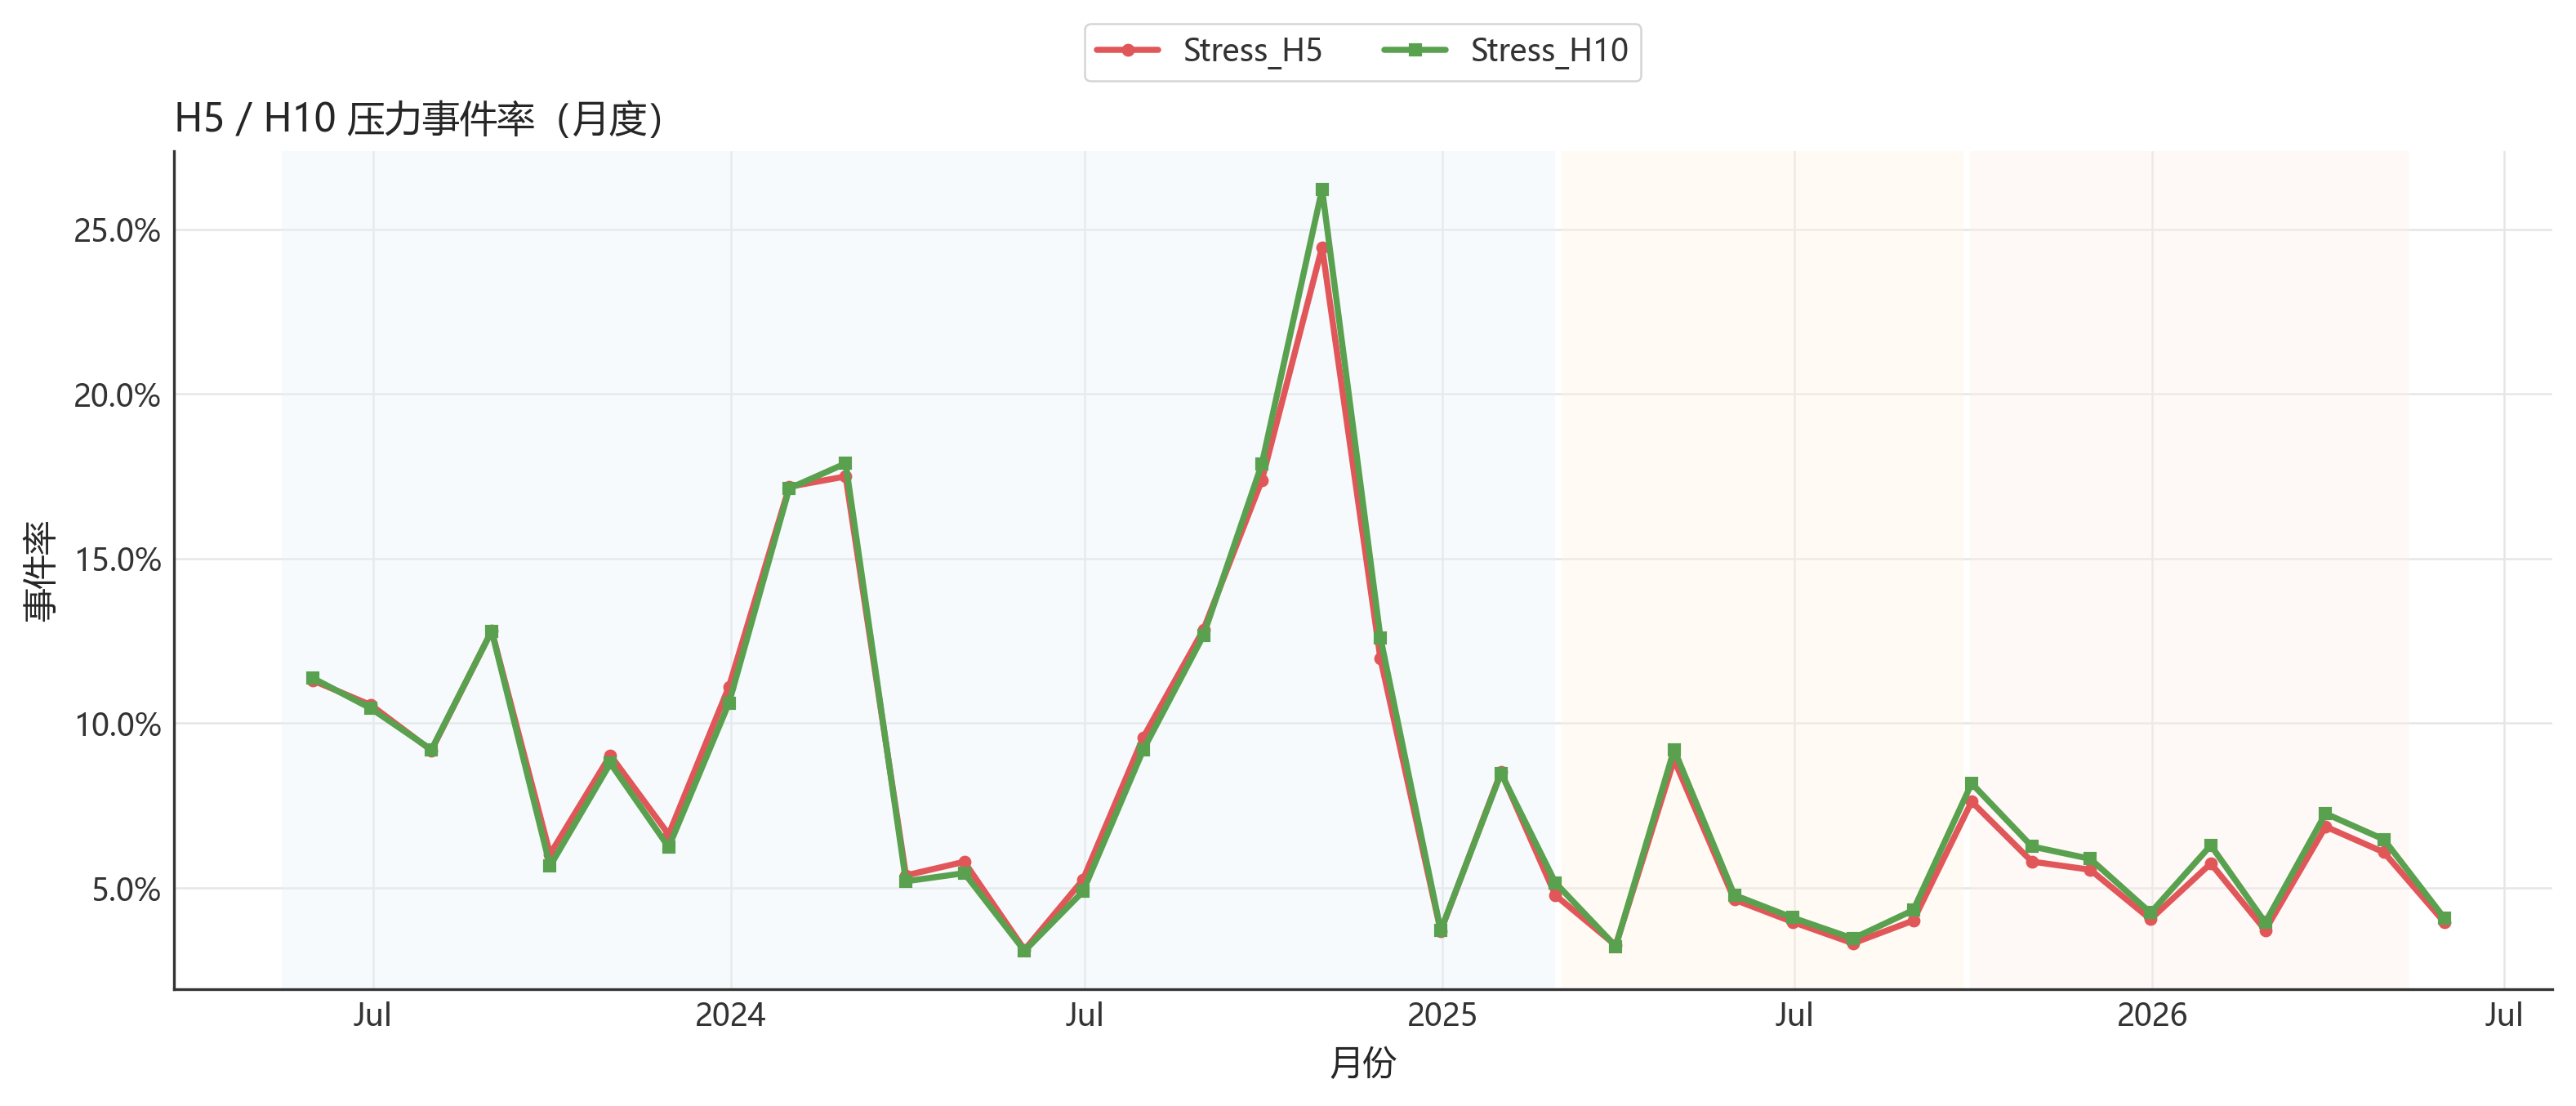
\includegraphics[width=0.88\textwidth]{figures/fig_event_rate.png}
    \caption{H5/H10 压力事件率月度时间变化}
    \label{fig:app-event-rate}
\end{figure}

图 \ref{fig:app-corr} 报告核心日度变量之间的线性相关结构，用于背景诊断。MarketLSI 与 H5/H10 压力标签之间的较高相关系数说明压力指标的构造具有一定的信息含量，线性相关结构主要用于描述变量共动。

\begin{figure}[!htbp]
    \centering
    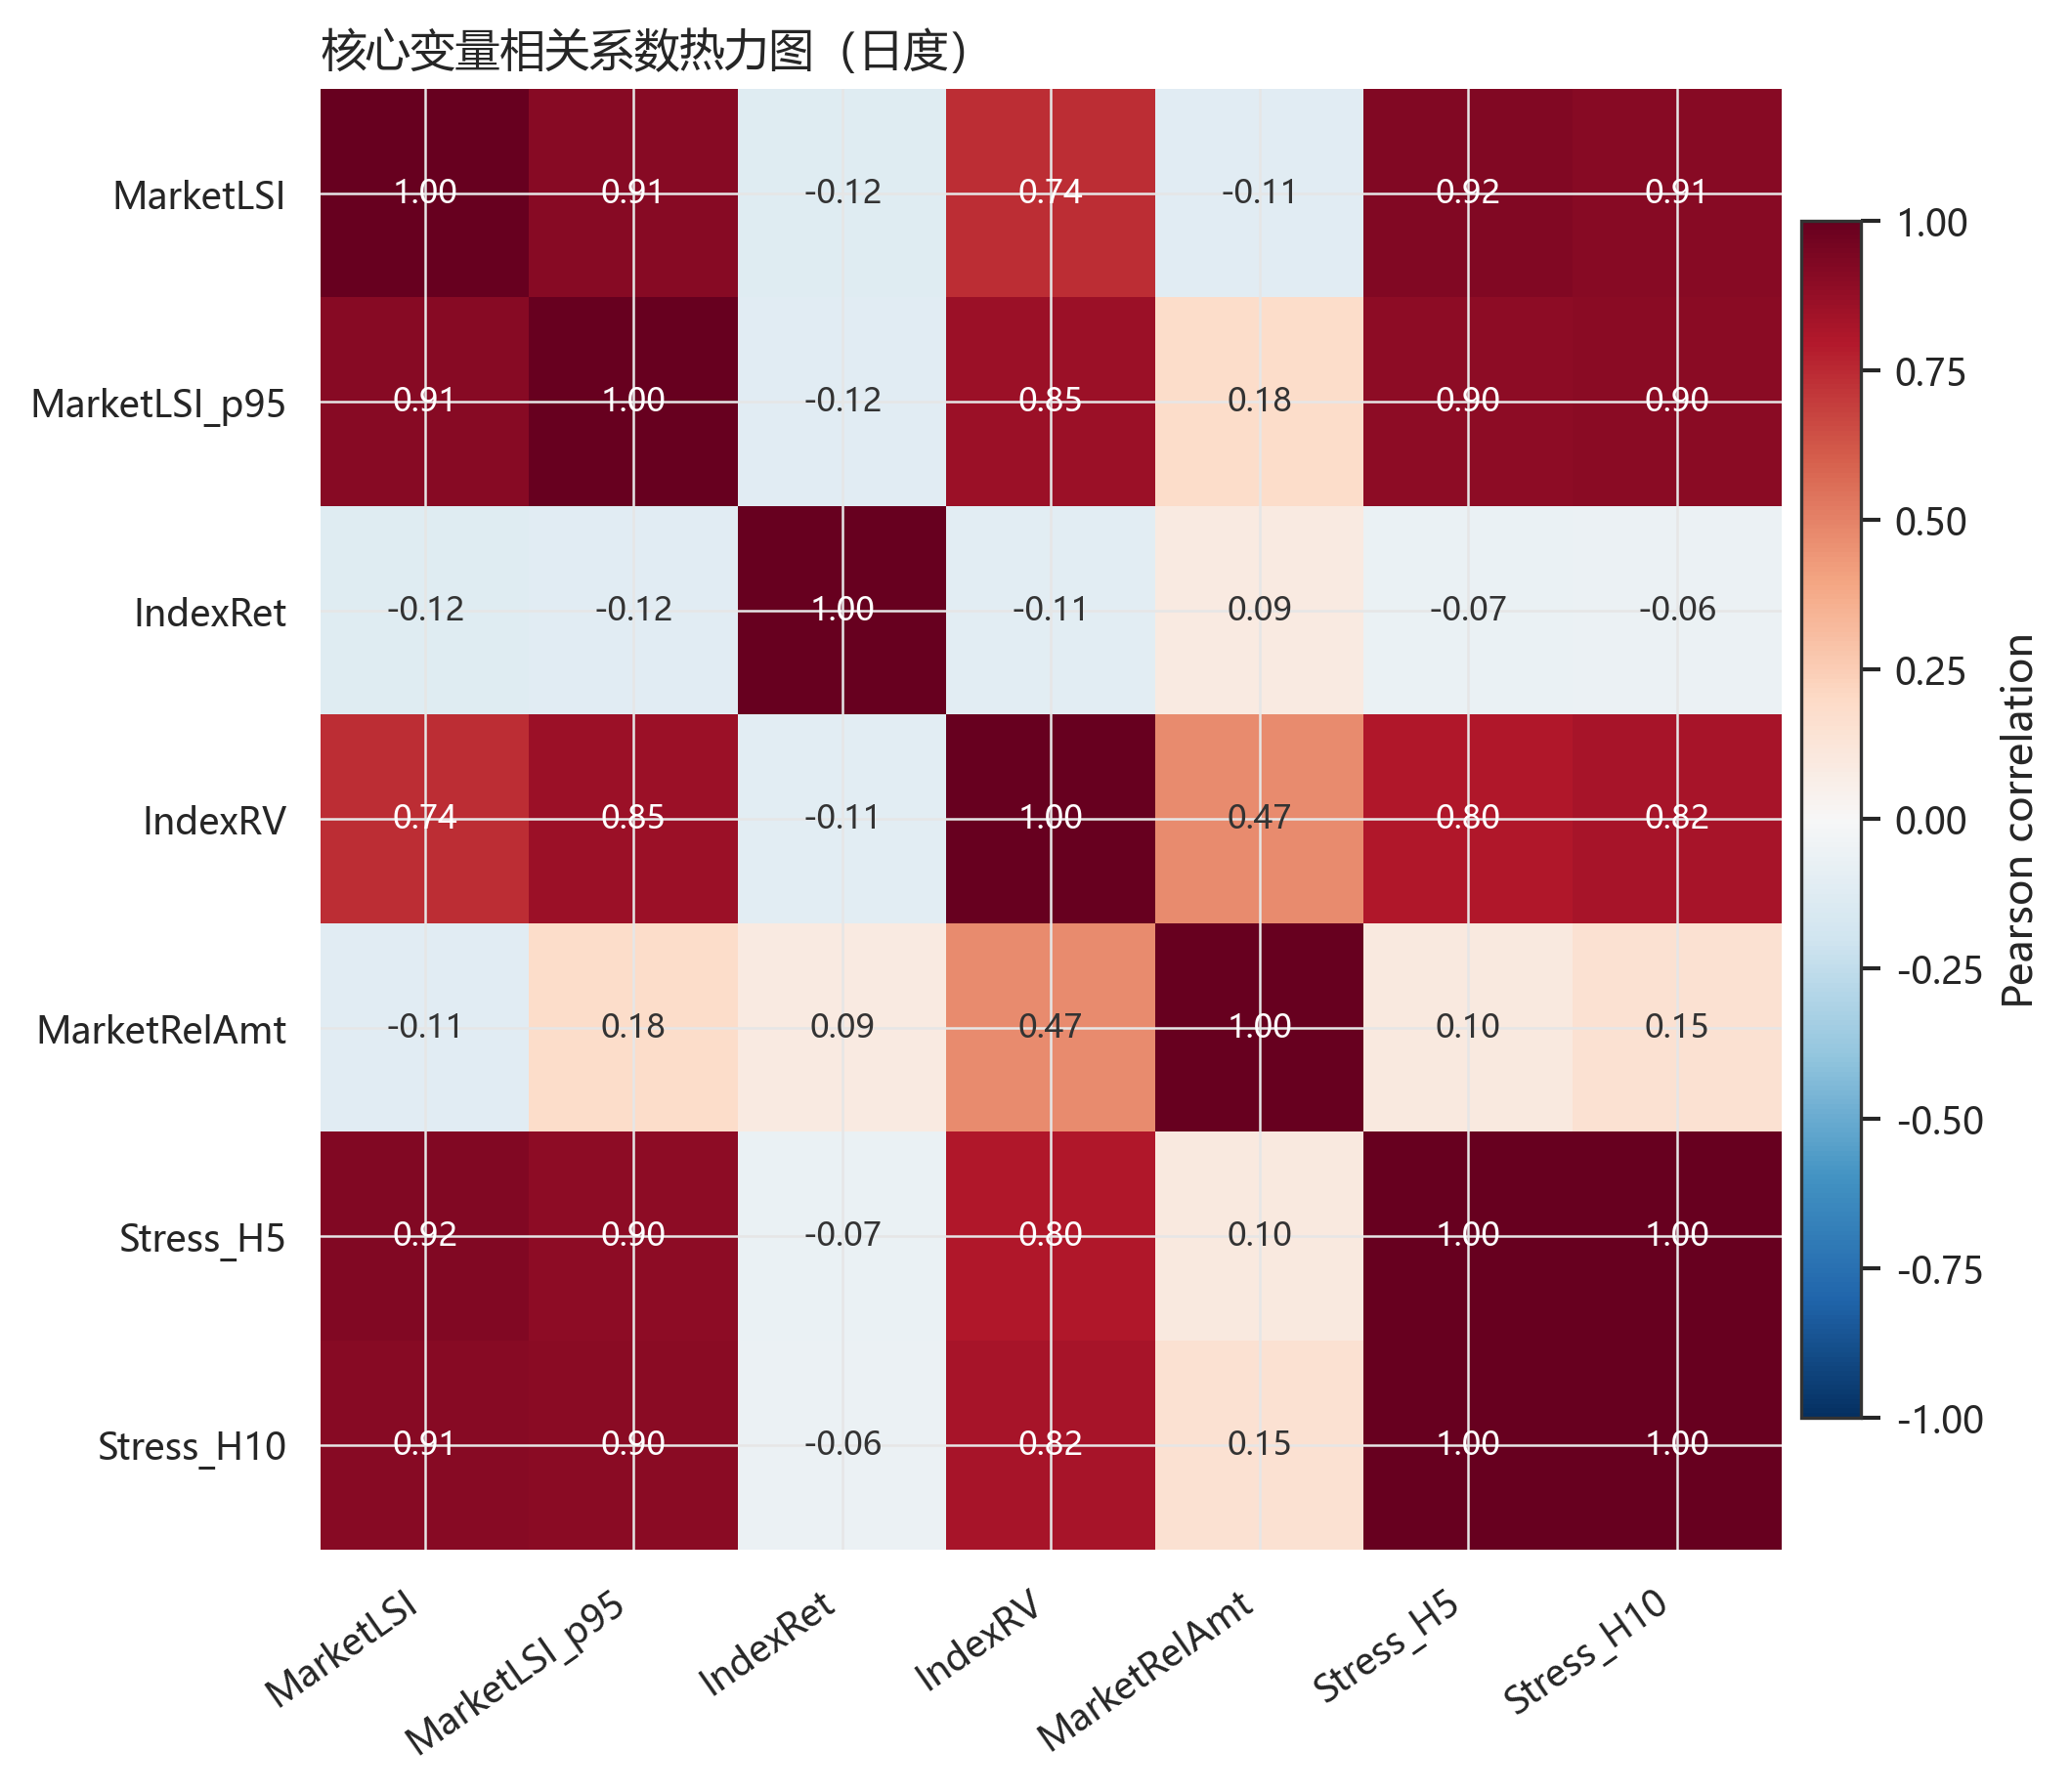
\includegraphics[width=0.76\textwidth]{figures/fig_corr.png}
    \caption{核心市场状态变量相关性热力图（日度）}
    \label{fig:app-corr}
\end{figure}


\subsection{模型诊断补充图}

图 \ref{fig:app-sb-calibration} 展示 SMARTBoost 概率输出的样本外校准曲线。校准曲线接近 45° 对角线说明预测概率具有一定的绝对校准精度；本文的核心关切集中于高风险排序能力，概率校准作为辅助证据。

\begin{figure}[!htbp]
    \centering
    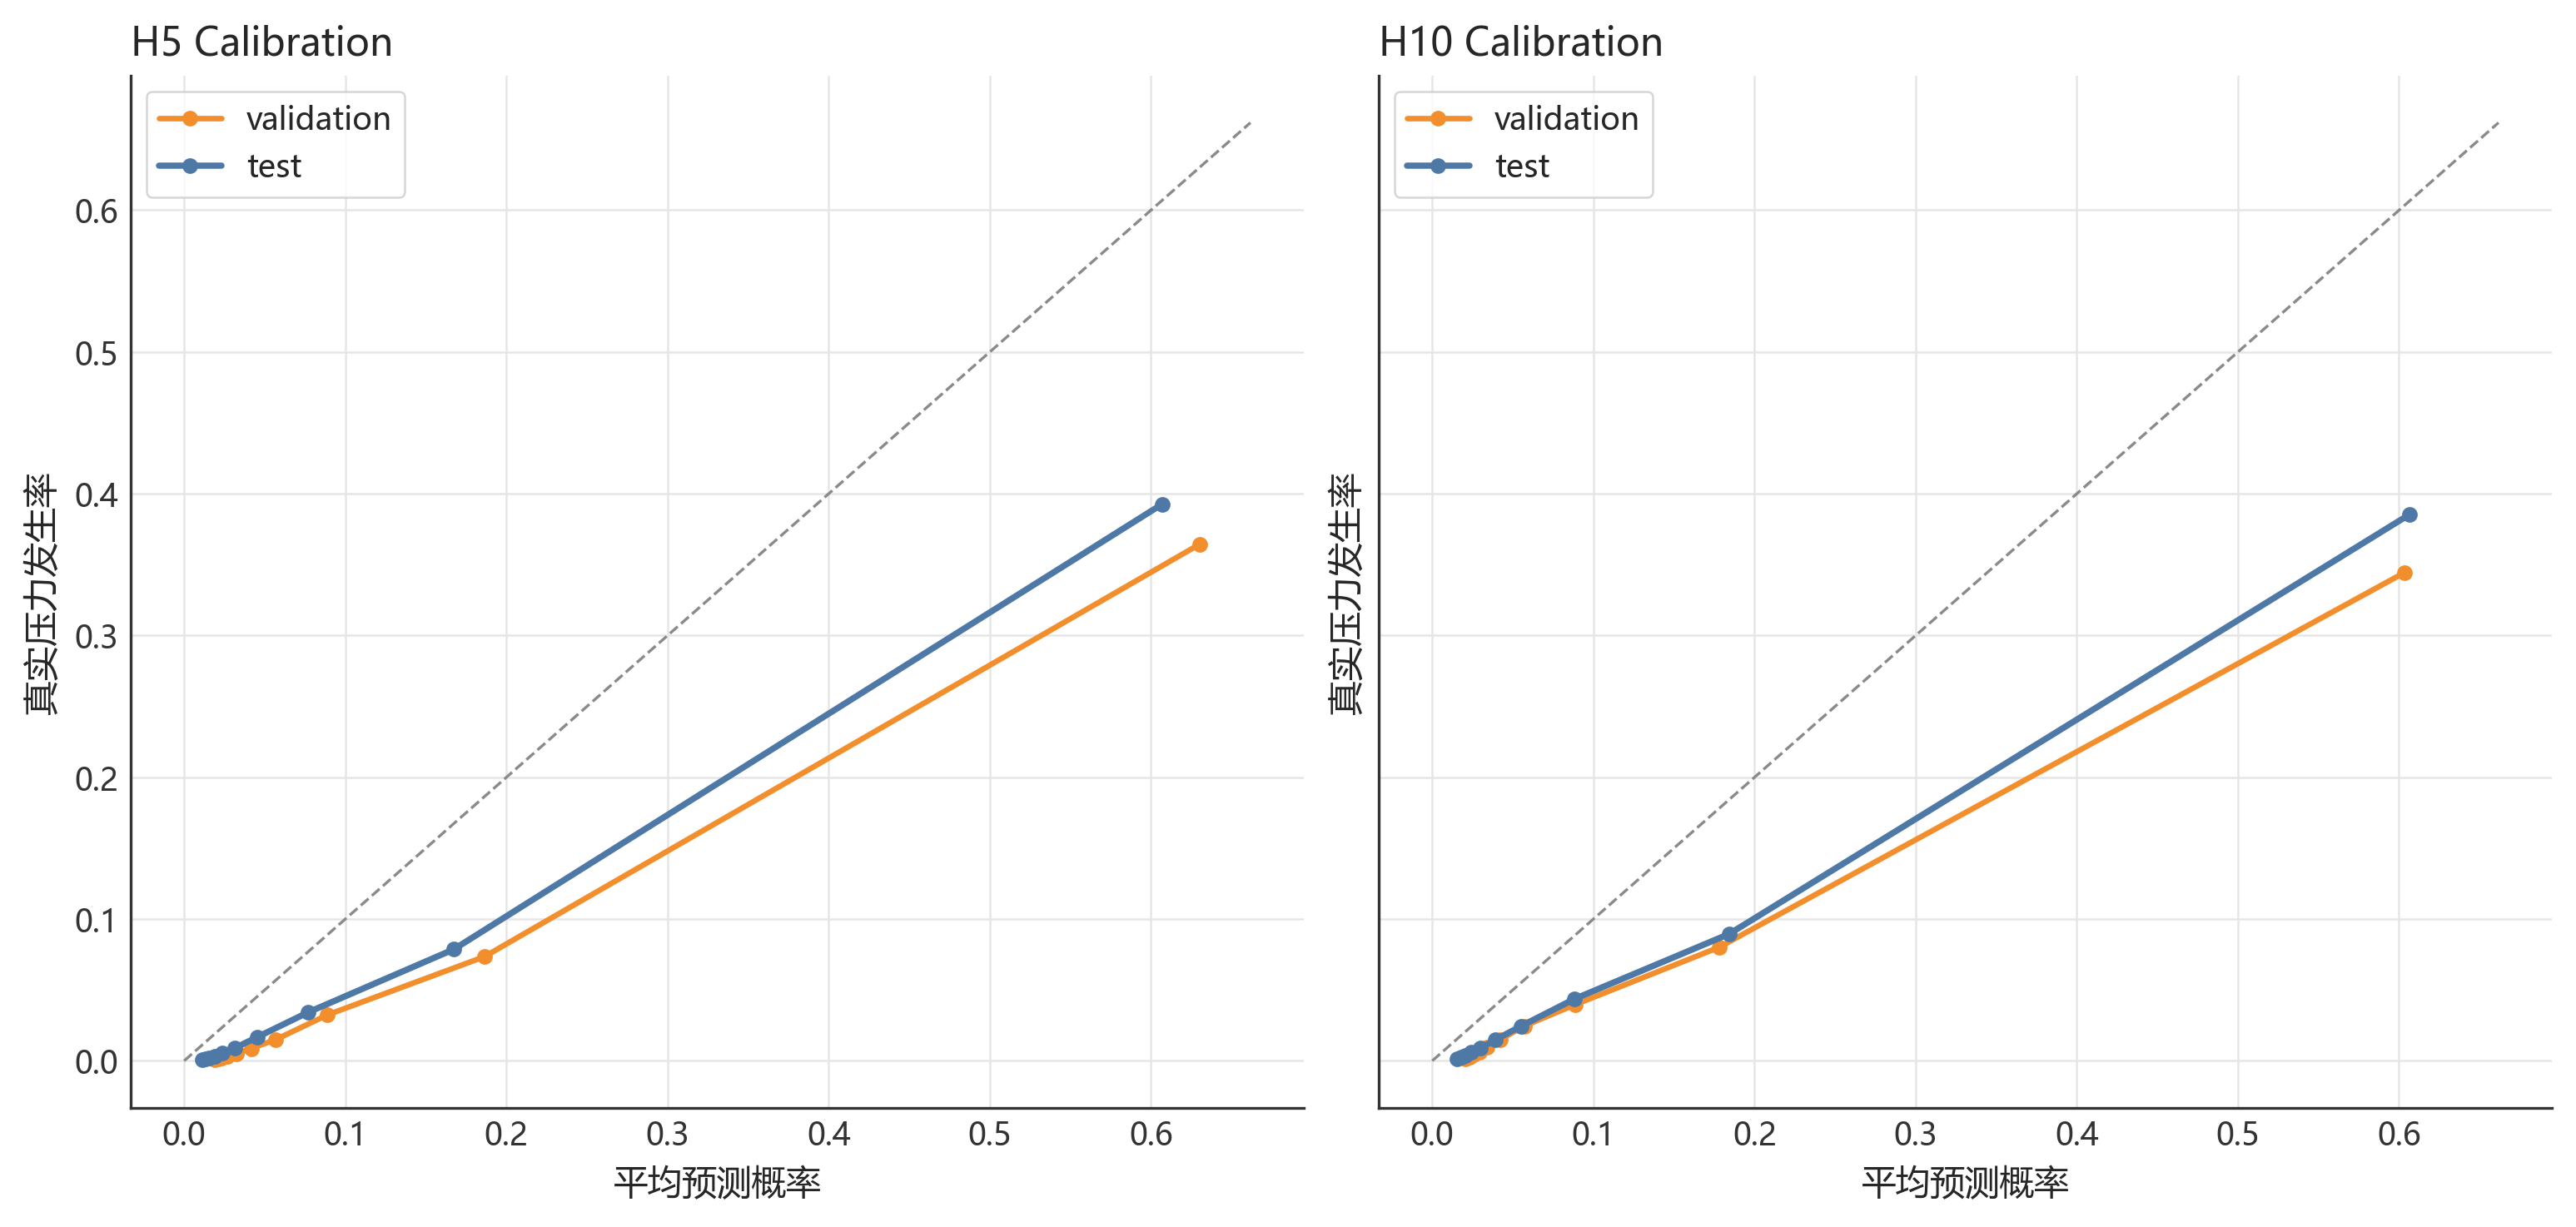
\includegraphics[width=0.86\textwidth]{figures/fig_sb_calibration.png}
    \caption{SMARTBoost 样本外校准曲线}
    \label{fig:app-sb-calibration}
\end{figure}

\FloatBarrier
\clearpage

\bibliographystyle{plain}
\bibliography{refs}

\end{document}
